%styles
%Da Latex für englischsprachige Texte ausgerichtet ist,
%wird als Dokumentenklasse das "`scrbook"' von Markus Kohm verwendet.
%Dieses ist für deutschsprachige Texte ausgelegt.
%BCOR12mm: 12mm Bindekorrektur (Verbreiterung des linken Randes)
%DIV11: entspricht in etwas der geforderten Textgröße und Seitenränder
%titlepage: eine Titelseite wird verwendet
%a4paper: DIN A4
%oneside: für eine spätere einseitige Bedruckung
\documentclass[BCOR12mm,DIV11,titlepage,a4paper,oneside,10pt]{scrbook}


% Farben definieren
\usepackage{color}
\usepackage[html]{xcolor}
\definecolor{m_green}{HTML}{00AD2F}
%\definecolor{m_pink}{HTML}{D40B6F}
\definecolor{m_pink}{HTML}{dd1166}
\definecolor{m_grey}{HTML}{555555}
\definecolor{m_lila}{HTML}{9313ce}
\definecolor{m_blau}{HTML}{4952e1}

% Paket Positionierung von Grafiken
\usepackage[export]{adjustbox}

%Paket für deutsche Silbentrennung etc.
\usepackage{ngerman}

%Paket für Zeichenkodierung, entspricht UTF-8
\usepackage[utf8x]{inputenc}

\usepackage{tocloft}
\newcommand{\listfootnotesname}{Fußnoten}% 'Fußnoten' title
\newlistof{footnotes}{fnt}{\listfootnotesname}% New 'List of...' for footnotes
\let\oldfootnote\footnote % Save the old \footnote{...} command
\renewcommand\footnote[1]{% Redefine the new footnote to also add 'List of Footnote' entries.
    \refstepcounter{footnotes}% Add and step a reference to the footnote/counter.
    \oldfootnote{#1}% Make a regular footnote.
    \addcontentsline{fnt}{footnotes}{\protect\numberline{\thefootnotes}#1}% Add the 'List of...' entry.
}

\newcommand{\listattachmentsname}{Anhang}% 'Anhang' title
\newlistof{attachments}{att}{\listattachmentsname}% New 'List of...' for attachments

%Paket das die Ausgabefonts definiert
\usepackage[T1]{fontenc}

%Paket für das Einbinden von Grafiken über die figure-Umgebung
\usepackage{graphicx}
\usepackage{grffile}

\usepackage{float}

\usepackage{mdframed}
\newmdenv[
  topline=false,
  bottomline=false,
  rightline=false,
  linewidth=2pt,
  linecolor=m_pink,
  innertopmargin=14pt,
  innerbottommargin=14pt,
  backgroundcolor=black!5,
  skipabove=\topsep,
  skipbelow=\topsep
]{siderules}

%Paket für mehrseitige Tabellen
\usepackage{longtable}
\setlength\LTleft{0pt}
\setlength\LTright{0pt}

\usepackage{booktabs}

%Paket zum \UTF{0192}ndern der Kopf- und Fußzeile
\usepackage{fancyhdr}

%Benutzt das Paket für eigenen Seitenstil
\pagestyle{fancy}

%Erzeugt eine Linie in der Kopfzeile (lässt sich mit 0.0pt ausblenden)
\renewcommand*{\headrulewidth}{0.1pt}
\renewcommand{\headrule}{\hbox to\headwidth{%
  \color{m_pink}\leaders\hrule height \headrulewidth\hfill}}
\lhead{} %Kopfzeile links

%\chead{\thepage} %Kopfzeile mitte
\chead{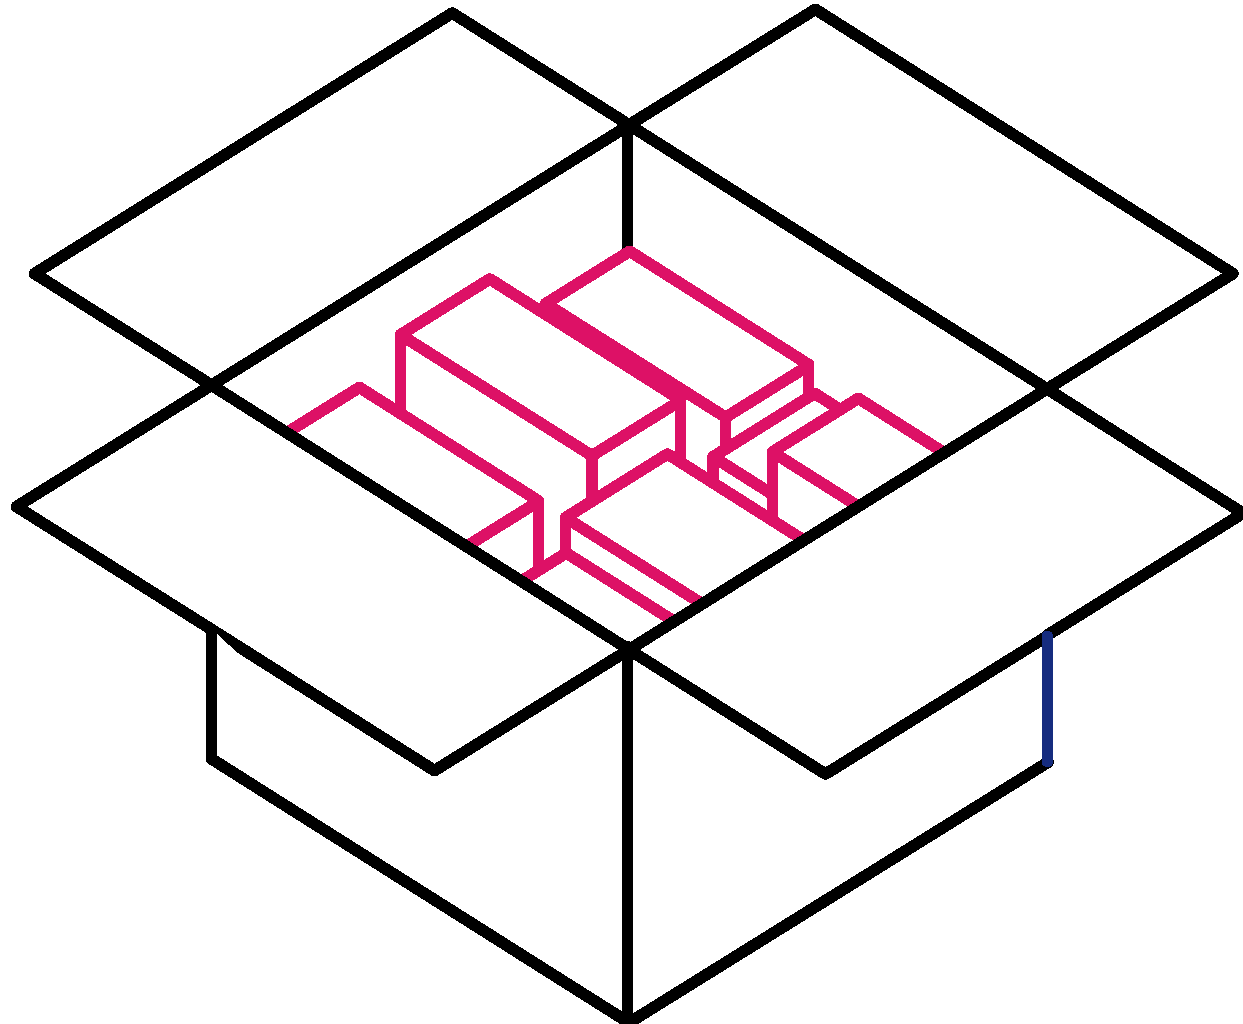
\includegraphics[height=20pt]{../assets/box.pdf}}
\rhead{} %Kopfzeile rechts
\lfoot{} %Fußzeile links
\cfoot{} %Fußzeile mitte
\rfoot{} %Fußzeile rechts
\makeatother


\newcommand{\changefont}{%
    \fontsize{9}{11}\selectfont
}


\setlength\headheight{60pt}
\setlength\footheight{40pt}
%\lfoot{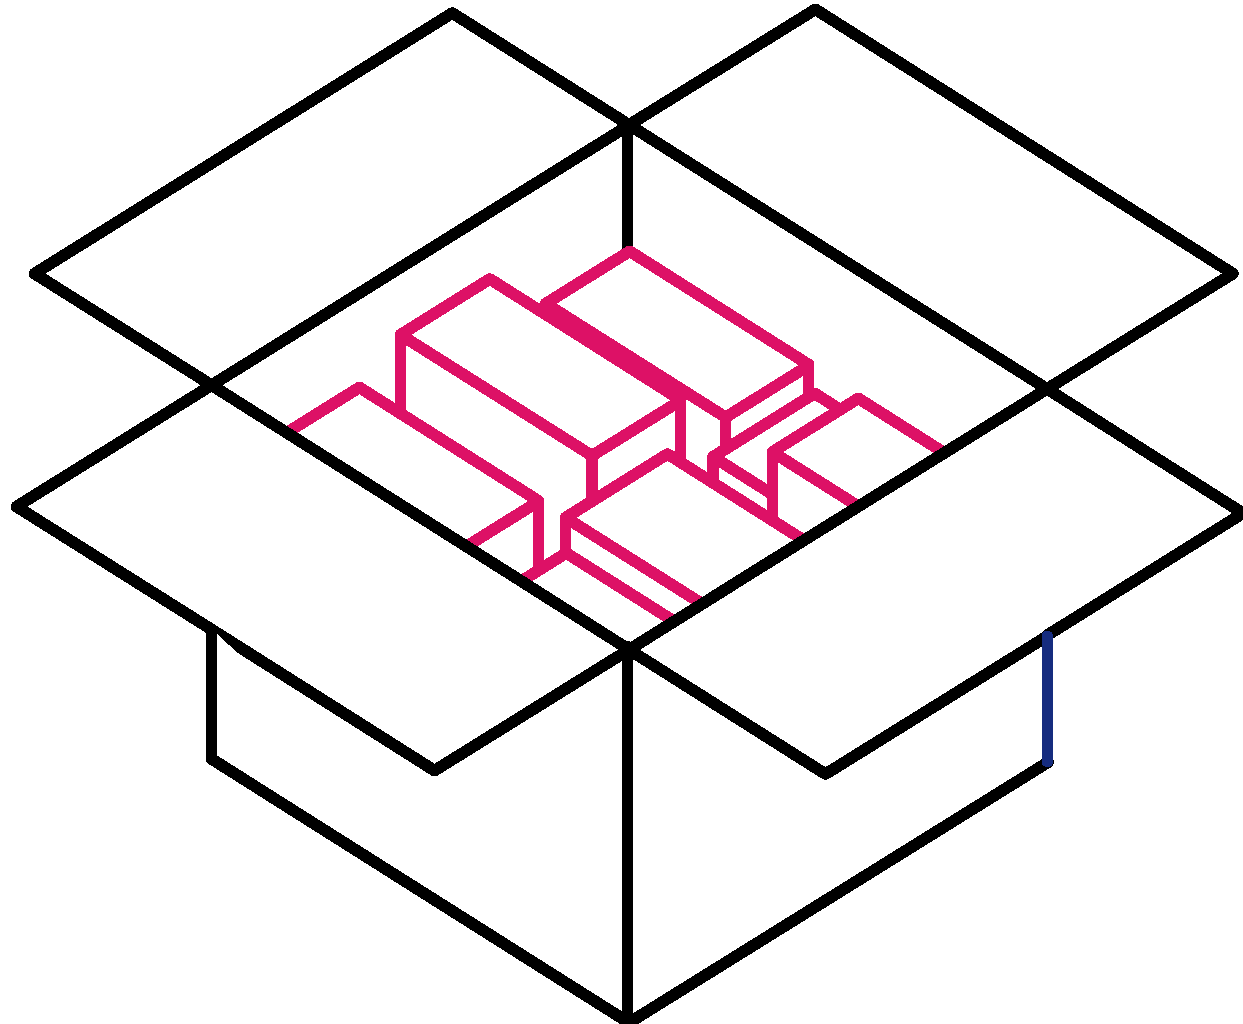
\includegraphics[height=40pt]{../assets/box.pdf}}
\rfoot{\thepage}
\lfoot{\changefont Selbstbericht Medieninformatik\\TH Köln // Institut für Informatik\\ \today}


%\UTF{0192}ndert die Seitennummerierung beim Inhaltsverzeichnis mit eigenem Stil
\renewcommand*{\indexpagestyle}{fancy}
%Verhindert die Seitennummerierung auf den Part-Seiten
\renewcommand*{\partpagestyle}{empty}
%\UTF{0192}ndert die Seitennummerierung bei Chapter mit eigenem Stil
\renewcommand*{\chapterpagestyle}{fancy}

%Abbildungsnummerierung ändern (abhängig von chapter, z.B. Abbildung 1.1)
\renewcommand*{\thefigure}{\thechapter.\arabic{figure}}
%Tabellennummerierung ändern (abhängig von chapter, z.B. Tabelle 1.1)
\renewcommand*{\thetable}{\thechapter.\arabic{table}}

%Paket, um ein Glossar/Abkürzungsverzeichnis anzulegen
\usepackage{nomencl}
\let\abbrev\nomenclature
%Der Name wird in Glossar geändert
\renewcommand{\nomname}{Glossar}
%Definiert die Aufteilung im Glossar zwischen Begriffen und Erläuterung
\setlength{\nomlabelwidth}{.25\hsize}
%Definiert die Punktelinien im Glossar
\renewcommand{\nomlabel}[1]{#1 \dotfill}
\setlength{\nomitemsep}{-\parsep}
%Veranlasst die Erstellung des Glossars
\makenomenclature

%Einrückungen nach Absätzen und Grafiken verhindern
\setlength{\parindent}{0pt}

%Verhindern, dass eine neue Seite für ein einzelnes Wort/Zeile verwendet wird
\clubpenalty = 10000 % schliesst Schusterjungen aus
\widowpenalty = 10000 % schliesst Hurenkinder aus (keine Beleidigung, sondern wirklich ein Fachbegriff)

%Paket für ein deutsches Literaturverzeichnis
\usepackage{bibgerm}

%Paket für die Verwendung von URLs durch den Befehl \url{}
%\usepackage{url}
\usepackage[hyphens]{url}

%Paket für Zeilenabstand (onehalfspace, singlespace)
\usepackage{setspace}

%Paket zur Erzeugung von Anführungszeichen durch \enquote{Text}
\usepackage[ngerman]{babel}
\usepackage[babel, german=quotes]{csquotes}

%Paket für farbigen Text
%black,white,green,red,blue,yellow,cyan,magenta
\usepackage{color}

%Paket für farbigen Hintergrund für Verbatim-Umgebung (Quelltext-Umgebung)
\usepackage{fancyvrb}
\usepackage{verbatim,moreverb}
%Grauton für Quelltext-Umgebung definieren 80% Grau
\definecolor{sourcegray}{gray}{.80}
%Paket für Quelltext-Umgebung
\usepackage{listings}

%Paket für Positionierung der Objekte ohne Float (Verwendungsbsp.: \begin{figure}[H])
\usepackage{float}

%Paket zur Erzeugung von Hyperrefs und PDF Informationen
\usepackage[pdftex,plainpages=false,pdfpagelabels,
            pdftitle={ Selbstbericht Medieninformatik // TH Köln // Institut für Informatik},
            pdfauthor={}
            ]{hyperref}
\hypersetup{
    colorlinks = true
}
\usepackage{pdfpages}

\providecommand{\tightlist}{%
  \setlength{\itemsep}{0pt}\setlength{\parskip}{0pt}}

\usepackage{tabularx}
\newcolumntype{L}[1]{>{\raggedright\arraybackslash}p{#1}}
\newcolumntype{C}[1]{>{\centering\arraybackslash}p{#1}}
\newcolumntype{R}[1]{>{\raggedleft\arraybackslash}p{#1}}

% URL
\PassOptionsToPackage{hyphens}{url}
\usepackage[pdftex]{hyperref}

% Sonderzeichen
\usepackage{textcomp}
\usepackage{eurosym}

\usepackage{setspace}
\renewcommand{\baselinestretch}{1.2}
\setlength{\parskip}{1em}

\usepackage[sfdefault,light]{roboto}  %% Option 'sfdefault' only if the base font of the document is to be sans serif


\usepackage[raggedright]{titlesec}
\titleformat{\chapter}[display]
  {\normalfont\sffamily\mdseries}
  {}{14pt}{\huge\raggedright}
% {\chaptertitlename\ \thechapter}{14pt}{\huge\raggedright}
\titleformat{\section}
  {\singlespacing\normalfont\sffamily\mdseries\Large\color{m_pink}\raggedright}
  {\thesection}{1em}{\Large}
\titleformat{\subsection}
  {\singlespacing\normalfont\sffamily\mdseries\large\raggedright}
  {\thesubsection}{1em}{\large}
% Zeilenumbruch und Spacing für Absätze
\titleformat{\paragraph}[hang]
  {\singlespacing\normalfont\normalsize\bfseries}
  {\theparagraph}{1em}{}
\titlespacing*{\paragraph}{0pt}{3.25ex plus 1ex minus .2ex}{0.5em}


\usepackage[font=footnotesize]{caption}


% Footer definieren
\makeatletter
\def\footrule{{
  \vskip-\footruleskip\vskip-\footrulewidth
  \color{\footrulecolor}
  \hrule\@width\headwidth\@height
  \footrulewidth\vskip\footruleskip
}}
\makeatother
\renewcommand{\footrulewidth}{0.1pt}
\newcommand{\footrulecolor}{m_green}



\begin{document}

%=== Deckblatt =======================================================
% Coversheet

\begin{titlepage}

	\includegraphics[width=0.25\textwidth]{../../../assets/logo_th_koeln.pdf}

	\vspace{2cm}
	{\Large\raggedright Erläuterung zur Erfüllung der im Akkreditierungsbericht formulierten Auflagen\par}
	\vspace{1cm}
	{\Large TH Köln – Campus Gummersbach \\ Fakultät für Informatik und Ingenieurwissenschaften \\ Institut für Informatik\par}

	\vfill

% Bottom of the page
	{\large \today\par}
\end{titlepage}


%=== Inhaltsverzeichnis ==============================================
\tableofcontents

%=== Hauptteil =======================================================
%Seitennummerierung des Hauptteils
\mainmatter


\hypertarget{advanced-seminar-projektpathlabel....srcmodulbeschreibungen-bachelor-bpo5ba_advanced-seminar}{%
\chapter{Advanced Seminar
(Projekt)\label{../../src/modulbeschreibungen-bachelor-bpo5/BA_Advanced-Seminar}}\label{advanced-seminar-projektpathlabel....srcmodulbeschreibungen-bachelor-bpo5ba_advanced-seminar}}

\begin{modulHead}
\textbf{Modulverantwortlich}: Prof.~Dr.~Mirjam
Blümm
\end{modulHead}
\begin{modulHead}
\textbf{Studiensemester}:
3
\end{modulHead}
\begin{modulHead}
\textbf{Sprache}:
deutsch
\end{modulHead}
\begin{modulHead}
\textbf{Kreditpunkte}:
5
\end{modulHead}
\begin{modulHead}
\textbf{Typ}:
Pflichtmodul
\end{modulHead}
\begin{modulHead}
\textbf{Prüfungsleistung}:
Projektarbeit, Fachvortrag mit Diskussion
\end{modulHead}


\hypertarget{sprachepathlabel....srcmodulbeschreibungen-bachelor-bpo5ba_advanced-seminar}{%
\section*{Sprache\label{../../src/modulbeschreibungen-bachelor-bpo5/BA_Advanced-Seminar}}\label{sprachepathlabel....srcmodulbeschreibungen-bachelor-bpo5ba_advanced-seminar}}

deutsch

\hypertarget{huxe4ufigkeit-des-angebotspathlabel....srcmodulbeschreibungen-bachelor-bpo5ba_advanced-seminar}{%
\section*{Häufigkeit des
Angebots\label{../../src/modulbeschreibungen-bachelor-bpo5/BA_Advanced-Seminar}}\label{huxe4ufigkeit-des-angebotspathlabel....srcmodulbeschreibungen-bachelor-bpo5ba_advanced-seminar}}

jedes Semester?

\hypertarget{dozierendepathlabel....srcmodulbeschreibungen-bachelor-bpo5ba_advanced-seminar}{%
\section*{Dozierende\label{../../src/modulbeschreibungen-bachelor-bpo5/BA_Advanced-Seminar}}\label{dozierendepathlabel....srcmodulbeschreibungen-bachelor-bpo5ba_advanced-seminar}}

Mirjam Blümm

\hypertarget{learning-outcomepathlabel....srcmodulbeschreibungen-bachelor-bpo5ba_advanced-seminar}{%
\section*{Learning
Outcome\label{../../src/modulbeschreibungen-bachelor-bpo5/BA_Advanced-Seminar}}\label{learning-outcomepathlabel....srcmodulbeschreibungen-bachelor-bpo5ba_advanced-seminar}}

WAS:

\begin{itemize}
\tightlist
\item
  ein Thema aus dem Projektfeld identifizieren, durch
  Literaturrecherchen erarbeiten und in Bezug zum Projekt und zu
  vergleichbaren Ansätzen bringen
\item
  wissenschaftliche Zusammenarbeit einüben (Peer Review)
\item
  Ergebnisse in einer Gruppen- oder Einzelarbeit (= Posterabstract \&
  Poster), die den Gepflogenheiten wissenschaftlicher Publikationen
  genügt, mit eigenen Worten darstellen und den anderen
  Seminarteilnehmenden präsentieren.
\end{itemize}

WOMIT

\begin{itemize}
\tightlist
\item
  Informationsmittel der Informatik; Recherche in Fachportalen \&
  -Datenbanken
\item
  mehrere Forschungsansätze detailliert verfolgen und nachvollziehen
  (statt eines generellen Überblicks über ein Thema) anhand
  peer-reviewter Paper, Studien, Experimente\ldots{}
\item
  Feedback-Prozess unter den Teilnehmenden (Peer Review)
\end{itemize}

WOZU

Wissenschaftliche Diskurse

\begin{itemize}
\tightlist
\item
  verstehen,
\item
  reflektieren \&
\item
  adäquat, ihn ihrer Fachlichkeit wiedergeben können
\end{itemize}

Grundvoraussetzung für wissenschaftliches Arbeiten (z.B. Bachelor
Thesis)

\hypertarget{modulinhaltepathlabel....srcmodulbeschreibungen-bachelor-bpo5ba_advanced-seminar}{%
\section*{Modulinhalte\label{../../src/modulbeschreibungen-bachelor-bpo5/BA_Advanced-Seminar}}\label{modulinhaltepathlabel....srcmodulbeschreibungen-bachelor-bpo5ba_advanced-seminar}}

\begin{itemize}
\tightlist
\item
  Lieraturrecherche, Recherchestrategien \& Suchfunktionen
\item
  (wissenschatliche) Quellen beurteiln
\item
  Zitieren und Zitierstile
\item
  Peer Review
\item
  Wissenschaftliches Schreiben \& Schreibstrategien
\end{itemize}

\hypertarget{lehr--und-lernmethodenpathlabel....srcmodulbeschreibungen-bachelor-bpo5ba_advanced-seminar}{%
\section*{Lehr- und
Lernmethoden\label{../../src/modulbeschreibungen-bachelor-bpo5/BA_Advanced-Seminar}}\label{lehr--und-lernmethodenpathlabel....srcmodulbeschreibungen-bachelor-bpo5ba_advanced-seminar}}

\begin{itemize}
\tightlist
\item
  flippeed classroom
\item
  Foliengestützte Vorlesung
\item
  Diskussionsrunden
\end{itemize}

\hypertarget{empfohlene-literaturpathlabel....srcmodulbeschreibungen-bachelor-bpo5ba_advanced-seminar}{%
\section*{Empfohlene
Literatur\label{../../src/modulbeschreibungen-bachelor-bpo5/BA_Advanced-Seminar}}\label{empfohlene-literaturpathlabel....srcmodulbeschreibungen-bachelor-bpo5ba_advanced-seminar}}

Esselborn-Krumbiegel, Helga. 2021. Von der Idee zum Text: eine Anleitung
zum wissenschaftlichen Schreiben. 6., aktualisierte Auflage. Paderborn:
Brill Schöningh.

\hypertarget{algorithmen-und-programmierung-1pathlabel....srcmodulbeschreibungen-bachelor-bpo5ba_algorithmenundprogrammierung1}{%
\chapter{Algorithmen und Programmierung
1\label{../../src/modulbeschreibungen-bachelor-bpo5/BA_AlgorithmenundProgrammierung1}}\label{algorithmen-und-programmierung-1pathlabel....srcmodulbeschreibungen-bachelor-bpo5ba_algorithmenundprogrammierung1}}

\begin{modulHead}
\textbf{Modulverantwortlich}: Prof.~Dr.~Frank
Victor
\end{modulHead}
\begin{modulHead}
\textbf{Studiensemester}:
1
\end{modulHead}
\begin{modulHead}
\textbf{Sprache}:
deutsch
\end{modulHead}
\begin{modulHead}
\textbf{Kreditpunkte}:
8
\end{modulHead}
\begin{modulHead}
\textbf{Typ}:
Pflichtmodul
\end{modulHead}
\begin{modulHead}
\textbf{Prüfungsleistung}:
Schriftliche Prüfung, sowie erfolgreiche Teilnahme am Praktikum als
Prüfungsvorleistung
\end{modulHead}


\hypertarget{lehrformswspathlabel....srcmodulbeschreibungen-bachelor-bpo5ba_algorithmenundprogrammierung1}{%
\section*{Lehrform/SWS\label{../../src/modulbeschreibungen-bachelor-bpo5/BA_AlgorithmenundProgrammierung1}}\label{lehrformswspathlabel....srcmodulbeschreibungen-bachelor-bpo5ba_algorithmenundprogrammierung1}}

6 SWS: Vorlesung 3 SWS; Übung 1 SWS; Praktikum 2 SWS

\hypertarget{arbeitsaufwandpathlabel....srcmodulbeschreibungen-bachelor-bpo5ba_algorithmenundprogrammierung1}{%
\section*{Arbeitsaufwand\label{../../src/modulbeschreibungen-bachelor-bpo5/BA_AlgorithmenundProgrammierung1}}\label{arbeitsaufwandpathlabel....srcmodulbeschreibungen-bachelor-bpo5ba_algorithmenundprogrammierung1}}

Gesamtaufwand 240h, davon

\begin{itemize}
\tightlist
\item
  54h Vorlesung
\item
  36h Praktikum
\item
  18h Übung
\item
  132h Selbststudium
\end{itemize}

\hypertarget{angestrebte-lernergebnissepathlabel....srcmodulbeschreibungen-bachelor-bpo5ba_algorithmenundprogrammierung1}{%
\section*{Angestrebte
Lernergebnisse\label{../../src/modulbeschreibungen-bachelor-bpo5/BA_AlgorithmenundProgrammierung1}}\label{angestrebte-lernergebnissepathlabel....srcmodulbeschreibungen-bachelor-bpo5ba_algorithmenundprogrammierung1}}

Die Studierenden sollen

\begin{itemize}
\tightlist
\item
  formale und algorithmische Kompetenzen im Bereich der
  Software-Entwicklung erlangen. Hierzu gehören insbesondere die
  Prinzipien der Objektorientierung und die der prozeduralen
  Programmierung.
\item
  die Kompetenz erlangen, strukturierte und unstrukturierte
  Problemstellungen zu analysieren, Lösungen modellbasiert zu entwickeln
  sowie prozedural und objektorientiert umzusetzen.
\item
  Systementwürfe evaluieren und bewerten können, insbesondere sollen sie
  die Arbeitsweise, die Randbedingungen und den Komplexitätsgrad von
  einfachen Algorithmen verstehen.
\item
  die Fähigkeit erlernen, algorithmische Entwurfsmuster zu erkennen und
  anzuwenden
\end{itemize}

\hypertarget{inhaltpathlabel....srcmodulbeschreibungen-bachelor-bpo5ba_algorithmenundprogrammierung1}{%
\section*{Inhalt\label{../../src/modulbeschreibungen-bachelor-bpo5/BA_AlgorithmenundProgrammierung1}}\label{inhaltpathlabel....srcmodulbeschreibungen-bachelor-bpo5ba_algorithmenundprogrammierung1}}

\begin{itemize}
\tightlist
\item
  Prozedurale Programmierung am Beispiel von C.
\item
  Objektorientierte Programmierung am Beispiel von Java.
\item
  Kontroll- und Datenstrukturen.
\item
  Modularisierungskonzepte.
\item
  Typkonzepte.
\item
  Grundmuster der objektorientierten Programmierung.
\item
  Elementare Algorithmen und Aufwandsschätzung.
\item
  Entwicklungsumgebungen.
\end{itemize}

\hypertarget{medienformenpathlabel....srcmodulbeschreibungen-bachelor-bpo5ba_algorithmenundprogrammierung1}{%
\section*{Medienformen\label{../../src/modulbeschreibungen-bachelor-bpo5/BA_AlgorithmenundProgrammierung1}}\label{medienformenpathlabel....srcmodulbeschreibungen-bachelor-bpo5ba_algorithmenundprogrammierung1}}

\begin{itemize}
\tightlist
\item
  Beamer-gestützte Vorlesungen (Folien in elektronischer Form)
\item
  Praktikum an Rechnern des Labors
\end{itemize}

\hypertarget{literaturpathlabel....srcmodulbeschreibungen-bachelor-bpo5ba_algorithmenundprogrammierung1}{%
\section*{Literatur\label{../../src/modulbeschreibungen-bachelor-bpo5/BA_AlgorithmenundProgrammierung1}}\label{literaturpathlabel....srcmodulbeschreibungen-bachelor-bpo5ba_algorithmenundprogrammierung1}}

\begin{itemize}
\tightlist
\item
  Vorlesungsunterlagen: Foliensammlung, ausformuliertes Skript,
  Beispiellösungen, Übungsklausuren mit Lösungen
\item
  Fachliteratur: Diverse C-Bücher, u.a.: Kernighan, B.W., Ritchie, D.M.:
  „Programmieren in C``
\item
  Diverse Java-Bücher, u.a.: Bishop, J.: „Java Lernen``
\item
  Sedgewick, R.: „Algorithmen in Java``
\end{itemize}

\hypertarget{algorithmen-und-programmierung-2pathlabel....srcmodulbeschreibungen-bachelor-bpo5ba_algorithmenundprogrammierung2}{%
\chapter{Algorithmen und Programmierung
2\label{../../src/modulbeschreibungen-bachelor-bpo5/BA_AlgorithmenundProgrammierung2}}\label{algorithmen-und-programmierung-2pathlabel....srcmodulbeschreibungen-bachelor-bpo5ba_algorithmenundprogrammierung2}}

\begin{modulHead}
\textbf{Modulverantwortlich}: Prof.~Dr.~Christian
Kohls
\end{modulHead}
\begin{modulHead}
\textbf{Studiensemester}:
2
\end{modulHead}
\begin{modulHead}
\textbf{Sprache}:
deutsch
\end{modulHead}
\begin{modulHead}
\textbf{Kreditpunkte}:
7
\end{modulHead}
\begin{modulHead}
\textbf{Typ}:
Pflichtmodul
\end{modulHead}
\begin{modulHead}
\textbf{Prüfungsleistung}:
Schriftliche Prüfung, sowie erfolgreiche Teilnahme am Praktikum als
Prüfungsvorleistung
\end{modulHead}


\hypertarget{besonderheitenpathlabel....srcmodulbeschreibungen-bachelor-bpo5ba_algorithmenundprogrammierung2}{%
\section*{Besonderheiten\label{../../src/modulbeschreibungen-bachelor-bpo5/BA_AlgorithmenundProgrammierung2}}\label{besonderheitenpathlabel....srcmodulbeschreibungen-bachelor-bpo5ba_algorithmenundprogrammierung2}}

\begin{center}\rule{0.5\linewidth}{0.5pt}\end{center}

\hypertarget{lehrformswspathlabel....srcmodulbeschreibungen-bachelor-bpo5ba_algorithmenundprogrammierung2}{%
\section*{Lehrform/SWS\label{../../src/modulbeschreibungen-bachelor-bpo5/BA_AlgorithmenundProgrammierung2}}\label{lehrformswspathlabel....srcmodulbeschreibungen-bachelor-bpo5ba_algorithmenundprogrammierung2}}

6 SWS: Vorlesung 3 SWS; Übung 1 SWS; Praktikum 2 SWS

\hypertarget{arbeitsaufwandpathlabel....srcmodulbeschreibungen-bachelor-bpo5ba_algorithmenundprogrammierung2}{%
\section*{Arbeitsaufwand\label{../../src/modulbeschreibungen-bachelor-bpo5/BA_AlgorithmenundProgrammierung2}}\label{arbeitsaufwandpathlabel....srcmodulbeschreibungen-bachelor-bpo5ba_algorithmenundprogrammierung2}}

Gesamtaufwand 210h, davon

\begin{itemize}
\tightlist
\item
  54h Vorlesung
\item
  36h Praktikum
\item
  18h Übung
\item
  102h Selbststudium
\end{itemize}

\hypertarget{angestrebte-lernergebnissepathlabel....srcmodulbeschreibungen-bachelor-bpo5ba_algorithmenundprogrammierung2}{%
\section*{Angestrebte
Lernergebnisse\label{../../src/modulbeschreibungen-bachelor-bpo5/BA_AlgorithmenundProgrammierung2}}\label{angestrebte-lernergebnissepathlabel....srcmodulbeschreibungen-bachelor-bpo5ba_algorithmenundprogrammierung2}}

Die Studierende sollen Objektorientierung, die Prinzipien der
Algorithmenentwicklung und grundlegende Algorithmen verstehen und die
Grundstrukturen der Java-Bibliothek anwenden können.

\hypertarget{inhaltpathlabel....srcmodulbeschreibungen-bachelor-bpo5ba_algorithmenundprogrammierung2}{%
\section*{Inhalt\label{../../src/modulbeschreibungen-bachelor-bpo5/BA_AlgorithmenundProgrammierung2}}\label{inhaltpathlabel....srcmodulbeschreibungen-bachelor-bpo5ba_algorithmenundprogrammierung2}}

\begin{itemize}
\tightlist
\item
  Basisalgorithmen: Suchen u. Sortieren
\item
  Datenstrukturen
\item
  Dictionaries
\item
  Methodik des objektorientierten Programmierens
\end{itemize}

\hypertarget{medienformenpathlabel....srcmodulbeschreibungen-bachelor-bpo5ba_algorithmenundprogrammierung2}{%
\section*{Medienformen\label{../../src/modulbeschreibungen-bachelor-bpo5/BA_AlgorithmenundProgrammierung2}}\label{medienformenpathlabel....srcmodulbeschreibungen-bachelor-bpo5ba_algorithmenundprogrammierung2}}

\begin{itemize}
\tightlist
\item
  Beamer-gestützte Vorlesungen (Folien in elektronischer Form)
\item
  Praktikum an Rechnern des Labors
\end{itemize}

\hypertarget{literaturpathlabel....srcmodulbeschreibungen-bachelor-bpo5ba_algorithmenundprogrammierung2}{%
\section*{Literatur\label{../../src/modulbeschreibungen-bachelor-bpo5/BA_AlgorithmenundProgrammierung2}}\label{literaturpathlabel....srcmodulbeschreibungen-bachelor-bpo5ba_algorithmenundprogrammierung2}}

\begin{itemize}
\tightlist
\item
  Vorlesungsunterlagen: Foliensammlung, ausformuliertes Skript,
  Beispiellösungen
\item
  Fachliteratur: Bishop, J.: „Java Lernen``
\item
  Sedgewick, R.: „Algorithmen in Java``
\item
  Barnes, J., Kölling, M.: „Java Lernen mit BlueJ``, Verweise auf
  Onlinedokumente
\end{itemize}

\hypertarget{bachelorarbeitpathlabel....srcmodulbeschreibungen-bachelor-bpo5ba_bachelorarbeit}{%
\chapter{Bachelorarbeit\label{../../src/modulbeschreibungen-bachelor-bpo5/BA_Bachelorarbeit}}\label{bachelorarbeitpathlabel....srcmodulbeschreibungen-bachelor-bpo5ba_bachelorarbeit}}

\begin{modulHead}
\textbf{Modulverantwortlich}: alle Professor:innen
der TH Köln
\end{modulHead}
\begin{modulHead}
\textbf{Studiensemester}:
7
\end{modulHead}
\begin{modulHead}
\textbf{Sprache}:
deutsch
\end{modulHead}
\begin{modulHead}
\textbf{Kreditpunkte}:
12
\end{modulHead}
\begin{modulHead}
\textbf{Typ}:
Pflichtmodul
\end{modulHead}
\begin{modulHead}
\textbf{Prüfungsleistung}:
Schriftliche Ausarbeitung, ggf. Projektarbeit mit entsprechenden
Artefakten.
\end{modulHead}


\hypertarget{besonderheitenpathlabel....srcmodulbeschreibungen-bachelor-bpo5ba_bachelorarbeit}{%
\section*{Besonderheiten\label{../../src/modulbeschreibungen-bachelor-bpo5/BA_Bachelorarbeit}}\label{besonderheitenpathlabel....srcmodulbeschreibungen-bachelor-bpo5ba_bachelorarbeit}}

\begin{center}\rule{0.5\linewidth}{0.5pt}\end{center}

\hypertarget{lehrformswspathlabel....srcmodulbeschreibungen-bachelor-bpo5ba_bachelorarbeit}{%
\section*{Lehrform/SWS\label{../../src/modulbeschreibungen-bachelor-bpo5/BA_Bachelorarbeit}}\label{lehrformswspathlabel....srcmodulbeschreibungen-bachelor-bpo5ba_bachelorarbeit}}

Angeleitetes, eigenverantwortliches Arbeiten

\hypertarget{arbeitsaufwandpathlabel....srcmodulbeschreibungen-bachelor-bpo5ba_bachelorarbeit}{%
\section*{Arbeitsaufwand\label{../../src/modulbeschreibungen-bachelor-bpo5/BA_Bachelorarbeit}}\label{arbeitsaufwandpathlabel....srcmodulbeschreibungen-bachelor-bpo5ba_bachelorarbeit}}

360 Stunden

\hypertarget{angestrebte-lernergebnissepathlabel....srcmodulbeschreibungen-bachelor-bpo5ba_bachelorarbeit}{%
\section*{Angestrebte
Lernergebnisse\label{../../src/modulbeschreibungen-bachelor-bpo5/BA_Bachelorarbeit}}\label{angestrebte-lernergebnissepathlabel....srcmodulbeschreibungen-bachelor-bpo5ba_bachelorarbeit}}

Die Bachelorarbeit soll zeigen, dass der Prüfling befähigt ist,
innerhalb einer vorgegebenen Frist eine praxisorientierte Aufgabe aus
seinem Fachgebiet sowohl in ihren fachlichen Einzelheiten als auch in
den fachübergreifenden Zusammenhängen nach wissenschaftlichen,
fachpraktischen und gestalterischen Methoden selbständig zu bearbeiten.
Die Bachelorarbeit ist in der Regel eine eigenständige Untersuchung mit
einer Aufgabenstellung aus der Medieninformatik und einer ausführlichen
Beschreibung und Erläuterung ihrer Lösung. In fachlich geeigneten Fällen
kann sie auch eine schriftliche Hausarbeit mit fachliterarischem Inhalt
sein.

\hypertarget{inhaltpathlabel....srcmodulbeschreibungen-bachelor-bpo5ba_bachelorarbeit}{%
\section*{Inhalt\label{../../src/modulbeschreibungen-bachelor-bpo5/BA_Bachelorarbeit}}\label{inhaltpathlabel....srcmodulbeschreibungen-bachelor-bpo5ba_bachelorarbeit}}

Selbstständiges wissenschaftliches, fachpraktisches und gestalterisches
Bearbeiten einer Aufgabenstellung.

\hypertarget{bachelor-kolloquiumpathlabel....srcmodulbeschreibungen-bachelor-bpo5ba_bachelorkolloquium}{%
\chapter{Bachelor
Kolloquium\label{../../src/modulbeschreibungen-bachelor-bpo5/BA_Bachelorkolloquium}}\label{bachelor-kolloquiumpathlabel....srcmodulbeschreibungen-bachelor-bpo5ba_bachelorkolloquium}}

\begin{modulHead}
\textbf{Modulverantwortlich}: alle Professor:innen
der TH Köln
\end{modulHead}
\begin{modulHead}
\textbf{Studiensemester}:
7
\end{modulHead}
\begin{modulHead}
\textbf{Sprache}:
deutsch
\end{modulHead}
\begin{modulHead}
\textbf{Kreditpunkte}:
3
\end{modulHead}
\begin{modulHead}
\textbf{Typ}:
Pflichtmodul
\end{modulHead}
\begin{modulHead}
\textbf{Prüfungsleistung}:
Mündliche Prüfung, Vortrag, Fachgespräch
\end{modulHead}


\hypertarget{besonderheitenpathlabel....srcmodulbeschreibungen-bachelor-bpo5ba_bachelorkolloquium}{%
\section*{Besonderheiten\label{../../src/modulbeschreibungen-bachelor-bpo5/BA_Bachelorkolloquium}}\label{besonderheitenpathlabel....srcmodulbeschreibungen-bachelor-bpo5ba_bachelorkolloquium}}

\begin{center}\rule{0.5\linewidth}{0.5pt}\end{center}

\hypertarget{lehrformswspathlabel....srcmodulbeschreibungen-bachelor-bpo5ba_bachelorkolloquium}{%
\section*{Lehrform/SWS\label{../../src/modulbeschreibungen-bachelor-bpo5/BA_Bachelorkolloquium}}\label{lehrformswspathlabel....srcmodulbeschreibungen-bachelor-bpo5ba_bachelorkolloquium}}

Angeleitetes, eigenverantwortliches Arbeiten

\hypertarget{arbeitsaufwandpathlabel....srcmodulbeschreibungen-bachelor-bpo5ba_bachelorkolloquium}{%
\section*{Arbeitsaufwand\label{../../src/modulbeschreibungen-bachelor-bpo5/BA_Bachelorkolloquium}}\label{arbeitsaufwandpathlabel....srcmodulbeschreibungen-bachelor-bpo5ba_bachelorkolloquium}}

90 Stunden

\hypertarget{angestrebte-lernergebnissepathlabel....srcmodulbeschreibungen-bachelor-bpo5ba_bachelorkolloquium}{%
\section*{Angestrebte
Lernergebnisse\label{../../src/modulbeschreibungen-bachelor-bpo5/BA_Bachelorkolloquium}}\label{angestrebte-lernergebnissepathlabel....srcmodulbeschreibungen-bachelor-bpo5ba_bachelorkolloquium}}

Das Kolloquium dient der Feststellung, ob der Prüfling befähigt ist, die
Ergebnisse der Bachelorarbeit, ihre fachlichen Grundlagen, ihre
fachübergreifenden Zusammenhänge und ihre außerfachlichen Bezüge
mündlich darzustellen und selbständig zu begründen und ihre Bedeutung
für die Praxis einzuschätzen. Dabei soll auch die Bearbeitung des Themas
der Bachelorarbeit mit dem Prüfling erörtert werden.

\hypertarget{inhaltpathlabel....srcmodulbeschreibungen-bachelor-bpo5ba_bachelorkolloquium}{%
\section*{Inhalt\label{../../src/modulbeschreibungen-bachelor-bpo5/BA_Bachelorkolloquium}}\label{inhaltpathlabel....srcmodulbeschreibungen-bachelor-bpo5ba_bachelorkolloquium}}

Vortrag über das Thema der Bachelorarbeit, Fachdiskussion und mündliche
Verteidigung der Arbeit im Kontext der Medieninformatik.

\hypertarget{communityprojektpathlabel....srcmodulbeschreibungen-bachelor-bpo5ba_communityprojekt}{%
\chapter{Communityprojekt\label{../../src/modulbeschreibungen-bachelor-bpo5/BA_Communityprojekt}}\label{communityprojektpathlabel....srcmodulbeschreibungen-bachelor-bpo5ba_communityprojekt}}

\begin{modulHead}
\textbf{Modulverantwortlich}: Prof.~Christian
Noss
\end{modulHead}
\begin{modulHead}
\textbf{Studiensemester}:
2
\end{modulHead}
\begin{modulHead}
\textbf{Sprache}:
deutsch
\end{modulHead}
\begin{modulHead}
\textbf{Kreditpunkte}:
5
\end{modulHead}
\begin{modulHead}
\textbf{Typ}:
Pflichtmodul
\end{modulHead}


\hypertarget{besonderheitenpathlabel....srcmodulbeschreibungen-bachelor-bpo5ba_communityprojekt}{%
\section*{Besonderheiten\label{../../src/modulbeschreibungen-bachelor-bpo5/BA_Communityprojekt}}\label{besonderheitenpathlabel....srcmodulbeschreibungen-bachelor-bpo5ba_communityprojekt}}

\begin{center}\rule{0.5\linewidth}{0.5pt}\end{center}

\hypertarget{datenbanksystemepathlabel....srcmodulbeschreibungen-bachelor-bpo5ba_datenbanksysteme}{%
\chapter{Datenbanksysteme\label{../../src/modulbeschreibungen-bachelor-bpo5/BA_Datenbanksysteme}}\label{datenbanksystemepathlabel....srcmodulbeschreibungen-bachelor-bpo5ba_datenbanksysteme}}

\begin{modulHead}
\textbf{Modulverantwortlich}: Prof.~Dr.~Johann
Schaible
\end{modulHead}
\begin{modulHead}
\textbf{Studiensemester}:
3
\end{modulHead}
\begin{modulHead}
\textbf{Sprache}:
deutsch
\end{modulHead}
\begin{modulHead}
\textbf{Kreditpunkte}:
5
\end{modulHead}
\begin{modulHead}
\textbf{Typ}:
Pflichtmodul
\end{modulHead}
\begin{modulHead}
\textbf{Prüfungsleistung}:
Schriftliche Prüfung, sowie erfolgreiche Teilnahme am Praktikum als
Prüfungsvorleistung.
\end{modulHead}


\hypertarget{sprachepathlabel....srcmodulbeschreibungen-bachelor-bpo5ba_datenbanksysteme}{%
\section*{Sprache\label{../../src/modulbeschreibungen-bachelor-bpo5/BA_Datenbanksysteme}}\label{sprachepathlabel....srcmodulbeschreibungen-bachelor-bpo5ba_datenbanksysteme}}

Deutsch

\hypertarget{huxe4ufigkeit-des-angebotspathlabel....srcmodulbeschreibungen-bachelor-bpo5ba_datenbanksysteme}{%
\section*{Häufigkeit des
Angebots\label{../../src/modulbeschreibungen-bachelor-bpo5/BA_Datenbanksysteme}}\label{huxe4ufigkeit-des-angebotspathlabel....srcmodulbeschreibungen-bachelor-bpo5ba_datenbanksysteme}}

Wintersemester

\hypertarget{dozierendepathlabel....srcmodulbeschreibungen-bachelor-bpo5ba_datenbanksysteme}{%
\section*{Dozierende\label{../../src/modulbeschreibungen-bachelor-bpo5/BA_Datenbanksysteme}}\label{dozierendepathlabel....srcmodulbeschreibungen-bachelor-bpo5ba_datenbanksysteme}}

Prof.~Dr.~Johann Schaible, Prof.~Dr.~Birgit Bertelsmeier

\hypertarget{learning-outcomepathlabel....srcmodulbeschreibungen-bachelor-bpo5ba_datenbanksysteme}{%
\section*{Learning
Outcome\label{../../src/modulbeschreibungen-bachelor-bpo5/BA_Datenbanksysteme}}\label{learning-outcomepathlabel....srcmodulbeschreibungen-bachelor-bpo5ba_datenbanksysteme}}

\begin{itemize}
\tightlist
\item
  Was: Sie sind in der Lage aus Anforderungskatalogen ein relationales
  Datenbankschema zu konzipieren, realisieren, und dieses abzufragen,
  indem Sie\ldots{}
\item
  Lehrinhalte:

  \begin{itemize}
\tightlist
\item
    Datenspezifikationen korrekt identifizieren und daraus ein
    konzeptionelles Modell erstellen,
  \item
    unter Beachtung von Normalisierungsregeln ein relationales Modell
    entwickeln,
  \item
    mit SQL ein Datenbankschema erzeugen und manipulieren,
  \item
    SQL SELECT-Statements für komplexe Datenabfragen anwenden, und
  \item
    effizienz-steigernde Methoden (SQL Tuning, Indexe) verwenden.
  \end{itemize}
\end{itemize}

\hypertarget{modulinhaltepathlabel....srcmodulbeschreibungen-bachelor-bpo5ba_datenbanksysteme}{%
\section*{Modulinhalte\label{../../src/modulbeschreibungen-bachelor-bpo5/BA_Datenbanksysteme}}\label{modulinhaltepathlabel....srcmodulbeschreibungen-bachelor-bpo5ba_datenbanksysteme}}

\begin{itemize}
\tightlist
\item
  Erstellung konzeptioneller Datenmodelle als Entity
  Relationship-Diagramm
\item
  Transformation des konzeptionellen Modells in das relationale Modell
  unter Beachtung der Normalformen
\item
  Physischer Entwurf einer Datenbank mit der SQL Data Definition
  Language (SQL-DDL)
\item
  Manipulation der Datenbankinhalte mit der SQL Data Manipulation
  Language (SQL-DML)
\item
  Komplexe Datenabfragen generieren mit der SQL Data Query Language
  (SQL-DQL)
\item
  Datenbankoptimierung
\end{itemize}

\hypertarget{lehr--und-lernmethodenpathlabel....srcmodulbeschreibungen-bachelor-bpo5ba_datenbanksysteme}{%
\section*{Lehr- und
Lernmethoden\label{../../src/modulbeschreibungen-bachelor-bpo5/BA_Datenbanksysteme}}\label{lehr--und-lernmethodenpathlabel....srcmodulbeschreibungen-bachelor-bpo5ba_datenbanksysteme}}

\begin{itemize}
\tightlist
\item
  Vermittlung der Theorie in der Vorlesung
\item
  Praktische Bearbeitung in der Übung und freiwilligen
  Feedbackgesprächen
\item
  Praktikumsabnahmen
\end{itemize}

\hypertarget{pruxe4senzzeitpathlabel....srcmodulbeschreibungen-bachelor-bpo5ba_datenbanksysteme}{%
\section*{Präsenzzeit\label{../../src/modulbeschreibungen-bachelor-bpo5/BA_Datenbanksysteme}}\label{pruxe4senzzeitpathlabel....srcmodulbeschreibungen-bachelor-bpo5ba_datenbanksysteme}}

\begin{itemize}
\tightlist
\item
  Vorlesung: 12 Einheiten je 90 Minuten
\item
  Übung: 12 Einheiten je 45 Minuten
\item
  Pflicht-Praktikum: 2 Einheiten je 30 Minuten
\end{itemize}

\hypertarget{selbststudiumpathlabel....srcmodulbeschreibungen-bachelor-bpo5ba_datenbanksysteme}{%
\section*{Selbststudium\label{../../src/modulbeschreibungen-bachelor-bpo5/BA_Datenbanksysteme}}\label{selbststudiumpathlabel....srcmodulbeschreibungen-bachelor-bpo5ba_datenbanksysteme}}

\begin{itemize}
\tightlist
\item
  Aufwand: ca. 78 Stunden für das gesamte Semester
\end{itemize}

\hypertarget{empfohlene-literaturpathlabel....srcmodulbeschreibungen-bachelor-bpo5ba_datenbanksysteme}{%
\section*{Empfohlene
Literatur\label{../../src/modulbeschreibungen-bachelor-bpo5/BA_Datenbanksysteme}}\label{empfohlene-literaturpathlabel....srcmodulbeschreibungen-bachelor-bpo5ba_datenbanksysteme}}

\begin{itemize}
\tightlist
\item
  Date, C.J.: ``E. F. Codd and Relational Theory'', Technics
  Publications LLC, 2021 (engl.)
\item
  Elmasri, R., Navathe, S.B.: ``Fundamentals of Database Systems''.
  Addison Wesley, 2016 (2009 auch auf deutsch)
\item
  Jens Dittrich, Uni Saarland, Datenbank-Vorlesung, Unterlagen:
  http://datenbankenlernen.de
\item
  mehr als 70 Videos: https://www.youtube.com/user/jensdit
\item
  Faeskorn-Woyke, H., Bertelsmeier, B., Riemer, P., Bauer, E.:
  „Datenbanksysteme: Theorie und Praxis mit Oracle und MySQL``, Pearson,
  2007 -- als pdf in ILIAS hochgeladen
\item
  Heuer, A., Saake, G., Sattler, K.-U., Grunert, H. \ldots: „
  Datenbanken Kompaktkurs``, MITP, 2020
\item
  Kemper, A., Eickler, A.: ``Datenbanksysteme -- Eine Einführung``. De
  Gruyter, 2015 mit Übungsbuch
\item
  Saake, G.; Sattler, K.-U.; Heuer, A.: „Datenbanken -- Konzepte und
  Sprachen``, mitp/bhv, 2018
\end{itemize}

\hypertarget{besonderheitenpathlabel....srcmodulbeschreibungen-bachelor-bpo5ba_datenbanksysteme}{%
\section*{Besonderheiten\label{../../src/modulbeschreibungen-bachelor-bpo5/BA_Datenbanksysteme}}\label{besonderheitenpathlabel....srcmodulbeschreibungen-bachelor-bpo5ba_datenbanksysteme}}

\begin{center}\rule{0.5\linewidth}{0.5pt}\end{center}

\hypertarget{lehrformswspathlabel....srcmodulbeschreibungen-bachelor-bpo5ba_datenbanksysteme}{%
\section*{Lehrform/SWS\label{../../src/modulbeschreibungen-bachelor-bpo5/BA_Datenbanksysteme}}\label{lehrformswspathlabel....srcmodulbeschreibungen-bachelor-bpo5ba_datenbanksysteme}}

4 SWS: Vorlesung 2 SWS; Übung 1 SWS; Praktikum 1 SWS

\hypertarget{arbeitsaufwandpathlabel....srcmodulbeschreibungen-bachelor-bpo5ba_datenbanksysteme}{%
\section*{Arbeitsaufwand\label{../../src/modulbeschreibungen-bachelor-bpo5/BA_Datenbanksysteme}}\label{arbeitsaufwandpathlabel....srcmodulbeschreibungen-bachelor-bpo5ba_datenbanksysteme}}

Gesamtaufwand 150h, davon

\begin{itemize}
\tightlist
\item
  36h Vorlesung
\item
  18h Praktikum
\item
  18h Übung
\item
  78h Selbststudium
\end{itemize}

\hypertarget{angestrebte-lernergebnissepathlabel....srcmodulbeschreibungen-bachelor-bpo5ba_datenbanksysteme}{%
\section*{Angestrebte
Lernergebnisse\label{../../src/modulbeschreibungen-bachelor-bpo5/BA_Datenbanksysteme}}\label{angestrebte-lernergebnissepathlabel....srcmodulbeschreibungen-bachelor-bpo5ba_datenbanksysteme}}

Die Studierenden können

\begin{itemize}
\tightlist
\item
  ein einheitliches und konsistentes Begriffsgebäude bezüglich der
  Datenbankthematik verwenden,
\item
  Erkenntnisse im Rahmen der Modellierung und Implementierung von
  Datenbankschemata praktisch anwenden,
\item
  relationale Datenbankschemata konzipieren, implementieren und
  validieren, insbesondere in Bezug auf die relationale Algebra, die
  Normalisierung sowie funktionale Abhängigkeiten,
\item
  komplexere Datenbankanfragen, Datendefinitionen und Datenänderungen
  über SQL programmieren,~
\item
  Datenbankabfragen durch Verwendung von Indexen und
  SQL-Statement-Tuning effizient gestalten und
\item
  den Transaktionsbegriff sowie die Mehrbenutzersynchronisation
  anwenden.
\end{itemize}

\hypertarget{inhaltpathlabel....srcmodulbeschreibungen-bachelor-bpo5ba_datenbanksysteme}{%
\section*{Inhalt\label{../../src/modulbeschreibungen-bachelor-bpo5/BA_Datenbanksysteme}}\label{inhaltpathlabel....srcmodulbeschreibungen-bachelor-bpo5ba_datenbanksysteme}}

\begin{itemize}
\tightlist
\item
  Grundbegriffe und Architektur von Datenbanken
\item
  Ein Vorgehensmodell zur Erstellung eines Datenbanksystems
\item
  Datenmodellierung (Entity Relationship Modell) und Implementierung am
  Beispiel eines relationalen Datenbanksystems
\item
  Grundlagen des relationalen Modells
\item
  Relationale Algebra
\item
  Datenbankerstellung, -manipulation und -abfragen mit SQL
\item
  Funktionale Abhängigkeiten
\item
  Datenintegrität
\item
  Normalisierung
\item
  Datenbanksprache SQL: DDL, DML, DAL, Integritätsbedingungen und
  Constraints unter dem jeweils aktuellen SQL-Standard
\item
  Transaktionskonzepte und Mehrbenutzersynchronisation
\end{itemize}

\hypertarget{medienformenpathlabel....srcmodulbeschreibungen-bachelor-bpo5ba_datenbanksysteme}{%
\section*{Medienformen\label{../../src/modulbeschreibungen-bachelor-bpo5/BA_Datenbanksysteme}}\label{medienformenpathlabel....srcmodulbeschreibungen-bachelor-bpo5ba_datenbanksysteme}}

\begin{itemize}
\tightlist
\item
  Folien gestützer Vortrag
\item
  I.d.R. erarbeiten der Theorie anhand von überschaubaren
  Problemstellungen und deren in der Veranstaltung entwickelten Lösungen
\item
  Fragen der Studierenden beantworten - sehr erwünscht!
\item
  Ilias zur Bereitstellung aller Informationen (Aktuelles, Links,
  Folien, Praktikums-/Übungsaufgaben, wie auch Lösungen)
\item
  Self-Assessment mit den Database Trainern von EILD
\item
  DB-Wiki, das Online Lexikon für Datenbank-Themen
\end{itemize}

\hypertarget{literaturpathlabel....srcmodulbeschreibungen-bachelor-bpo5ba_datenbanksysteme}{%
\section*{Literatur\label{../../src/modulbeschreibungen-bachelor-bpo5/BA_Datenbanksysteme}}\label{literaturpathlabel....srcmodulbeschreibungen-bachelor-bpo5ba_datenbanksysteme}}

\begin{itemize}
\tightlist
\item
  Date, C.J.: ``E. F. Codd and Relational Theory'', Technics
  Publications LLC, 2021 (engl.)
\item
  Elmasri, R., Navathe, S.B.: ``Fundamentals of Database Systems''.
  Addison Wesley, 2016 (2009 auch auf deutsch)
\item
  Jens Dittrich, Uni Saarland, Datenbank-Vorlesung, Unterlagen:
  http://datenbankenlernen.de
\item
  mehr als 70 Videos: https://www.youtube.com/user/jensdit
\item
  Faeskorn-Woyke, H., Bertelsmeier, B., Riemer, P., Bauer, E.:
  „Datenbanksysteme: Theorie und Praxis mit Oracle und MySQL``, Pearson,
  2007 -- als pdf in ILIAS hochgeladen
\item
  Heuer, A., Saake, G., Sattler, K.-U., Grunert, H. \ldots: „
  Datenbanken Kompaktkurs``, MITP, 2020
\item
  Kemper, A., Eickler, A.: ``Datenbanksysteme -- Eine Einführung``. De
  Gruyter, 2015 mit Übungsbuch
\item
  Saake, G.; Sattler, K.-U.; Heuer, A.: „Datenbanken -- Konzepte und
  Sprachen``, mitp/bhv, 2018
\end{itemize}

\hypertarget{einfuxfchrung-in-die-medieninformatikpathlabel....srcmodulbeschreibungen-bachelor-bpo5ba_einfhrungindiemedieninformatik}{%
\chapter{Einführung in die
Medieninformatik\label{../../src/modulbeschreibungen-bachelor-bpo5/BA_EinfhrungindieMedieninformatik}}\label{einfuxfchrung-in-die-medieninformatikpathlabel....srcmodulbeschreibungen-bachelor-bpo5ba_einfhrungindiemedieninformatik}}

\begin{modulHead}
\textbf{Studiensemester}:
1
\end{modulHead}
\begin{modulHead}
\textbf{Sprache}:
deutsch
\end{modulHead}
\begin{modulHead}
\textbf{Kreditpunkte}:
5
\end{modulHead}
\begin{modulHead}
\textbf{Typ}:
Pflichtmodul
\end{modulHead}
\begin{modulHead}
\textbf{Prüfungsleistung}:
Projektpräsentation(30\%) und schriftliche
Ausarbeitung(70\%)
\end{modulHead}


\hypertarget{besonderheitenpathlabel....srcmodulbeschreibungen-bachelor-bpo5ba_einfhrungindiemedieninformatik}{%
\section*{Besonderheiten\label{../../src/modulbeschreibungen-bachelor-bpo5/BA_EinfhrungindieMedieninformatik}}\label{besonderheitenpathlabel....srcmodulbeschreibungen-bachelor-bpo5ba_einfhrungindiemedieninformatik}}

\begin{center}\rule{0.5\linewidth}{0.5pt}\end{center}

\hypertarget{lehrformswspathlabel....srcmodulbeschreibungen-bachelor-bpo5ba_einfhrungindiemedieninformatik}{%
\section*{Lehrform/SWS\label{../../src/modulbeschreibungen-bachelor-bpo5/BA_EinfhrungindieMedieninformatik}}\label{lehrformswspathlabel....srcmodulbeschreibungen-bachelor-bpo5ba_einfhrungindiemedieninformatik}}

4 SWS: Seminar 3 SWS; Übung 1 SWS

Seminar mit eingebetteten Übungselementen und Projektarbeit.

\hypertarget{arbeitsaufwandpathlabel....srcmodulbeschreibungen-bachelor-bpo5ba_einfhrungindiemedieninformatik}{%
\section*{Arbeitsaufwand\label{../../src/modulbeschreibungen-bachelor-bpo5/BA_EinfhrungindieMedieninformatik}}\label{arbeitsaufwandpathlabel....srcmodulbeschreibungen-bachelor-bpo5ba_einfhrungindiemedieninformatik}}

Gesamtaufwand 150h, davon

\begin{itemize}
\tightlist
\item
  30h Seminar
\item
  10h Übung
\item
  40h Projekt
\item
  70h Selbststudium
\end{itemize}

\hypertarget{angestrebte-lernergebnissepathlabel....srcmodulbeschreibungen-bachelor-bpo5ba_einfhrungindiemedieninformatik}{%
\section*{Angestrebte
Lernergebnisse\label{../../src/modulbeschreibungen-bachelor-bpo5/BA_EinfhrungindieMedieninformatik}}\label{angestrebte-lernergebnissepathlabel....srcmodulbeschreibungen-bachelor-bpo5ba_einfhrungindiemedieninformatik}}

Die Studierenden können die inhaltlichen Ausrichtungen und die
Zielsetzungen der Lehr- und Anwendungsdisziplin Medieninformatik
benennen und gegenüber verwandten oder ähnlichen Disziplinen abgrenzen.

Die Studierenden kennen Grundkonzepte der Informatik (z.B.
Anforderungen) sowie audiovisueller und interaktiver Medientechnologien,
kennen architekturelle Alternativen interaktiver Systeme und kennen
Gestaltungsdimensionen für deren Informations- und Kommunikationsinhalte
und können diese Kenntnisse auf eine gegebene Problemstellung anwenden.

Die Studierenden sind sensibilisiert für Modellierungs- und
Entwicklungsaufgaben von medienbasierten Software-Systemen zur
Unterstützung menschlichen Handelns in betriebliche, sozialen und
privaten Kontexten.

Sie kennen grundlegende Konzepte, Prozesse/Verfahren und Modelle der
Medieninformatik und haben erste Projekterfahrungen gesammelt. Sie
können Systemkonzeptionen, zugehörige Modellierungen, Abwägungen und
Artefakte für ein Fachpublikum angemessen dokumentieren und mittels
verschiedener medialer Formen kommunizieren.

\hypertarget{inhaltpathlabel....srcmodulbeschreibungen-bachelor-bpo5ba_einfhrungindiemedieninformatik}{%
\section*{Inhalt\label{../../src/modulbeschreibungen-bachelor-bpo5/BA_EinfhrungindieMedieninformatik}}\label{inhaltpathlabel....srcmodulbeschreibungen-bachelor-bpo5ba_einfhrungindiemedieninformatik}}

Workshops zu grundlegenden projektrelevanten Themenfeldern (wie:
Datenmodellierung, Pseudo-Code, Kommunikation in verteilen medialen
Systeme, Visual Thinking, Storytelling, Anforderungen) und deren
Anwendung, illustriert anhand von Fallstudien.

Teambasiertes Projekt, welches ausgehend von Kontextszenarien eine (oder
mehrere) Problemstellung(en) umreißt, zu dem Lösungen konzipiert und
prototypisch umgesetzt, dokumentiert und einem Fachpublikum präsentiert
werden müssen.

\hypertarget{medienformenpathlabel....srcmodulbeschreibungen-bachelor-bpo5ba_einfhrungindiemedieninformatik}{%
\section*{Medienformen\label{../../src/modulbeschreibungen-bachelor-bpo5/BA_EinfhrungindieMedieninformatik}}\label{medienformenpathlabel....srcmodulbeschreibungen-bachelor-bpo5ba_einfhrungindiemedieninformatik}}

\begin{itemize}
\tightlist
\item
  Beamer-gestützte Vorlesungen (Folien in elektronischer Form)
\item
  Vorträge
\item
  verschiedene Präsentationsmaterialien (Whiteboard, Poster, etc.)
\item
  Einsatz von Bild- und Videobearbeitungssoftware
\item
  Umgang mit Kameras im Projektteil
\end{itemize}

\hypertarget{literaturpathlabel....srcmodulbeschreibungen-bachelor-bpo5ba_einfhrungindiemedieninformatik}{%
\section*{Literatur\label{../../src/modulbeschreibungen-bachelor-bpo5/BA_EinfhrungindieMedieninformatik}}\label{literaturpathlabel....srcmodulbeschreibungen-bachelor-bpo5ba_einfhrungindiemedieninformatik}}

\begin{itemize}
\tightlist
\item
  Michael Herczeg: Einführung in die Medieninformatik, Oldenbourg
  Verlag, 2006, ISBN: 3-486-581-031
\item
  Chris Rupp et al: Requirements-Engineering und -Management: Aus der
  Praxis von klassisch bis agil, Carl Hanser Verlag; 6-te Auflage, 2014,
  ISBN-10: 3446438939
\end{itemize}

\hypertarget{entwicklung-von-system-architekturenpathlabel....srcmodulbeschreibungen-bachelor-bpo5ba_entwicklung-von-system-architekturen}{%
\chapter{Entwicklung von
System-Architekturen\label{../../src/modulbeschreibungen-bachelor-bpo5/BA_Entwicklung-von-System-Architekturen}}\label{entwicklung-von-system-architekturenpathlabel....srcmodulbeschreibungen-bachelor-bpo5ba_entwicklung-von-system-architekturen}}

\begin{modulHead}
\textbf{Modulverantwortlich}: Prof.~Dr.~Hoai Viet
Nguyen
\end{modulHead}
\begin{modulHead}
\textbf{Studiensemester}:
4
\end{modulHead}
\begin{modulHead}
\textbf{Sprache}:
deutsch
\end{modulHead}
\begin{modulHead}
\textbf{Kreditpunkte}:
5
\end{modulHead}
\begin{modulHead}
\textbf{Typ}:
Pflichtmodul
\end{modulHead}
\begin{modulHead}
\textbf{Prüfungsleistung}:
Schriftliche Prüfung, sowie erfolgreiche Teilnahme am Praktikum als
Prüfungsvorleistung
\end{modulHead}


\hypertarget{besonderheitenpathlabel....srcmodulbeschreibungen-bachelor-bpo5ba_entwicklung-von-system-architekturen}{%
\section*{Besonderheiten\label{../../src/modulbeschreibungen-bachelor-bpo5/BA_Entwicklung-von-System-Architekturen}}\label{besonderheitenpathlabel....srcmodulbeschreibungen-bachelor-bpo5ba_entwicklung-von-system-architekturen}}

\begin{center}\rule{0.5\linewidth}{0.5pt}\end{center}

\hypertarget{kurzbeschreibungpathlabel....srcmodulbeschreibungen-bachelor-bpo5ba_entwicklung-von-system-architekturen}{%
\section*{Kurzbeschreibung\label{../../src/modulbeschreibungen-bachelor-bpo5/BA_Entwicklung-von-System-Architekturen}}\label{kurzbeschreibungpathlabel....srcmodulbeschreibungen-bachelor-bpo5ba_entwicklung-von-system-architekturen}}

Prinzipien, Methoden und Techniken der modellbasierten methodischen
objektorientierten Softwareentwicklung

\hypertarget{lehrformswspathlabel....srcmodulbeschreibungen-bachelor-bpo5ba_entwicklung-von-system-architekturen}{%
\section*{Lehrform/SWS\label{../../src/modulbeschreibungen-bachelor-bpo5/BA_Entwicklung-von-System-Architekturen}}\label{lehrformswspathlabel....srcmodulbeschreibungen-bachelor-bpo5ba_entwicklung-von-system-architekturen}}

4 SWS: Vorlesung 2 SWS; Praktikum 2 SWS

max. 15 Studierende/Praktikumsgruppe;

\hypertarget{arbeitsaufwandpathlabel....srcmodulbeschreibungen-bachelor-bpo5ba_entwicklung-von-system-architekturen}{%
\section*{Arbeitsaufwand\label{../../src/modulbeschreibungen-bachelor-bpo5/BA_Entwicklung-von-System-Architekturen}}\label{arbeitsaufwandpathlabel....srcmodulbeschreibungen-bachelor-bpo5ba_entwicklung-von-system-architekturen}}

Gesamtaufwand 150h, davon

\begin{itemize}
\tightlist
\item
  36h Vorlesung
\item
  36h Praktikum
\item
  78h Selbststudium
\end{itemize}

\hypertarget{angestrebte-lernergebnissepathlabel....srcmodulbeschreibungen-bachelor-bpo5ba_entwicklung-von-system-architekturen}{%
\section*{Angestrebte
Lernergebnisse\label{../../src/modulbeschreibungen-bachelor-bpo5/BA_Entwicklung-von-System-Architekturen}}\label{angestrebte-lernergebnissepathlabel....srcmodulbeschreibungen-bachelor-bpo5ba_entwicklung-von-system-architekturen}}

Die Studierenden sollen befähigt werden,

\begin{itemize}
\tightlist
\item
  zu abstrahieren, Modelle zu entwickeln, Unterschiede zwischen Modell
  und Realität zu beurteilen sowie gegebene Modelle zu interpretieren,
  zu analysieren und zu bewerten,
\item
  indem sie im Rahmen methodischer Vorgehensweisen im Team komplexe
  Systeme analysieren, spezifizieren und kritisch diskutieren,
\item
  um Techniken und Werkzeuge der objektorientierten Modellierung und
  Softwareentwicklung in den Aktivitäten Anforderungsermittlung,
  Softwarespezifizierung und Entwurf einsetzen zu können.
\end{itemize}

\hypertarget{inhaltpathlabel....srcmodulbeschreibungen-bachelor-bpo5ba_entwicklung-von-system-architekturen}{%
\section*{Inhalt\label{../../src/modulbeschreibungen-bachelor-bpo5/BA_Entwicklung-von-System-Architekturen}}\label{inhaltpathlabel....srcmodulbeschreibungen-bachelor-bpo5ba_entwicklung-von-system-architekturen}}

Die Vorlesung skizziert zunächst das Gesamtgebiet Softwaretechnik und
behandelt dann ausschließlich grundlegende „Informatikaspekte'' der
objektorientierten Softwareentwicklung. Als wesentliche Grundlage werden
die wichtigsten Elemente der Unified Modelling Language (UML)
vorgestellt und anhand kleinerer Beispiele erläutert. Danach werden
typische Aktivitäten der Softwareentwicklung besprochen, wobei die UML
als Modellierungssprache benutzt wird. Im Praktikum werden die Anwendung
der Modellierungselemente und die Durchführung der Aktivitäten in
Gruppenarbeit vertieft.

Das Modul gliedert sich in folgende Inhalte:

\begin{itemize}
\tightlist
\item
  (10\%) Softwareentwicklung im Überblick (Komplexität großer Software,
  Kernaktivitäten und unterstützende Aktivitäten);
\item
  (30\%) Die Modellierungssprache UML (Strukturmodellierung mit Objekt-
  und Klassendiagrammen, Funktionsmodellierung mit
  Anwendungsfalldiagrammen, Verhaltensmodellierung mit Sequenz-,
  Kommunikations- und Zustandsdiagrammen);
\item
  (50\%) Modellbasierte Softwareentwicklung (Anforderungsermittlung,
  Softwarespezifizierung sowie Architekturkonzeption und Grobentwurf);
\item
  (10\%) Zusammenfassung und Ausblick (Entwurfskonzepte, Feinentwurf und
  Modellgetriebene Softwareentwicklung);
\end{itemize}

\hypertarget{medienformenpathlabel....srcmodulbeschreibungen-bachelor-bpo5ba_entwicklung-von-system-architekturen}{%
\section*{Medienformen\label{../../src/modulbeschreibungen-bachelor-bpo5/BA_Entwicklung-von-System-Architekturen}}\label{medienformenpathlabel....srcmodulbeschreibungen-bachelor-bpo5ba_entwicklung-von-system-architekturen}}

\begin{itemize}
\tightlist
\item
  Flipped-Classroom mit Diskussion und Übungen als Einzel- und
  Kleinstgrupen
\item
  e-Vorlesungen (Video-Clips und Folien in elektronischer Form zum
  Selbststudium);
\item
  Vertiefende Materialien in elektronischer Form (z.B. SWEBOK)
\item
  Praktika in Kleingruppen, um die erlernten Modelle und Methoden
  einzuüben und zu vertiefen (Seminarraum, Rechnerlabor); In den
  Praktika werden Modellierungs- und Entwicklungswerkzeuge eingesetzt.
\end{itemize}

\hypertarget{literaturpathlabel....srcmodulbeschreibungen-bachelor-bpo5ba_entwicklung-von-system-architekturen}{%
\section*{Literatur\label{../../src/modulbeschreibungen-bachelor-bpo5/BA_Entwicklung-von-System-Architekturen}}\label{literaturpathlabel....srcmodulbeschreibungen-bachelor-bpo5ba_entwicklung-von-system-architekturen}}

\begin{itemize}
\tightlist
\item
  Helmut Balzert: Lehrbuch der Software-Technik Bd. I: Basiskonzepte und
  Requirements Engineering; Spektrum Akademischer Verlag, Heidelberg, 3.
  Aufl. 2009
  \url{https://rd.springer.com/book/10.1007/978-3-8274-2247-7}
\item
  Helmut Balzert: Lehrbuch der Software-Technik Bd. II: Entwurf,
  Implementierung, Installation und Betrieb; Spektrum Akademischer
  Verlag, Heidelberg, 3. Aufl. 2012
  \url{https://rd.springer.com/book/10.1007/978-3-8274-2246-0}
\item
  Stephan Kleucker: Grundkurs Software-Engineering mit UML.
  Springer/Vieweg, Wiesbaden, 2019
  \url{https://rd.springer.com/book/10.1007/978-3-658-19969-2}
\item
  Jochen Ludewig, Horst Lichter: Software Engineering -- Grundlagen,
  Menschen, Prozesse, Techniken. 3. Aufl., dPunkt Verlag, Heidelberg,
  2022
\item
  Karl-Heinz Rau: Agile objektorientierte Software-Entwicklung.
  Springer-Vieweg, Wiesbaden, 2016
  \url{https://rd.springer.com/book/10.1007/978-3-658-00776-8}
\item
  Chris Rupp et al.: UML 2 Glasklar. 4. Aufl., Carl Hanser Verlag,
  München, 2012
\item
  Martina Seidl et al.: UML@Classroom; dpunkt.Verlag, Heidelberg, 2012

  Unterlagen/Videos: \url{http://www.uml.ac.at/lernen}
\item
  Vollmer, G.: Mobile App Engineering. dpunkt.verlag, Heidelberg, 2019
\item
  Winter, M.: Methodische objektorientierte Softwareentwicklung.
  dpunkt.verlag, Heidelberg, 2005
  \url{https://dpunkt.de/produkt/methodische-objektorientierte-softwareentwicklung/}
\end{itemize}

\hypertarget{frontend-developmentpathlabel....srcmodulbeschreibungen-bachelor-bpo5ba_frontend-development}{%
\chapter{Frontend
Development\label{../../src/modulbeschreibungen-bachelor-bpo5/BA_Frontend-Development}}\label{frontend-developmentpathlabel....srcmodulbeschreibungen-bachelor-bpo5ba_frontend-development}}

\begin{modulHead}
\textbf{Modulverantwortlich}: Prof.~Christian
Noss
\end{modulHead}
\begin{modulHead}
\textbf{Studiensemester}:
4
\end{modulHead}
\begin{modulHead}
\textbf{Sprache}:
deutsch
\end{modulHead}
\begin{modulHead}
\textbf{Kreditpunkte}:
5
\end{modulHead}
\begin{modulHead}
\textbf{Typ}:
wpf
\end{modulHead}
\begin{modulHead}
\textbf{Prüfungsleistung}:
Schriftliche Prüfung
\end{modulHead}


\hypertarget{besonderheitenpathlabel....srcmodulbeschreibungen-bachelor-bpo5ba_frontend-development}{%
\section*{Besonderheiten\label{../../src/modulbeschreibungen-bachelor-bpo5/BA_Frontend-Development}}\label{besonderheitenpathlabel....srcmodulbeschreibungen-bachelor-bpo5ba_frontend-development}}

\begin{center}\rule{0.5\linewidth}{0.5pt}\end{center}

\hypertarget{aufwandpathlabel....srcmodulbeschreibungen-bachelor-bpo5ba_frontend-development}{%
\section*{Aufwand\label{../../src/modulbeschreibungen-bachelor-bpo5/BA_Frontend-Development}}\label{aufwandpathlabel....srcmodulbeschreibungen-bachelor-bpo5ba_frontend-development}}

60h Vorlesung/ Seminar; 90h Selbstlernphase

\hypertarget{angestrebte-lernergebnissepathlabel....srcmodulbeschreibungen-bachelor-bpo5ba_frontend-development}{%
\section*{Angestrebte
Lernergebnisse\label{../../src/modulbeschreibungen-bachelor-bpo5/BA_Frontend-Development}}\label{angestrebte-lernergebnissepathlabel....srcmodulbeschreibungen-bachelor-bpo5ba_frontend-development}}

Die Studierenden kennen wesentliche Konzepte und Technologien des
Web-Frontend Developments und können diese anwenden, um eigenständig im
Team Web-Frontends zu konzipieren, realisieren und optimieren.

Die Studierenden sind in der Lage ein gegebenes Gestaltungskonzept zu
verstehen und zu erweitern, um dies als Web-Frontend umzusetzen.

Die Studierenden kennen Web-Frontend Frameworks und sind in der Lage
diese kritisch zu beurteilen und auf Basis der Anforderungen eines
konkreten Projekts das optimale Framework Set zu konfektionieren und die
Auswahl zu begründen.

Die Studierenden kennen das Zusammenspiel von server- und clientseitigen
Komponenten im Bereich des Webs und können Web-Frontends konzipieren und
realisieren, die mit serverseitigen Komponenten und Diensten möglichst
optimal zusammen arbeiten. Sie können außerdem, bezogen auf eine
konkrete Aufgabenstellung, abwägen, welche Funktionalitäten clientseitig
und welche serverseitig gelöst werden sollten.

\hypertarget{inhaltpathlabel....srcmodulbeschreibungen-bachelor-bpo5ba_frontend-development}{%
\section*{Inhalt\label{../../src/modulbeschreibungen-bachelor-bpo5/BA_Frontend-Development}}\label{inhaltpathlabel....srcmodulbeschreibungen-bachelor-bpo5ba_frontend-development}}

\begin{itemize}
\tightlist
\item
  Web Basics: HTML, CSS, Javascript
\item
  CSS: Komplexe Layouts \& Responsivität
\item
  Javascript: Dynamische Anwendungen
\item
  Media Types
\item
  CSS Frameworks
\item
  CSS Preprozessoren
\item
  Javascript Frameworks
\item
  Performance
\item
  Microdata, Internationalisierung, SEO, Barrierefreiheit
\end{itemize}

\hypertarget{studien-pruxfcfungsleistungenpathlabel....srcmodulbeschreibungen-bachelor-bpo5ba_frontend-development}{%
\section*{Studien-/Prüfungsleistungen\label{../../src/modulbeschreibungen-bachelor-bpo5/BA_Frontend-Development}}\label{studien-pruxfcfungsleistungenpathlabel....srcmodulbeschreibungen-bachelor-bpo5ba_frontend-development}}

Projektarbeit mit Projektpräsentationsprüfung und Fachgespräch.

\hypertarget{medienformenpathlabel....srcmodulbeschreibungen-bachelor-bpo5ba_frontend-development}{%
\section*{Medienformen\label{../../src/modulbeschreibungen-bachelor-bpo5/BA_Frontend-Development}}\label{medienformenpathlabel....srcmodulbeschreibungen-bachelor-bpo5ba_frontend-development}}

Beamergestützte Vorträge, Rechnergestützte Workshops

\hypertarget{literaturpathlabel....srcmodulbeschreibungen-bachelor-bpo5ba_frontend-development}{%
\section*{Literatur\label{../../src/modulbeschreibungen-bachelor-bpo5/BA_Frontend-Development}}\label{literaturpathlabel....srcmodulbeschreibungen-bachelor-bpo5ba_frontend-development}}

\begin{itemize}
\tightlist
\item
  Randy Connolly, Ricardo Hoar: Fundamentals of Web Development
\end{itemize}

\hypertarget{kommunikationstechnik-und-netzepathlabel....srcmodulbeschreibungen-bachelor-bpo5ba_kommunikationstechnikundnetze}{%
\chapter{Kommunikationstechnik und
Netze\label{../../src/modulbeschreibungen-bachelor-bpo5/BA_KommunikationstechnikundNetze}}\label{kommunikationstechnik-und-netzepathlabel....srcmodulbeschreibungen-bachelor-bpo5ba_kommunikationstechnikundnetze}}

\begin{modulHead}
\textbf{Modulverantwortlich}: Prof.~Dr.~Hans L.
Stahl
\end{modulHead}
\begin{modulHead}
\textbf{Studiensemester}:
3
\end{modulHead}
\begin{modulHead}
\textbf{Sprache}:
deutsch
\end{modulHead}
\begin{modulHead}
\textbf{Kreditpunkte}:
5
\end{modulHead}
\begin{modulHead}
\textbf{Typ}:
Pflichtmodul
\end{modulHead}
\begin{modulHead}
\textbf{Prüfungsleistung}:
Schriftliche Prüfung, sowie erfolgreiche Teilnahme am Praktikum als
Prüfungsvorleistung
\end{modulHead}


\hypertarget{besonderheitenpathlabel....srcmodulbeschreibungen-bachelor-bpo5ba_kommunikationstechnikundnetze}{%
\section*{Besonderheiten\label{../../src/modulbeschreibungen-bachelor-bpo5/BA_KommunikationstechnikundNetze}}\label{besonderheitenpathlabel....srcmodulbeschreibungen-bachelor-bpo5ba_kommunikationstechnikundnetze}}

\begin{center}\rule{0.5\linewidth}{0.5pt}\end{center}

\hypertarget{lehrformswspathlabel....srcmodulbeschreibungen-bachelor-bpo5ba_kommunikationstechnikundnetze}{%
\section*{Lehrform/SWS\label{../../src/modulbeschreibungen-bachelor-bpo5/BA_KommunikationstechnikundNetze}}\label{lehrformswspathlabel....srcmodulbeschreibungen-bachelor-bpo5ba_kommunikationstechnikundnetze}}

Vorlesung, Praktikum

\hypertarget{angestrebte-lernergebnissepathlabel....srcmodulbeschreibungen-bachelor-bpo5ba_kommunikationstechnikundnetze}{%
\section*{Angestrebte
Lernergebnisse\label{../../src/modulbeschreibungen-bachelor-bpo5/BA_KommunikationstechnikundNetze}}\label{angestrebte-lernergebnissepathlabel....srcmodulbeschreibungen-bachelor-bpo5ba_kommunikationstechnikundnetze}}

Die Studierenden sollen

\begin{itemize}
\tightlist
\item
  Prinzipien und Grundlagen von technischen Kommunikations­vor­gängen
  kennen lernen,
\item
  Protokolle als wesentliche Grundlage der Kommunikationstechnik im
  Detail verstehen (Internet-Protokolle, Multimedia-Protokolle,
  TK-Protokolle, Dienste)
\item
  Einsatz und Nutzung von Kommunikations­tech­nik praxistypisch kennen
  lernen,
\item
  in der Lage sein, selbstständig Netzstrukturen zu bewerten, Netze zu
  analysieren und zu konzipieren (unter Anwendung von
  Netz­analyse­werkzeugen und -methoden).
\end{itemize}

\hypertarget{inhaltpathlabel....srcmodulbeschreibungen-bachelor-bpo5ba_kommunikationstechnikundnetze}{%
\section*{Inhalt\label{../../src/modulbeschreibungen-bachelor-bpo5/BA_KommunikationstechnikundNetze}}\label{inhaltpathlabel....srcmodulbeschreibungen-bachelor-bpo5ba_kommunikationstechnikundnetze}}

Grundbegriffe und Grundlagen, Kommunikationssysteme (Modelle,
Grundbegriffe), Protokolle, Schnittstellen, Dienste, Architekturmodelle
(OSI-Referenzmodell, TCP/IP-Protokollfamilie), Standardisierung,
TCP/IP-Protokollfamilie als Grundlage des Internet, Schichtenmodell und
Protokolle im Detail, Adressierung, ausgewählte Anwendungen,
Klassifizierung von Netzen / Topologien / Technologien, Wegewahl /
Vermittlung / Routing, Vermittlungsprinzipien, Routing-Verfahren und~
Protokolle, Internet-spezifische Verfahren, Multimedia-Netze,
Dienstgüte, Internet-Telefonie, Realisierung von Multimedia-Netzen,
Netzsicherheit, grundlegende Begriffe der „IT-Sicherheit``, typische
Bedrohungen in Netzen, Beispielszenarien

\hypertarget{medienformenpathlabel....srcmodulbeschreibungen-bachelor-bpo5ba_kommunikationstechnikundnetze}{%
\section*{Medienformen\label{../../src/modulbeschreibungen-bachelor-bpo5/BA_KommunikationstechnikundNetze}}\label{medienformenpathlabel....srcmodulbeschreibungen-bachelor-bpo5ba_kommunikationstechnikundnetze}}

\begin{itemize}
\tightlist
\item
  Vorlesung im Hörsaal (PowerPoint und Beamer)
\item
  Praktikum an Rechnern des KTDS-Labors; Ressourcen:
  Netzanalysesoftware,div. Netzüberwachungssoftware, E-Mail-Server und
  -Clients, DNS-Server, ggf. weitereServer-Implementierungen
\end{itemize}

\hypertarget{literaturpathlabel....srcmodulbeschreibungen-bachelor-bpo5ba_kommunikationstechnikundnetze}{%
\section*{Literatur\label{../../src/modulbeschreibungen-bachelor-bpo5/BA_KommunikationstechnikundNetze}}\label{literaturpathlabel....srcmodulbeschreibungen-bachelor-bpo5ba_kommunikationstechnikundnetze}}

\begin{itemize}
\tightlist
\item
  Wird in der Veranstaltung bekannt gegeben
\end{itemize}

\hypertarget{medieninformatik-wahlpflichtmodul-1pathlabel....srcmodulbeschreibungen-bachelor-bpo5ba_mi-wpf-1}{%
\chapter{Medieninformatik Wahlpflichtmodul
1\label{../../src/modulbeschreibungen-bachelor-bpo5/BA_MI-WPF-1}}\label{medieninformatik-wahlpflichtmodul-1pathlabel....srcmodulbeschreibungen-bachelor-bpo5ba_mi-wpf-1}}

\begin{modulHead}
\textbf{Studiensemester}:
6
\end{modulHead}
\begin{modulHead}
\textbf{Sprache}:
deutsch
\end{modulHead}
\begin{modulHead}
\textbf{Kreditpunkte}:
5
\end{modulHead}
\begin{modulHead}
\textbf{Typ}:
Pflichtmodul
\end{modulHead}
\begin{modulHead}
\textbf{Prüfungsleistung}:
abhängig vom jeweiligen WPF
\end{modulHead}


\hypertarget{besonderheitenpathlabel....srcmodulbeschreibungen-bachelor-bpo5ba_mi-wpf-1}{%
\section*{Besonderheiten\label{../../src/modulbeschreibungen-bachelor-bpo5/BA_MI-WPF-1}}\label{besonderheitenpathlabel....srcmodulbeschreibungen-bachelor-bpo5ba_mi-wpf-1}}

\begin{center}\rule{0.5\linewidth}{0.5pt}\end{center}

\hypertarget{arbeitsaufwandpathlabel....srcmodulbeschreibungen-bachelor-bpo5ba_mi-wpf-1}{%
\section*{Arbeitsaufwand\label{../../src/modulbeschreibungen-bachelor-bpo5/BA_MI-WPF-1}}\label{arbeitsaufwandpathlabel....srcmodulbeschreibungen-bachelor-bpo5ba_mi-wpf-1}}

150 Stunden

\hypertarget{angestrebte-lernergebnissepathlabel....srcmodulbeschreibungen-bachelor-bpo5ba_mi-wpf-1}{%
\section*{Angestrebte
Lernergebnisse\label{../../src/modulbeschreibungen-bachelor-bpo5/BA_MI-WPF-1}}\label{angestrebte-lernergebnissepathlabel....srcmodulbeschreibungen-bachelor-bpo5ba_mi-wpf-1}}

Fachliche Vertiefung oder Verbreiterung, nach persönlichem Interesse. Es
kann eines der Module aus dem Katalog aller Module der Informatik
Bachelorstudiengänge gewählt werden. Auch Pflichtmodule anderer
Informatik Studiengänge am Campus können als Wahlpflichtmodule in der
Medieninformatik belegt werden.

\hypertarget{medieninformatik-wahlpflichtmodul-2pathlabel....srcmodulbeschreibungen-bachelor-bpo5ba_mi-wpf-2}{%
\chapter{Medieninformatik Wahlpflichtmodul
2\label{../../src/modulbeschreibungen-bachelor-bpo5/BA_MI-WPF-2}}\label{medieninformatik-wahlpflichtmodul-2pathlabel....srcmodulbeschreibungen-bachelor-bpo5ba_mi-wpf-2}}

\begin{modulHead}
\textbf{Studiensemester}:
6
\end{modulHead}
\begin{modulHead}
\textbf{Sprache}:
deutsch
\end{modulHead}
\begin{modulHead}
\textbf{Kreditpunkte}:
5
\end{modulHead}
\begin{modulHead}
\textbf{Typ}:
Pflichtmodul
\end{modulHead}
\begin{modulHead}
\textbf{Prüfungsleistung}:
abhängig vom jeweiligen WPF
\end{modulHead}


\hypertarget{besonderheitenpathlabel....srcmodulbeschreibungen-bachelor-bpo5ba_mi-wpf-2}{%
\section*{Besonderheiten\label{../../src/modulbeschreibungen-bachelor-bpo5/BA_MI-WPF-2}}\label{besonderheitenpathlabel....srcmodulbeschreibungen-bachelor-bpo5ba_mi-wpf-2}}

\begin{center}\rule{0.5\linewidth}{0.5pt}\end{center}

\hypertarget{arbeitsaufwandpathlabel....srcmodulbeschreibungen-bachelor-bpo5ba_mi-wpf-2}{%
\section*{Arbeitsaufwand\label{../../src/modulbeschreibungen-bachelor-bpo5/BA_MI-WPF-2}}\label{arbeitsaufwandpathlabel....srcmodulbeschreibungen-bachelor-bpo5ba_mi-wpf-2}}

150 Stunden

\hypertarget{angestrebte-lernergebnissepathlabel....srcmodulbeschreibungen-bachelor-bpo5ba_mi-wpf-2}{%
\section*{Angestrebte
Lernergebnisse\label{../../src/modulbeschreibungen-bachelor-bpo5/BA_MI-WPF-2}}\label{angestrebte-lernergebnissepathlabel....srcmodulbeschreibungen-bachelor-bpo5ba_mi-wpf-2}}

Fachliche Vertiefung oder Verbreiterung, nach persönlichem Interesse. Es
kann eines der Module aus dem Katalog aller Module der Informatik
Bachelorstudiengänge gewählt werden. Auch Pflichtmodule anderer
Informatik Studiengänge am Campus können als Wahlpflichtmodule in der
Medieninformatik belegt werden.

\hypertarget{mathematik-1pathlabel....srcmodulbeschreibungen-bachelor-bpo5ba_mathematik1}{%
\chapter{Mathematik
1\label{../../src/modulbeschreibungen-bachelor-bpo5/BA_Mathematik1}}\label{mathematik-1pathlabel....srcmodulbeschreibungen-bachelor-bpo5ba_mathematik1}}

\begin{modulHead}
\textbf{Modulverantwortlich}: Prof.~Dr.~Wolfgang
Konen
\end{modulHead}
\begin{modulHead}
\textbf{Studiensemester}:
1
\end{modulHead}
\begin{modulHead}
\textbf{Sprache}:
deutsch
\end{modulHead}
\begin{modulHead}
\textbf{Kreditpunkte}:
7
\end{modulHead}
\begin{modulHead}
\textbf{Typ}:
Pflichtmodul
\end{modulHead}
\begin{modulHead}
\textbf{Prüfungsleistung}:
Schriftliche Prüfung, sowie erfolgreiche Teilnahme am Praktikum als
Prüfungsvorleistung
\end{modulHead}


\hypertarget{besonderheitenpathlabel....srcmodulbeschreibungen-bachelor-bpo5ba_mathematik1}{%
\section*{Besonderheiten\label{../../src/modulbeschreibungen-bachelor-bpo5/BA_Mathematik1}}\label{besonderheitenpathlabel....srcmodulbeschreibungen-bachelor-bpo5ba_mathematik1}}

\begin{center}\rule{0.5\linewidth}{0.5pt}\end{center}

Weitere Infos unter
\url{http://www.gm.fh-koeln.de/~konen/Mathe1-WS/index.htm}.

\hypertarget{lehrformswspathlabel....srcmodulbeschreibungen-bachelor-bpo5ba_mathematik1}{%
\section*{Lehrform/SWS\label{../../src/modulbeschreibungen-bachelor-bpo5/BA_Mathematik1}}\label{lehrformswspathlabel....srcmodulbeschreibungen-bachelor-bpo5ba_mathematik1}}

6 SWS: Vorlesung 3 SWS; Praktikum 1 SWS; Übung 2 SWS

\hypertarget{arbeitsaufwandpathlabel....srcmodulbeschreibungen-bachelor-bpo5ba_mathematik1}{%
\section*{Arbeitsaufwand\label{../../src/modulbeschreibungen-bachelor-bpo5/BA_Mathematik1}}\label{arbeitsaufwandpathlabel....srcmodulbeschreibungen-bachelor-bpo5ba_mathematik1}}

Gesamtaufwand 210h, davon

\begin{itemize}
\tightlist
\item
  54h Vorlesung
\item
  18h Praktikum
\item
  36h Übung
\item
  102h Selbststudium
\end{itemize}

\hypertarget{angestrebte-lernergebnissepathlabel....srcmodulbeschreibungen-bachelor-bpo5ba_mathematik1}{%
\section*{Angestrebte
Lernergebnisse\label{../../src/modulbeschreibungen-bachelor-bpo5/BA_Mathematik1}}\label{angestrebte-lernergebnissepathlabel....srcmodulbeschreibungen-bachelor-bpo5ba_mathematik1}}

Die Studierenden sollen die Fähigkeiten zur Analyse realer oder
geplanter Systeme entwickeln, indem sie praktische Aufgabenstellungen
aus dem Informatik-Umfeld in mathematische Strukturen abstrahieren und
lernen, selbstständig die Modellfindung und die Ergebnisbeurteilung
vorzunehmen. Dabei sollen die Anwendungsbezüge der Mathematik deutlich
werden, z.B. die Bedeutung funktionaler Beziehungen für kontinuierliche
Zusammenhänge, die lineare Algebra z.B als Grundlage der grafischen
Datenverarbeitung und die Analysis zur Verarbeitung von Signalen und zur
Lösung von mathematischen Modellen.

\hypertarget{inhaltpathlabel....srcmodulbeschreibungen-bachelor-bpo5ba_mathematik1}{%
\section*{Inhalt\label{../../src/modulbeschreibungen-bachelor-bpo5/BA_Mathematik1}}\label{inhaltpathlabel....srcmodulbeschreibungen-bachelor-bpo5ba_mathematik1}}

\begin{itemize}
\tightlist
\item
  Grundlagen
\item
  Folgen
\item
  Funktionen
\item
  Differenzialrechnung (1 Veränderliche)
\item
  Integralrechnung
\item
  Lineare Algebra
\end{itemize}

\hypertarget{literaturpathlabel....srcmodulbeschreibungen-bachelor-bpo5ba_mathematik1}{%
\section*{Literatur\label{../../src/modulbeschreibungen-bachelor-bpo5/BA_Mathematik1}}\label{literaturpathlabel....srcmodulbeschreibungen-bachelor-bpo5ba_mathematik1}}

\begin{itemize}
\tightlist
\item
  Skript unter
  \href{http://www.gm.fh-koeln.de/~konen}{www.gm.fh-koeln.de/\textasciitilde konen}
\item
  Teschl, Gerald und Teschl, Susanne: ``Mathematik für Informatiker'',
  Springer Verlag, 4. Auflage, 2013
\item
  Hartmann, Peter: ``Mathematik für Informatiker-Ein praxisbezogenes
  Lehrbuch'' Vieweg Verlag, 475 Seiten, 3. Auflage 2006
\item
  Papula, Lothar: ``Mathematik für Ingenieure und Naturwissenschaftler''
  Vieweg Verlag, 14. Auflage, 2014
\item
  Stingl, Mathematik für Fachhochschulen, Hanser 2003
\end{itemize}

\hypertarget{mathematik-2pathlabel....srcmodulbeschreibungen-bachelor-bpo5ba_mathematik2}{%
\chapter{Mathematik
2\label{../../src/modulbeschreibungen-bachelor-bpo5/BA_Mathematik2}}\label{mathematik-2pathlabel....srcmodulbeschreibungen-bachelor-bpo5ba_mathematik2}}

\begin{modulHead}
\textbf{Modulverantwortlich}: Prof.~Dr.~Wolfgang
Konen
\end{modulHead}
\begin{modulHead}
\textbf{Studiensemester}:
2
\end{modulHead}
\begin{modulHead}
\textbf{Sprache}:
deutsch
\end{modulHead}
\begin{modulHead}
\textbf{Kreditpunkte}:
8
\end{modulHead}
\begin{modulHead}
\textbf{Typ}:
Pflichtmodul
\end{modulHead}
\begin{modulHead}
\textbf{Prüfungsleistung}:
Schriftliche Prüfung, sowie erfolgreiche Teilnahme am Praktikum als
Prüfungsvorleistung
\end{modulHead}


\hypertarget{besonderheitenpathlabel....srcmodulbeschreibungen-bachelor-bpo5ba_mathematik2}{%
\section*{Besonderheiten\label{../../src/modulbeschreibungen-bachelor-bpo5/BA_Mathematik2}}\label{besonderheitenpathlabel....srcmodulbeschreibungen-bachelor-bpo5ba_mathematik2}}

\begin{center}\rule{0.5\linewidth}{0.5pt}\end{center}

\hypertarget{lehrformswspathlabel....srcmodulbeschreibungen-bachelor-bpo5ba_mathematik2}{%
\section*{Lehrform/SWS\label{../../src/modulbeschreibungen-bachelor-bpo5/BA_Mathematik2}}\label{lehrformswspathlabel....srcmodulbeschreibungen-bachelor-bpo5ba_mathematik2}}

6 SWS: Vorlesung 3 SWS; Praktikum 1 SWS; Übung 2 SWS

\hypertarget{arbeitsaufwandpathlabel....srcmodulbeschreibungen-bachelor-bpo5ba_mathematik2}{%
\section*{Arbeitsaufwand\label{../../src/modulbeschreibungen-bachelor-bpo5/BA_Mathematik2}}\label{arbeitsaufwandpathlabel....srcmodulbeschreibungen-bachelor-bpo5ba_mathematik2}}

Gesamtaufwand 240h, davon

\begin{itemize}
\tightlist
\item
  54h Vorlesung
\item
  18h Praktikum
\item
  36h Übung
\item
  132h Selbststudium
\end{itemize}

\hypertarget{angestrebte-lernergebnissepathlabel....srcmodulbeschreibungen-bachelor-bpo5ba_mathematik2}{%
\section*{Angestrebte
Lernergebnisse\label{../../src/modulbeschreibungen-bachelor-bpo5/BA_Mathematik2}}\label{angestrebte-lernergebnissepathlabel....srcmodulbeschreibungen-bachelor-bpo5ba_mathematik2}}

Die Studierenden sollen die Fähigkeiten zur Analyse realer oder
geplanter Systeme entwickeln, indem sie praktische Aufgabenstellungen
aus dem Informatik-Umfeld in mathematische Strukturen abstrahieren und
lernen, selbstständig die Modellfindung und die Ergebnisbeurteilung
vorzunehmen. Dabei sollen die Anwendungsbezüge der Mathematik deutlich
werden, z.B. die Beziehungen diskreter Strukturen wie der Graphen zu
vielfältigen grundlegenden Datenstrukturen, die Statistik zur
Deskription und Beurteilung von Beobachtungen und die Analysis zur
Verarbeitung von Signalen und zur Lösung von mathematischen Modellen.

\hypertarget{inhaltpathlabel....srcmodulbeschreibungen-bachelor-bpo5ba_mathematik2}{%
\section*{Inhalt\label{../../src/modulbeschreibungen-bachelor-bpo5/BA_Mathematik2}}\label{inhaltpathlabel....srcmodulbeschreibungen-bachelor-bpo5ba_mathematik2}}

\begin{itemize}
\tightlist
\item
  Mehrdimensionale Differenzialrechnung,
\item
  Graphentheorie,
\item
  Kombinatorik, Wahrscheinlichkeitsrechnung und Statistik,
\item
  Komplexe Zahlen,
\item
  Differentialgleichungen.
\end{itemize}

\hypertarget{literaturpathlabel....srcmodulbeschreibungen-bachelor-bpo5ba_mathematik2}{%
\section*{Literatur\label{../../src/modulbeschreibungen-bachelor-bpo5/BA_Mathematik2}}\label{literaturpathlabel....srcmodulbeschreibungen-bachelor-bpo5ba_mathematik2}}

\begin{itemize}
\tightlist
\item
  \begin{enumerate}
  \def\labelenumi{\alph{enumi}.}
  \setcounter{enumi}{18}
  \tightlist
  \item
    Literaturliste auf der Homepage
    \href{http://www.gm.fh-koeln.de/~konen}{www.gm.fh-koeln.de/\textasciitilde konen}
  \end{enumerate}
\item
  Skript unter
  \href{http://www.gm.fh-koeln.de/~konen/Mathe2-SS}{www.gm.fh-koeln.de/\textasciitilde konen/Mathe2-SS}
\end{itemize}

\hypertarget{medienprojektpathlabel....srcmodulbeschreibungen-bachelor-bpo5ba_medienprojekt}{%
\chapter{Medienprojekt\label{../../src/modulbeschreibungen-bachelor-bpo5/BA_Medienprojekt}}\label{medienprojektpathlabel....srcmodulbeschreibungen-bachelor-bpo5ba_medienprojekt}}

\begin{modulHead}
\textbf{Studiensemester}:
4
\end{modulHead}
\begin{modulHead}
\textbf{Sprache}:
deutsch
\end{modulHead}
\begin{modulHead}
\textbf{Kreditpunkte}:
5
\end{modulHead}
\begin{modulHead}
\textbf{Typ}:
Pflichtmodul
\end{modulHead}
\begin{modulHead}
\textbf{Prüfungsleistung}:
Projektarbeit
\end{modulHead}


\hypertarget{besonderheitenpathlabel....srcmodulbeschreibungen-bachelor-bpo5ba_medienprojekt}{%
\section*{Besonderheiten\label{../../src/modulbeschreibungen-bachelor-bpo5/BA_Medienprojekt}}\label{besonderheitenpathlabel....srcmodulbeschreibungen-bachelor-bpo5ba_medienprojekt}}

\begin{center}\rule{0.5\linewidth}{0.5pt}\end{center}

\hypertarget{lehrformswspathlabel....srcmodulbeschreibungen-bachelor-bpo5ba_medienprojekt}{%
\section*{Lehrform/SWS\label{../../src/modulbeschreibungen-bachelor-bpo5/BA_Medienprojekt}}\label{lehrformswspathlabel....srcmodulbeschreibungen-bachelor-bpo5ba_medienprojekt}}

4 SWS: Seminar 3 SWS; Übung 1 SWS

Seminar mit eingebetteten Übungselementen und Projektarbeit.

\hypertarget{arbeitsaufwandpathlabel....srcmodulbeschreibungen-bachelor-bpo5ba_medienprojekt}{%
\section*{Arbeitsaufwand\label{../../src/modulbeschreibungen-bachelor-bpo5/BA_Medienprojekt}}\label{arbeitsaufwandpathlabel....srcmodulbeschreibungen-bachelor-bpo5ba_medienprojekt}}

Gesamtaufwand 150h, davon

\begin{itemize}
\tightlist
\item
  30h Seminar
\item
  10h Übung
\item
  40h Projekt
\item
  70h Selbststudium
\end{itemize}

\hypertarget{angestrebte-lernergebnissepathlabel....srcmodulbeschreibungen-bachelor-bpo5ba_medienprojekt}{%
\section*{Angestrebte
Lernergebnisse\label{../../src/modulbeschreibungen-bachelor-bpo5/BA_Medienprojekt}}\label{angestrebte-lernergebnissepathlabel....srcmodulbeschreibungen-bachelor-bpo5ba_medienprojekt}}

Die Studierenden können die inhaltlichen Ausrichtungen und die
Zielsetzungen der Lehr- und Anwendungsdisziplin Medieninformatik
benennen und gegenüber verwandten oder ähnlichen Disziplinen abgrenzen.

Die Studierenden kennen Grundkonzepte der Informatik (z.B.
Anforderungen) sowie audiovisueller und interaktiver Medientechnologien,
kennen architekturelle Alternativen interaktiver Systeme und kennen
Gestaltungsdimensionen für deren Informations- und Kommunikationsinhalte
und können diese Kenntnisse auf eine gegebene Problemstellung anwenden.

Die Studierenden sind sensibilisiert für Modellierungs- und
Entwicklungsaufgaben von medienbasierten Software-Systemen zur
Unterstützung menschlichen Handelns in betriebliche, sozialen und
privaten Kontexten.

Sie kennen grundlegende Konzepte, Prozesse/Verfahren und Modelle der
Medieninformatik und haben erste Projekterfahrungen gesammelt. Sie
können Systemkonzeptionen, zugehörige Modellierungen, Abwägungen und
Artefakte für ein Fachpublikum angemessen dokumentieren und mittels
verschiedener medialer Formen kommunizieren.

\hypertarget{inhaltpathlabel....srcmodulbeschreibungen-bachelor-bpo5ba_medienprojekt}{%
\section*{Inhalt\label{../../src/modulbeschreibungen-bachelor-bpo5/BA_Medienprojekt}}\label{inhaltpathlabel....srcmodulbeschreibungen-bachelor-bpo5ba_medienprojekt}}

Workshops zu grundlegenden projektrelevanten Themenfeldern (wie:
Datenmodellierung, Pseudo-Code, Kommunikation in verteilen medialen
Systeme, Visual Thinking, Storytelling, Anforderungen) und deren
Anwendung, illustriert anhand von Fallstudien.

Teambasiertes Projekt, welches ausgehend von Kontextszenarien eine (oder
mehrere) Problemstellung(en) umreißt, zu dem Lösungen konzipiert und
prototypisch umgesetzt, dokumentiert und einem Fachpublikum präsentiert
werden müssen.

\hypertarget{medienformenpathlabel....srcmodulbeschreibungen-bachelor-bpo5ba_medienprojekt}{%
\section*{Medienformen\label{../../src/modulbeschreibungen-bachelor-bpo5/BA_Medienprojekt}}\label{medienformenpathlabel....srcmodulbeschreibungen-bachelor-bpo5ba_medienprojekt}}

\begin{itemize}
\tightlist
\item
  Beamer-gestützte Vorlesungen (Folien in elektronischer Form)
\item
  Vorträge
\item
  verschiedene Präsentationsmaterialien (Whiteboard, Poster, etc.)
\item
  Einsatz von Bild- und Videobearbeitungssoftware
\item
  Umgang mit Kameras im Projektteil
\end{itemize}

\hypertarget{literaturpathlabel....srcmodulbeschreibungen-bachelor-bpo5ba_medienprojekt}{%
\section*{Literatur\label{../../src/modulbeschreibungen-bachelor-bpo5/BA_Medienprojekt}}\label{literaturpathlabel....srcmodulbeschreibungen-bachelor-bpo5ba_medienprojekt}}

\begin{itemize}
\tightlist
\item
  Michael Herczeg: Einführung in die Medieninformatik, Oldenbourg
  Verlag, 2006, ISBN: 3-486-581-031
\item
  Chris Rupp et al: Requirements-Engineering und -Management: Aus der
  Praxis von klassisch bis agil, Carl Hanser Verlag; 6-te Auflage, 2014,
  ISBN-10: 3446438939
\end{itemize}

\hypertarget{mensch-computer-interaktionpathlabel....srcmodulbeschreibungen-bachelor-bpo5ba_mensch-computer_interaktion}{%
\chapter{Mensch-Computer
Interaktion\label{../../src/modulbeschreibungen-bachelor-bpo5/BA_Mensch-Computer_Interaktion}}\label{mensch-computer-interaktionpathlabel....srcmodulbeschreibungen-bachelor-bpo5ba_mensch-computer_interaktion}}

\begin{modulHead}
\textbf{Modulverantwortlich}: Prof.~Dr.~Raphaela
Groten
\end{modulHead}
\begin{modulHead}
\textbf{Studiensemester}:
2
\end{modulHead}
\begin{modulHead}
\textbf{Sprache}:
deutsch
\end{modulHead}
\begin{modulHead}
\textbf{Kreditpunkte}:
5
\end{modulHead}
\begin{modulHead}
\textbf{Typ}:
Pflichtmodul
\end{modulHead}
\begin{modulHead}
\textbf{Prüfungsleistung}:
individuelles Lernportfolio
\end{modulHead}


\hypertarget{besonderheitenpathlabel....srcmodulbeschreibungen-bachelor-bpo5ba_mensch-computer_interaktion}{%
\section*{Besonderheiten\label{../../src/modulbeschreibungen-bachelor-bpo5/BA_Mensch-Computer_Interaktion}}\label{besonderheitenpathlabel....srcmodulbeschreibungen-bachelor-bpo5ba_mensch-computer_interaktion}}

\begin{center}\rule{0.5\linewidth}{0.5pt}\end{center}

\hypertarget{lehrformswspathlabel....srcmodulbeschreibungen-bachelor-bpo5ba_mensch-computer_interaktion}{%
\section*{Lehrform/SWS\label{../../src/modulbeschreibungen-bachelor-bpo5/BA_Mensch-Computer_Interaktion}}\label{lehrformswspathlabel....srcmodulbeschreibungen-bachelor-bpo5ba_mensch-computer_interaktion}}

Vorlesung und Praktikum/Übung

\hypertarget{arbeitsaufwandpathlabel....srcmodulbeschreibungen-bachelor-bpo5ba_mensch-computer_interaktion}{%
\section*{Arbeitsaufwand\label{../../src/modulbeschreibungen-bachelor-bpo5/BA_Mensch-Computer_Interaktion}}\label{arbeitsaufwandpathlabel....srcmodulbeschreibungen-bachelor-bpo5ba_mensch-computer_interaktion}}

Gesamtaufwand 150h, davon

\begin{itemize}
\tightlist
\item
  26h Vorlesung
\item
  68h Praktikum und Projektarbeit
\item
  56h Selbststudium
\end{itemize}

\hypertarget{angestrebte-lernergebnissepathlabel....srcmodulbeschreibungen-bachelor-bpo5ba_mensch-computer_interaktion}{%
\section*{Angestrebte
Lernergebnisse\label{../../src/modulbeschreibungen-bachelor-bpo5/BA_Mensch-Computer_Interaktion}}\label{angestrebte-lernergebnissepathlabel....srcmodulbeschreibungen-bachelor-bpo5ba_mensch-computer_interaktion}}

\begin{itemize}
\tightlist
\item
  Die Studierenden erwerben Grundkenntnisse in kognitions-, arbeits- und
  organisations-psychologischen Grundkonzepten und können diese auf
  Problemstellungen im Kontext der Mensch-Computer Interaktion anwenden.
\item
  Die Studierenden kennen Modelle, Methoden, Arbeits- und
  Dokumentationstechniken der Mensch-Computer Interaktion, können sie
  anwenden, kritisch diskutieren und für konkrete Aktivitäten in
  Entwicklungsprojekten unter Abwägung der Alternativen auswählen.
\item
  Sie kennen relevante internationale Normen und Standards, können sie
  anwenden und erarbeitete Ergebnisse kritisch diskutieren und
  einordnen.
\item
  Sie kennen methodische Ansätze benutzer- oder benutzungsorientierter
  Entwicklungsprozesse und können diese systematisch und iterativ auf
  die Konzeption, Realisation, Evaluation und das Redesign von
  interaktiven Systemen anwenden.
\item
  Zudem kennen sie Konzepte und Vorgehensmodelle für die Integration von
  Software- und Usability Engineering in einem Gesamtprozess und können
  diese in Entwicklungsprojekten anwenden.
\item
  Die Studierenden erlangen die Fähigkeit zum fachlichen Diskurs.
\end{itemize}

\hypertarget{inhaltpathlabel....srcmodulbeschreibungen-bachelor-bpo5ba_mensch-computer_interaktion}{%
\section*{Inhalt\label{../../src/modulbeschreibungen-bachelor-bpo5/BA_Mensch-Computer_Interaktion}}\label{inhaltpathlabel....srcmodulbeschreibungen-bachelor-bpo5ba_mensch-computer_interaktion}}

\begin{itemize}
\tightlist
\item
  kognitionspsychologische Grundlagen
\item
  Benutzermodellierung
\item
  Tätigkeitsmodellierung
\item
  Spezifikationsformen für Nutzungskontexte
\item
  Spezifikation von Nutzungsanforderungen
\item
  Interaktionsmodelle
\item
  Interaktionsmodalitäten und --kodalitäten
\item
  Vorgehensmodelle (human-centered, usability-engineering,
  usage-centered design)
\item
  Design-Prinzipien, -Pattern, -Guidelines, -Styleguides
\item
  Prototyping und Sketching
\item
  Evaluation
\end{itemize}

\hypertarget{medienformenpathlabel....srcmodulbeschreibungen-bachelor-bpo5ba_mensch-computer_interaktion}{%
\section*{Medienformen\label{../../src/modulbeschreibungen-bachelor-bpo5/BA_Mensch-Computer_Interaktion}}\label{medienformenpathlabel....srcmodulbeschreibungen-bachelor-bpo5ba_mensch-computer_interaktion}}

\begin{itemize}
\tightlist
\item
  Beamergestützte Vorlesung
\item
  Case Studies
\item
  Lehrfilme
\end{itemize}

\hypertarget{literaturpathlabel....srcmodulbeschreibungen-bachelor-bpo5ba_mensch-computer_interaktion}{%
\section*{Literatur\label{../../src/modulbeschreibungen-bachelor-bpo5/BA_Mensch-Computer_Interaktion}}\label{literaturpathlabel....srcmodulbeschreibungen-bachelor-bpo5ba_mensch-computer_interaktion}}

\begin{itemize}
\tightlist
\item
  Dix, A.; Finlay, J.; Abowd, G. \& Beale, R.: Human-Computer
  Interaction. Harlow, Pearson, 2004 (3rd ed.),
\item
  Benyon, D., Turner, S. Turner, P. Designing Interactive Systems:
  People, Activities, Contexts, Technologies, Addison Wesley, 2005,
\item
  Anderson, J.R.: Kognitive Psychologie. Heidelberg, Springer, 2001 (3.
  Auflage).
\item
  Beyer H. \& Holtzblatt K.: Contextual Design: Defining
  Customer-Centered Systems. San Francisco Morgan Kaufmann, 1997.
\item
  Cockburn, A.: Writing Effective Use Cases. Boston, Addison-Wesley,
  2000.
\item
  Constantine, L.; Lockwood, L.: Software for Use, ACM Press, 1999.
\item
  Dumas, J.S. \& Redish, J.C.: A Practical Guide to Usability Testing.
  Exter, Intellect Books, 1999 (rev. edition).
\item
  Hacker, W.: Allgemeine Arbeitspsychologie. Bern, Huber, 1998.
\item
  Hackos, J. \& Redish, J.: User and Task Analysis for Interface Design.
  New York, Wiley, 1998.
\item
  Holtzblatt K.; Wendell, J.B. \& Wood, S.: Rapid Contextual Design. A
  How-to Guide to Key Techniques for User-Centered Design. San
  Francisco, Morgan Kaufmann, 2005.
\item
  Johnson, J.: GUI Bloopers. San Francisco, Morgan Kaufmann, 2000.
\item
  Kulak, D. \& Guiney, E.: Use Cases. Requirements in Context. Boston,
  Addison-Wesley, 2000.
\item
  Mayhew, D.: The Usability Engineering Lifecycle. A Practitioner´s
  Handbook for User Interface Design. San Francisco: Morgan Kaufmann,
  1999.
\item
  Nielsen, J. \& Mack, R.L. (eds.): Usability Inspection Methods.
  NewYork, Wiley, 1994.
\item
  Preece, J; Rogers, Y. \& Sharp, H.: Interaction Design. Beyond
  Human-Computer Interaction. NewYork, Wiley, 2002.
\item
  Rosson, M.B. \& Carroll, J.M.: Usability Engineering. Scenario-Based
  Development of Human-Computer Interaction. San Francisco, Morgan
  Kaufmann, 2002.
\item
  Snyder, C: Paper Prototyping. San Francisco, Morgan Kaufmann, 2003.
\item
  Ulich, E.: Arbeitspsychologie. Stuttgart, Schäffer-Poeschel, 2001
  (5.Auflage).
\end{itemize}

\hypertarget{mobile-computingpathlabel....srcmodulbeschreibungen-bachelor-bpo5ba_mobile-computing}{%
\chapter{Mobile
Computing\label{../../src/modulbeschreibungen-bachelor-bpo5/BA_Mobile-Computing}}\label{mobile-computingpathlabel....srcmodulbeschreibungen-bachelor-bpo5ba_mobile-computing}}

\begin{modulHead}
\textbf{Modulverantwortlich}: Prof.~Dr.~Matthias
Böhmer
\end{modulHead}
\begin{modulHead}
\textbf{Studiensemester}:
4
\end{modulHead}
\begin{modulHead}
\textbf{Sprache}:
deutsch
\end{modulHead}
\begin{modulHead}
\textbf{Kreditpunkte}:
5
\end{modulHead}
\begin{modulHead}
\textbf{Typ}:
Pflichtmodul
\end{modulHead}
\begin{modulHead}
\textbf{Prüfungsleistung}:
Mündliche Prüfung (30\%) und Projektarbeit (70\%)
\end{modulHead}


\hypertarget{besonderheitenpathlabel....srcmodulbeschreibungen-bachelor-bpo5ba_mobile-computing}{%
\section*{Besonderheiten\label{../../src/modulbeschreibungen-bachelor-bpo5/BA_Mobile-Computing}}\label{besonderheitenpathlabel....srcmodulbeschreibungen-bachelor-bpo5ba_mobile-computing}}

\begin{center}\rule{0.5\linewidth}{0.5pt}\end{center}

\hypertarget{kurzbeschreibungpathlabel....srcmodulbeschreibungen-bachelor-bpo5ba_mobile-computing}{%
\section*{Kurzbeschreibung\label{../../src/modulbeschreibungen-bachelor-bpo5/BA_Mobile-Computing}}\label{kurzbeschreibungpathlabel....srcmodulbeschreibungen-bachelor-bpo5ba_mobile-computing}}

In diesem Modul erfahren Studierende die Relevanz, Herausforderungen und
Techniken der Entwicklung mobiler Software. Sie können danach Apps für
Smartphones entwerfen, implementieren und managen. Das Modul befähigt
Studierende dazu, in weiteren Studienprojekten, der Abschlussarbeit oder
im Beruf eigene mobile Anwendungen zu realisieren. Um die Lernziele zu
erreichen werden Grundlagen und Konzepte in den Veranstaltungen studiert
und in Teams projektorientiert angewandt. Das Modul verfolgt einen
inkrementell-iterativen Ansatz von der Erstellung eines ersten
Prototypen, über die Implementierung des User Interface, der Auslagerung
von Operationen in den Hintergrund, der Speicherung von strukturierten
Daten und dem Management mobiler Software.

\hypertarget{lehrformswspathlabel....srcmodulbeschreibungen-bachelor-bpo5ba_mobile-computing}{%
\section*{Lehrform/SWS\label{../../src/modulbeschreibungen-bachelor-bpo5/BA_Mobile-Computing}}\label{lehrformswspathlabel....srcmodulbeschreibungen-bachelor-bpo5ba_mobile-computing}}

4 SWS: Vorlesung 2 SWS; Praktikum 2 SWS

\hypertarget{arbeitsaufwandpathlabel....srcmodulbeschreibungen-bachelor-bpo5ba_mobile-computing}{%
\section*{Arbeitsaufwand\label{../../src/modulbeschreibungen-bachelor-bpo5/BA_Mobile-Computing}}\label{arbeitsaufwandpathlabel....srcmodulbeschreibungen-bachelor-bpo5ba_mobile-computing}}

Gesamtaufwand 150h, davon

\begin{itemize}
\tightlist
\item
  26h Vorlesung
\item
  68h Praktikum und Projektarbeit
\item
  56h Selbststudium
\end{itemize}

\hypertarget{angestrebte-lernergebnissepathlabel....srcmodulbeschreibungen-bachelor-bpo5ba_mobile-computing}{%
\section*{Angestrebte
Lernergebnisse\label{../../src/modulbeschreibungen-bachelor-bpo5/BA_Mobile-Computing}}\label{angestrebte-lernergebnissepathlabel....srcmodulbeschreibungen-bachelor-bpo5ba_mobile-computing}}

Nach erfolgreicher Teilnahme am Modul können Studierende mobile
Anwendungen entwerfen und implementieren und dabei die Herausforderungen
von Mobilität bei der Gestaltung mobiler Medien sowie typische
nicht-funktionale Anforderungen an mobile Informationstechnologie
berücksichtigen, indem sie

\begin{itemize}
\tightlist
\item
  mobile Nutzungskontexte aus der Perspektive der
  Mensch-Computer-Interaktion analysieren,
\item
  mobiler Benutzungsschnittstellen daran angepasst gestalten,
\item
  Software für mobile Geräte in typischen Komponenten strukturieren und
  Architekturen entwerfen,
\item
  mobile Apps auf Basis aktueller Technologien, Frameworks und
  Entwicklungsumgebungen implementieren,
\item
  Nebenläufigkeit insbesondere vor dem Hintergrund interaktiver User
  Interfaces umsetzen,
\item
  Paradigmen für verteilte Architekturen als Basis für Kommunikation und
  Datenaustausch nutzen,
\item
  Herausforderungen hinsichtlich Kommunikation und Sicherheit kennen und
  adressieren,
\item
  sowie Mechanismen für das Deployment und Ansätze für die
  Monetarisierung im mobilen Ökosystemen nutzen.
\end{itemize}

Dies versetzt sie in die Lage, in weiteren Studienprojekten, der
Abschlussarbeit oder im Beruf mobile Anwendungen und Medien mit Blick
auf deren spezielle Nutzungskontexte zu konzipieren, zu entwerfen und zu
entwickeln.

\hypertarget{inhaltpathlabel....srcmodulbeschreibungen-bachelor-bpo5ba_mobile-computing}{%
\section*{Inhalt\label{../../src/modulbeschreibungen-bachelor-bpo5/BA_Mobile-Computing}}\label{inhaltpathlabel....srcmodulbeschreibungen-bachelor-bpo5ba_mobile-computing}}

App components \& architecture

\begin{itemize}
\tightlist
\item
  Types of apps
\item
  App components
\item
  Patterns MVC, MVP, MVVM
\item
  UI components
\item
  Declarative UIs
\item
  Navigation patterns
\item
  Background operations
\item
  Storage and databases
\item
  Concurrency and coroutines
\item
  Foreground and background processes
\end{itemize}

App Development

\begin{itemize}
\tightlist
\item
  Integrated development environment
\item
  Software development kit
\item
  Logging and debugging
\item
  Signing and versioning
\item
  Using libraries
\end{itemize}

Communication

\begin{itemize}
\tightlist
\item
  Networks and data transmission
\item
  Challenges and strategies
\item
  Req-res-based architecture
\item
  Event-based architecture
\item
  Security and compression
\item
  Backend requirements
\item
  Phone calls and SMS
\end{itemize}

Sensors \& gadgets

\begin{itemize}
\tightlist
\item
  Permissions and ethics
\item
  Sensors and sensor events
\item
  Using the observer pattern
\item
  Near field communication
\item
  Bluetooth and discovery
\item
  Speech input and output
\item
  Smartwatch and wearables
\end{itemize}

Management \& application usage

\begin{itemize}
\tightlist
\item
  Mobile human-computer-interaction
\item
  History and future
\item
  Mobile ecosystem
\item
  Deployment on app store
\item
  Feedback and tracking
\item
  Monetization
\item
  Smartphone lifecycle
\item
  Application lifecycle
\item
  Context-awareness
\item
  Usage patterns
\item
  Localization
\item
  Device management
\end{itemize}

\hypertarget{medienformenpathlabel....srcmodulbeschreibungen-bachelor-bpo5ba_mobile-computing}{%
\section*{Medienformen\label{../../src/modulbeschreibungen-bachelor-bpo5/BA_Mobile-Computing}}\label{medienformenpathlabel....srcmodulbeschreibungen-bachelor-bpo5ba_mobile-computing}}

Beamergestützte Vorträge, Rechnergestützte Workshops

\hypertarget{literaturpathlabel....srcmodulbeschreibungen-bachelor-bpo5ba_mobile-computing}{%
\section*{Literatur\label{../../src/modulbeschreibungen-bachelor-bpo5/BA_Mobile-Computing}}\label{literaturpathlabel....srcmodulbeschreibungen-bachelor-bpo5ba_mobile-computing}}

\begin{itemize}
\tightlist
\item
  Bollmann, Zeppenfeld: Mobile Computing. W3L Verlag, 2015.
\item
  Android Website: https://developer.android.com
\item
  Weitere Referenzen werden in Veranstaltung genannt
\end{itemize}

\hypertarget{praxisprojekt-praktischer-teilpathlabel....srcmodulbeschreibungen-bachelor-bpo5BA_Praxisprojekt}{%
\chapter{Praxisprojekt, praktischer
Teil\label{../../src/modulbeschreibungen-bachelor-bpo5/BA_Praxisprojekt}}\label{praxisprojekt-praktischer-teilpathlabel....srcmodulbeschreibungen-bachelor-bpo5BA_Praxisprojekt}}

\begin{modulHead}
\textbf{Modulverantwortlich}: alle Professor:innen
der TH Köln
\end{modulHead}
\begin{modulHead}
\textbf{Studiensemester}:
7
\end{modulHead}
\begin{modulHead}
\textbf{Sprache}:
deutsch
\end{modulHead}
\begin{modulHead}
\textbf{Kreditpunkte}:
12
\end{modulHead}
\begin{modulHead}
\textbf{Typ}:
Pflichtmodul
\end{modulHead}
\begin{modulHead}
\textbf{Prüfungsleistung}:
Schriftliche Ausarbeitung, Projektdokumentation
\end{modulHead}


\hypertarget{besonderheitenpathlabel....srcmodulbeschreibungen-bachelor-bpo5BA_Praxisprojekt}{%
\section*{Besonderheiten\label{../../src/modulbeschreibungen-bachelor-bpo5/BA_Praxisprojekt}}\label{besonderheitenpathlabel....srcmodulbeschreibungen-bachelor-bpo5BA_Praxisprojekt}}

\begin{center}\rule{0.5\linewidth}{0.5pt}\end{center}

\hypertarget{lehrformswspathlabel....srcmodulbeschreibungen-bachelor-bpo5BA_Praxisprojekt}{%
\section*{Lehrform/SWS\label{../../src/modulbeschreibungen-bachelor-bpo5/BA_Praxisprojekt}}\label{lehrformswspathlabel....srcmodulbeschreibungen-bachelor-bpo5BA_Praxisprojekt}}

Angeleitetes, eigenverantwortliches Arbeiten

\hypertarget{arbeitsaufwandpathlabel....srcmodulbeschreibungen-bachelor-bpo5BA_Praxisprojekt}{%
\section*{Arbeitsaufwand\label{../../src/modulbeschreibungen-bachelor-bpo5/BA_Praxisprojekt}}\label{arbeitsaufwandpathlabel....srcmodulbeschreibungen-bachelor-bpo5BA_Praxisprojekt}}

315 h Projektarbeit

\hypertarget{angestrebte-lernergebnissepathlabel....srcmodulbeschreibungen-bachelor-bpo5BA_Praxisprojekt}{%
\section*{Angestrebte
Lernergebnisse\label{../../src/modulbeschreibungen-bachelor-bpo5/BA_Praxisprojekt}}\label{angestrebte-lernergebnissepathlabel....srcmodulbeschreibungen-bachelor-bpo5BA_Praxisprojekt}}

Die Studierenden

\begin{itemize}
\tightlist
\item
  können Methoden und Techniken, die sie im Studium erlernt haben, in
  realitätsnahen Projekten weitgehend selbstständig anwenden
\item
  haben erste Erfahrungen mit der Selbststeuerung und proaktiven
  Kommunikation in einem Projekt mittlerer Größe und der Einordnung von
  Projektarbeit in betriebliche, gesellschaftliche und rechtliche
  Rahmenbedingungen gesammelt
\end{itemize}

\hypertarget{inhaltpathlabel....srcmodulbeschreibungen-bachelor-bpo5BA_Praxisprojekt}{%
\section*{Inhalt\label{../../src/modulbeschreibungen-bachelor-bpo5/BA_Praxisprojekt}}\label{inhaltpathlabel....srcmodulbeschreibungen-bachelor-bpo5BA_Praxisprojekt}}

Modulinhalte des ersten bis fünften Semesters anhand von realen
Anforderungen in einem praxisrelevanten Kontext anwenden und den
Studierenden durch die Betreuung des Dozenten an eine selbstständige
Projektdurchführung und Kommunikation heranführen. Das Praxisprojekt
kann entweder in einem Unternehmen oder in der Hochschule - dann
eingebettet in Forschungsprojekte - erfolgen.

\hypertarget{praxisprojekt-seminarpathlabel....srcmodulbeschreibungen-bachelor-bpo5ba_praxisprojektseminar}{%
\chapter{Praxisprojekt,
Seminar\label{../../src/modulbeschreibungen-bachelor-bpo5/BA_Praxisprojektseminar}}\label{praxisprojekt-seminarpathlabel....srcmodulbeschreibungen-bachelor-bpo5ba_praxisprojektseminar}}

\begin{modulHead}
\textbf{Studiensemester}:
7
\end{modulHead}
\begin{modulHead}
\textbf{Sprache}:
deutsch
\end{modulHead}
\begin{modulHead}
\textbf{Kreditpunkte}:
3
\end{modulHead}
\begin{modulHead}
\textbf{Typ}:
Pflichtmodul
\end{modulHead}
\begin{modulHead}
\textbf{Prüfungsleistung}:
Seminarvortrag und Abstract zur Praxisprojektarbeit
\end{modulHead}


\hypertarget{besonderheitenpathlabel....srcmodulbeschreibungen-bachelor-bpo5ba_praxisprojektseminar}{%
\section*{Besonderheiten\label{../../src/modulbeschreibungen-bachelor-bpo5/BA_Praxisprojektseminar}}\label{besonderheitenpathlabel....srcmodulbeschreibungen-bachelor-bpo5ba_praxisprojektseminar}}

\begin{center}\rule{0.5\linewidth}{0.5pt}\end{center}

\hypertarget{lehrformswspathlabel....srcmodulbeschreibungen-bachelor-bpo5ba_praxisprojektseminar}{%
\section*{Lehrform/SWS\label{../../src/modulbeschreibungen-bachelor-bpo5/BA_Praxisprojektseminar}}\label{lehrformswspathlabel....srcmodulbeschreibungen-bachelor-bpo5ba_praxisprojektseminar}}

4 SWS: Seminar

\hypertarget{arbeitsaufwandpathlabel....srcmodulbeschreibungen-bachelor-bpo5ba_praxisprojektseminar}{%
\section*{Arbeitsaufwand\label{../../src/modulbeschreibungen-bachelor-bpo5/BA_Praxisprojektseminar}}\label{arbeitsaufwandpathlabel....srcmodulbeschreibungen-bachelor-bpo5ba_praxisprojektseminar}}

Gesamtaufwand 135 h, davon

\begin{itemize}
\tightlist
\item
  32 h Seminar
\item
  103 h Selbststudium
\end{itemize}

\hypertarget{angestrebte-lernergebnissepathlabel....srcmodulbeschreibungen-bachelor-bpo5ba_praxisprojektseminar}{%
\section*{Angestrebte
Lernergebnisse\label{../../src/modulbeschreibungen-bachelor-bpo5/BA_Praxisprojektseminar}}\label{angestrebte-lernergebnissepathlabel....srcmodulbeschreibungen-bachelor-bpo5ba_praxisprojektseminar}}

Die Studierenden

\begin{itemize}
\tightlist
\item
  kennen Techniken wissenschaftlichen Arbeitens und können diese
  anwenden
\item
  haben erste Erfahrungen mit aktiver Fachkommunikation gesammelt
\item
  gewinnen einen ersten Überblick über das Spektrum von aktuellen Themen
  in der Medieninformatik
\item
  können eigene Projektergebnisse vor einem Fachpublikum in Vortrag und
  Diskussion darstellen und verteidigen
\end{itemize}

\hypertarget{inhaltpathlabel....srcmodulbeschreibungen-bachelor-bpo5ba_praxisprojektseminar}{%
\section*{Inhalt\label{../../src/modulbeschreibungen-bachelor-bpo5/BA_Praxisprojektseminar}}\label{inhaltpathlabel....srcmodulbeschreibungen-bachelor-bpo5ba_praxisprojektseminar}}

Das Praxisprojektseminar besteht aus

\begin{itemize}
\tightlist
\item
  Veranstaltungen in denen Techniken wissenschaftlichen Arbeitens
  vermittelt werden,
\item
  Audits über den aktuellen Stand ihres Projektes,
\item
  Fachvorträgen von Studierenden über ihre Projektergebnisse.
\end{itemize}

\hypertarget{literaturpathlabel....srcmodulbeschreibungen-bachelor-bpo5ba_praxisprojektseminar}{%
\section*{Literatur\label{../../src/modulbeschreibungen-bachelor-bpo5/BA_Praxisprojektseminar}}\label{literaturpathlabel....srcmodulbeschreibungen-bachelor-bpo5ba_praxisprojektseminar}}

\begin{itemize}
\tightlist
\item
  M. Karmasin, R. Ribing: Die Gestaltung wissenschaftlicher Arbeiten,
  10. überarbeitete und aktualisierte Auflage. - Wien: Facultas: 2019
\end{itemize}

\hypertarget{praxissemester-self-initiated-project-forschungssemester-oder-auslandssemesterpathlabel....srcmodulbeschreibungen-bachelor-bpo5ba_praxissemester}{%
\chapter{Praxissemester, Self-Initiated Project, Forschungssemester oder
Auslandssemester\label{../../src/modulbeschreibungen-bachelor-bpo5/BA_Praxissemester}}\label{praxissemester-self-initiated-project-forschungssemester-oder-auslandssemesterpathlabel....srcmodulbeschreibungen-bachelor-bpo5ba_praxissemester}}

\begin{modulHead}
\textbf{Studiensemester}:
5
\end{modulHead}
\begin{modulHead}
\textbf{Sprache}:
deutsch
\end{modulHead}
\begin{modulHead}
\textbf{Kreditpunkte}:
30
\end{modulHead}
\begin{modulHead}
\textbf{Typ}:
Pflichtmodul
\end{modulHead}
\begin{modulHead}
\textbf{Prüfungsleistung}:
Bericht
\end{modulHead}


\hypertarget{besonderheitenpathlabel....srcmodulbeschreibungen-bachelor-bpo5ba_praxissemester}{%
\section*{Besonderheiten\label{../../src/modulbeschreibungen-bachelor-bpo5/BA_Praxissemester}}\label{besonderheitenpathlabel....srcmodulbeschreibungen-bachelor-bpo5ba_praxissemester}}

\begin{center}\rule{0.5\linewidth}{0.5pt}\end{center}

\hypertarget{qualifikationsziele-des-modulspathlabel....srcmodulbeschreibungen-bachelor-bpo5ba_praxissemester}{%
\section*{Qualifikationsziele des
Moduls\label{../../src/modulbeschreibungen-bachelor-bpo5/BA_Praxissemester}}\label{qualifikationsziele-des-modulspathlabel....srcmodulbeschreibungen-bachelor-bpo5ba_praxissemester}}

Im optionalen Praxissemester haben die Student*innen die Wahl zwischen
vier Alternativen mit jeweils unterschiedlichen Qualifikationszielen zur
Ausgestaltung des Moduls:

\begin{itemize}
\tightlist
\item
  Internship
\item
  Self-Initiated Project
\item
  Auslandssemester
\item
  Forschungssemester
\end{itemize}

Die Wahl lässt den Studierenden Freiraum zur Selbstgestaltung eines
eigenen Profils. Das Praxissemester dient zudem als Mobilitätsfenster.
Es ist unbenotet.

\hypertarget{modulvariante-praktikumpathlabel....srcmodulbeschreibungen-bachelor-bpo5ba_praxissemester}{%
\section*{Modulvariante
»Praktikum«\label{../../src/modulbeschreibungen-bachelor-bpo5/BA_Praxissemester}}\label{modulvariante-praktikumpathlabel....srcmodulbeschreibungen-bachelor-bpo5ba_praxissemester}}

In der Modulvariante »Praktikum« haben die Studierenden die Möglichkeit,
ihre bisher erlangten Kompetenzen in verschiedenen Bereichen praktisch
zu erproben und zu vertiefen. Mögliche Bereiche sind beispielsweise
Institutionen innerhalb von Communities, Vereine, NGOs, Unternehmen oder
Startups. Die Studierenden erlangen ein vertieftes Verständnis ihrer
berufspraktischen Tätigkeit und steigern ihre Kompetenzen hinsichtlich
der Softskills und Querschnittsqualifikationen, bspw. Kommunikation,
Organisation, Zeit- und Selbstmanagement.

\hypertarget{modulvariante-self-initiated-projectpathlabel....srcmodulbeschreibungen-bachelor-bpo5ba_praxissemester}{%
\section*{Modulvariante »Self-Initiated
Project«\label{../../src/modulbeschreibungen-bachelor-bpo5/BA_Praxissemester}}\label{modulvariante-self-initiated-projectpathlabel....srcmodulbeschreibungen-bachelor-bpo5ba_praxissemester}}

In der Modulvariante »Self-Initiated Project« haben die Studierenden die
Möglichkeit, ein eigenes Projekt mit einer hohen Workload von 900h in
einem Team zu initialisieren und zu realisieren. Die Studierenden wenden
die bisher gebildeten Kompetenzen an und können sich für ihre eigene
neue Aufgabenstellung neue Kompetenzen und Technologien aneignen. Das
Projekt soll das Potential haben, ein Minimum Viable Product zu
realisieren, welches das Potenzial für eine weitere Verwertung hat
(bspw. Pitch vor Investoren, Crowd-Funding, Bildung einer Community,
Open Source Beitrag). Die Studierenden erlangen ein vertieftes
Verständnis ihrer berufspraktischen Tätigkeit und steigern ihre
Kompetenzen hinsichtlich der Softskills und Querschnittsqualifikationen,
bspw. Kommunikation, Organisation, Projekt-, Konflikt, Zeit- und
Selbstmanagement.

\hypertarget{modulvariante-auslandssemesterpathlabel....srcmodulbeschreibungen-bachelor-bpo5ba_praxissemester}{%
\section*{Modulvariante
»Auslandssemester«\label{../../src/modulbeschreibungen-bachelor-bpo5/BA_Praxissemester}}\label{modulvariante-auslandssemesterpathlabel....srcmodulbeschreibungen-bachelor-bpo5ba_praxissemester}}

In der Modulvariante »Auslandssemester« haben die Studierenden die
Möglichkeit, ihre Fachkompetenzen und wissenschaftlichen Fähigkeiten zu
vertiefen und akademische Perspektive zu erweitern, bspw. durch den
Besuch interdisziplinärer Lehrveranstaltungen im Ausland. Zudem können
die Studierenden ihre inter-kulturellen Kompetenzen und
Sprachkompetenzen stärken.

\hypertarget{modulvariante-forschungssemesterpathlabel....srcmodulbeschreibungen-bachelor-bpo5ba_praxissemester}{%
\section*{Modulvariante
»Forschungssemester«\label{../../src/modulbeschreibungen-bachelor-bpo5/BA_Praxissemester}}\label{modulvariante-forschungssemesterpathlabel....srcmodulbeschreibungen-bachelor-bpo5ba_praxissemester}}

In der Modulvariante »Forschungssemester« haben die Studierenden die
Möglichkeit, ihre forschungsorientierten Fachkompetenzen und
wissenschaftlichen Fähigkeiten zu vertiefen und akademische Perspektive
zu erweitern. Hierzu werden sie in Forschungsprojekten der Hochschule
oder anderen wissenschaftlichen Einrichtungen tätig. Forschungsprojekte
kennzeichnen sich insbesondere dadurch, das sie über Drittmittel
finanziert einen Raum für Möglichkeiten zur Forschung und Entwicklung
öffnen. In Forschungsprojekten arbeiten die Studierenden gemeinsam mit
anderen Wissenschaftler\emph{innen wie bspw. wissenschaftlichen
Mitarbeiter}innen oder Doktorand*innen.

\hypertarget{pruxfcfungsformenpathlabel....srcmodulbeschreibungen-bachelor-bpo5ba_praxissemester}{%
\section*{Prüfungsformen\label{../../src/modulbeschreibungen-bachelor-bpo5/BA_Praxissemester}}\label{pruxfcfungsformenpathlabel....srcmodulbeschreibungen-bachelor-bpo5ba_praxissemester}}

\begin{itemize}
\tightlist
\item
  Anerkennung der erbrachten Leistungen beim Auslandssemester
\item
  Projektdokumentation und Vortrag
\end{itemize}

Für alle Varianten des Praxissemesters gilt, dass für das erfolgreich
abgeschlossene Praxissemester 30 ECTS durch die Mentor*innen vergeben
werden.

Diese 30 ECTS setzen sich wie folgt zusammen: 25 ECTS sind nachzuweisen
über ein Internship, ein Self-Initiated Project oder ein
Auslandssemester. Weitere 3 ECTS entfallen auf die Präsentation und
Dokumentation des Praxissemesters, welche im Rahmen der
»Praxissemesterbörse« im folgenden Wintersemester präsentiert werden.
Die »Praxissemesterbörse« wird von den Teilnehmer\emph{innen des
optionalen Praxissemesters selbst organisiert. Weitere 2 ECTS entfallen
auf eine Leistung, die die Studierenden mit den jeweiligen Mentor}innen
abstimmen (bspw. ein begleitendes Blog, ein Extraprojekt, ein Handbuch,
Demonstration der Ergebnisse, Video zum Ergebnis).

\hypertarget{testing-business-ideaspathlabel....srcmodulbeschreibungen-bachelor-bpo5ba_product-dimensions}{%
\chapter{Testing Business
Ideas\label{../../src/modulbeschreibungen-bachelor-bpo5/BA_Product-Dimensions}}\label{testing-business-ideaspathlabel....srcmodulbeschreibungen-bachelor-bpo5ba_product-dimensions}}

\begin{modulHead}
\textbf{Modulverantwortlich}: Prof.~Dr.~Markus
Linden
\end{modulHead}
\begin{modulHead}
\textbf{Studiensemester}:
3
\end{modulHead}
\begin{modulHead}
\textbf{Sprache}:
deutsch
\end{modulHead}
\begin{modulHead}
\textbf{Kreditpunkte}:
5
\end{modulHead}
\begin{modulHead}
\textbf{Typ}:
Pflichtmodul
\end{modulHead}
\begin{modulHead}
\textbf{Prüfungsleistung}:
Prüfungsform fehlt noch
\end{modulHead}


\hypertarget{sprachepathlabel....srcmodulbeschreibungen-bachelor-bpo5ba_product-dimensions}{%
\section*{Sprache\label{../../src/modulbeschreibungen-bachelor-bpo5/BA_Product-Dimensions}}\label{sprachepathlabel....srcmodulbeschreibungen-bachelor-bpo5ba_product-dimensions}}

deutsch

\hypertarget{huxe4ufigkeit-des-angebotspathlabel....srcmodulbeschreibungen-bachelor-bpo5ba_product-dimensions}{%
\section*{Häufigkeit des
Angebots\label{../../src/modulbeschreibungen-bachelor-bpo5/BA_Product-Dimensions}}\label{huxe4ufigkeit-des-angebotspathlabel....srcmodulbeschreibungen-bachelor-bpo5ba_product-dimensions}}

Jedes Wintersemester

\hypertarget{dozierendepathlabel....srcmodulbeschreibungen-bachelor-bpo5ba_product-dimensions}{%
\section*{Dozierende\label{../../src/modulbeschreibungen-bachelor-bpo5/BA_Product-Dimensions}}\label{dozierendepathlabel....srcmodulbeschreibungen-bachelor-bpo5ba_product-dimensions}}

Prof.~Dr.~Markus Linden

\hypertarget{learning-outcomepathlabel....srcmodulbeschreibungen-bachelor-bpo5ba_product-dimensions}{%
\section*{Learning
Outcome\label{../../src/modulbeschreibungen-bachelor-bpo5/BA_Product-Dimensions}}\label{learning-outcomepathlabel....srcmodulbeschreibungen-bachelor-bpo5ba_product-dimensions}}

Die Studierenden können innovative Geschäftsideen entwickeln und
kriteriengeleitet evaluieren\ldots{}

\begin{itemize}
\tightlist
\item
  indem sie verschiedene Rahmenwerke und Komponenten zur Entwicklung von
  Geschäftsmodellen analysieren,
\item
  Methoden und Instrumente zum Prototyping von marktrelevanten
  Produktideen anwenden und
\item
  diese auf Basis fachlicher, organisatorischer und technologischer
  Aspekte kritisch reflektieren,
\end{itemize}

\ldots um später Geschäftsideen zu entwickeln und deren Markakzeptanz
überprüfen zu können.

\hypertarget{modulinhaltepathlabel....srcmodulbeschreibungen-bachelor-bpo5ba_product-dimensions}{%
\section*{Modulinhalte\label{../../src/modulbeschreibungen-bachelor-bpo5/BA_Product-Dimensions}}\label{modulinhaltepathlabel....srcmodulbeschreibungen-bachelor-bpo5ba_product-dimensions}}

\begin{itemize}
\tightlist
\item
  Business Innovation (u.a. Lean Startup Methode)
\item
  Market-View (u.a. Product-/Market-Fit)
\item
  Competition (u.a. Blue Ocean Strategy)
\item
  Customer (u.a. Customer Development Process)
\item
  Business Model (u.a. Business Model Canvas)
\item
  Pivoting (u.a Testing Business Ideas)
\end{itemize}

\hypertarget{lehr--und-lernmethodenpathlabel....srcmodulbeschreibungen-bachelor-bpo5ba_product-dimensions}{%
\section*{Lehr- und
Lernmethoden\label{../../src/modulbeschreibungen-bachelor-bpo5/BA_Product-Dimensions}}\label{lehr--und-lernmethodenpathlabel....srcmodulbeschreibungen-bachelor-bpo5ba_product-dimensions}}

Seminaristischer Unterricht

Gruppenarbeiten

Prototyping

\hypertarget{pruxe4senzzeitpathlabel....srcmodulbeschreibungen-bachelor-bpo5ba_product-dimensions}{%
\section*{Präsenzzeit\label{../../src/modulbeschreibungen-bachelor-bpo5/BA_Product-Dimensions}}\label{pruxe4senzzeitpathlabel....srcmodulbeschreibungen-bachelor-bpo5ba_product-dimensions}}

???

\hypertarget{selbststudiumpathlabel....srcmodulbeschreibungen-bachelor-bpo5ba_product-dimensions}{%
\section*{Selbststudium\label{../../src/modulbeschreibungen-bachelor-bpo5/BA_Product-Dimensions}}\label{selbststudiumpathlabel....srcmodulbeschreibungen-bachelor-bpo5ba_product-dimensions}}

???

\hypertarget{empfohlene-literaturpathlabel....srcmodulbeschreibungen-bachelor-bpo5ba_product-dimensions}{%
\section*{Empfohlene
Literatur\label{../../src/modulbeschreibungen-bachelor-bpo5/BA_Product-Dimensions}}\label{empfohlene-literaturpathlabel....srcmodulbeschreibungen-bachelor-bpo5ba_product-dimensions}}

tbd

\hypertarget{verwendung-des-moduls-in-weiteren-studienguxe4ngenpathlabel....srcmodulbeschreibungen-bachelor-bpo5ba_product-dimensions}{%
\section*{Verwendung des Moduls in weiteren
Studiengängen\label{../../src/modulbeschreibungen-bachelor-bpo5/BA_Product-Dimensions}}\label{verwendung-des-moduls-in-weiteren-studienguxe4ngenpathlabel....srcmodulbeschreibungen-bachelor-bpo5ba_product-dimensions}}

tbd

\hypertarget{besonderheitenpathlabel....srcmodulbeschreibungen-bachelor-bpo5ba_product-dimensions}{%
\section*{Besonderheiten\label{../../src/modulbeschreibungen-bachelor-bpo5/BA_Product-Dimensions}}\label{besonderheitenpathlabel....srcmodulbeschreibungen-bachelor-bpo5ba_product-dimensions}}

\begin{itemize}
\tightlist
\item
  keine
\end{itemize}

\begin{center}\rule{0.5\linewidth}{0.5pt}\end{center}

\hypertarget{alternative-modulnamenpathlabel....srcmodulbeschreibungen-bachelor-bpo5ba_product-dimensions}{%
\section*{Alternative
Modulnamen\label{../../src/modulbeschreibungen-bachelor-bpo5/BA_Product-Dimensions}}\label{alternative-modulnamenpathlabel....srcmodulbeschreibungen-bachelor-bpo5ba_product-dimensions}}

\begin{itemize}
\tightlist
\item
  Marktorientierte Produktentwicklung
\item
  Markterprobung und Geschäftsmodellierung
\item
  Produktideenmanagement in digitalen Märkten
\item
  Marktanalyse für digitale Lösungen
\item
  Geschäftsmodelle für Medieninnovationen
\item
  Digitale Produktentwicklung und Vermarktung
\item
  Produktinnovation in digitalen Ökosystemen
\item
  Geschäftsmodell-Validierung in der Medienwelt
\item
  Medieninformatik und Marktstrategien
\item
  Interactive Media Products and Market Testing
\item
  Market-Driven Product Development
\item
  Interactive Media Products and Business Models
\item
  Market Validation in Media Informatics
\item
  Digital Media Ventures and Business Strategy
\item
  Media Entrepreneurship and Market Validation
\item
  Business Models in Media Innovation
\item
  Media Product Development Strategies
\item
  Digital Media Marketing and Product Launch
\item
  Market-Ready Product Solutions
\item
  Media Product Economics
\item
  Media Informatics and Market Strategies
\end{itemize}

\hypertarget{medieninformatik-projektpathlabel....srcmodulbeschreibungen-bachelor-bpo5ba_projekt}{%
\chapter{Medieninformatik
Projekt\label{../../src/modulbeschreibungen-bachelor-bpo5/BA_Projekt}}\label{medieninformatik-projektpathlabel....srcmodulbeschreibungen-bachelor-bpo5ba_projekt}}

\begin{modulHead}
\textbf{Studiensemester}:
6
\end{modulHead}
\begin{modulHead}
\textbf{Sprache}:
deutsch
\end{modulHead}
\begin{modulHead}
\textbf{Kreditpunkte}:
10
\end{modulHead}
\begin{modulHead}
\textbf{Typ}:
Pflichtmodul
\end{modulHead}
\begin{modulHead}
\textbf{Prüfungsleistung}:
Projektarbeit mit Projektpräsentationsprüfung und Fachgespräch, sowie
schriftliche Ausarbeitung.
\end{modulHead}


\hypertarget{besonderheitenpathlabel....srcmodulbeschreibungen-bachelor-bpo5ba_projekt}{%
\section*{Besonderheiten\label{../../src/modulbeschreibungen-bachelor-bpo5/BA_Projekt}}\label{besonderheitenpathlabel....srcmodulbeschreibungen-bachelor-bpo5ba_projekt}}

\begin{center}\rule{0.5\linewidth}{0.5pt}\end{center}

\hypertarget{arbeitsaufwandpathlabel....srcmodulbeschreibungen-bachelor-bpo5ba_projekt}{%
\section*{Arbeitsaufwand\label{../../src/modulbeschreibungen-bachelor-bpo5/BA_Projekt}}\label{arbeitsaufwandpathlabel....srcmodulbeschreibungen-bachelor-bpo5ba_projekt}}

150h Projekt

\hypertarget{angestrebte-lernergebnissepathlabel....srcmodulbeschreibungen-bachelor-bpo5ba_projekt}{%
\section*{Angestrebte
Lernergebnisse\label{../../src/modulbeschreibungen-bachelor-bpo5/BA_Projekt}}\label{angestrebte-lernergebnissepathlabel....srcmodulbeschreibungen-bachelor-bpo5ba_projekt}}

Studierende sollen in der Lage sein, computergestützte Systeme nach
ethischen, politischen, sozialen und psychologischen Kriterien zu
bewerten, zu planen und umsetzen zu können.

Ziel ist es, soziale Innovation durch digitale Anwendungen entstehen zu
lassen. Neben den empirischen Methoden werden Designmethoden vermittelt,
sowohl auf der konzeptionellen als auch auf der softwaretechnischen
Implementierungsebene, um robuste, sichere und flexible Systeme zu
gestalten.

\hypertarget{requirements-engineeringpathlabel....srcmodulbeschreibungen-bachelor-bpo5ba_requirements-engineering}{%
\chapter{Requirements
Engineering\label{../../src/modulbeschreibungen-bachelor-bpo5/BA_Requirements-Engineering}}\label{requirements-engineeringpathlabel....srcmodulbeschreibungen-bachelor-bpo5ba_requirements-engineering}}

\begin{modulHead}
\textbf{Modulverantwortlich}: Prof.~Dr.~Irma
Lindt
\end{modulHead}
\begin{modulHead}
\textbf{Studiensemester}:
3
\end{modulHead}
\begin{modulHead}
\textbf{Sprache}:
deutsch
\end{modulHead}
\begin{modulHead}
\textbf{Kreditpunkte}:
5
\end{modulHead}
\begin{modulHead}
\textbf{Typ}:
Pflichtmodul
\end{modulHead}
\begin{modulHead}
\textbf{Prüfungsleistung}:
Mündliche Prüfung (30\%)
\end{modulHead}


\hypertarget{besonderheitenpathlabel....srcmodulbeschreibungen-bachelor-bpo5ba_requirements-engineering}{%
\section*{Besonderheiten\label{../../src/modulbeschreibungen-bachelor-bpo5/BA_Requirements-Engineering}}\label{besonderheitenpathlabel....srcmodulbeschreibungen-bachelor-bpo5ba_requirements-engineering}}

\begin{center}\rule{0.5\linewidth}{0.5pt}\end{center}

\hypertarget{screendesignpathlabel....srcmodulbeschreibungen-bachelor-bpo5ba_screendesign}{%
\chapter{Screendesign\label{../../src/modulbeschreibungen-bachelor-bpo5/BA_Screendesign}}\label{screendesignpathlabel....srcmodulbeschreibungen-bachelor-bpo5ba_screendesign}}

\begin{modulHead}
\textbf{Modulverantwortlich}: Prof.~Christian
Noss
\end{modulHead}
\begin{modulHead}
\textbf{Studiensemester}:
1
\end{modulHead}
\begin{modulHead}
\textbf{Sprache}:
deutsch
\end{modulHead}
\begin{modulHead}
\textbf{Kreditpunkte}:
5
\end{modulHead}
\begin{modulHead}
\textbf{Typ}:
Pflichtmodul
\end{modulHead}
\begin{modulHead}
\textbf{Prüfungsleistung}:
Gestaltungsportfolio und Projekt- und
Projektpräsentationsprüfung
\end{modulHead}


\hypertarget{besonderheitenpathlabel....srcmodulbeschreibungen-bachelor-bpo5ba_screendesign}{%
\section*{Besonderheiten\label{../../src/modulbeschreibungen-bachelor-bpo5/BA_Screendesign}}\label{besonderheitenpathlabel....srcmodulbeschreibungen-bachelor-bpo5ba_screendesign}}

\begin{center}\rule{0.5\linewidth}{0.5pt}\end{center}

\hypertarget{lehrformswspathlabel....srcmodulbeschreibungen-bachelor-bpo5ba_screendesign}{%
\section*{Lehrform/SWS\label{../../src/modulbeschreibungen-bachelor-bpo5/BA_Screendesign}}\label{lehrformswspathlabel....srcmodulbeschreibungen-bachelor-bpo5ba_screendesign}}

4 SWS: Vorlesung 1 SWS; Seminar 3 SWS

\hypertarget{arbeitsaufwandpathlabel....srcmodulbeschreibungen-bachelor-bpo5ba_screendesign}{%
\section*{Arbeitsaufwand\label{../../src/modulbeschreibungen-bachelor-bpo5/BA_Screendesign}}\label{arbeitsaufwandpathlabel....srcmodulbeschreibungen-bachelor-bpo5ba_screendesign}}

Gesamtaufwand 150h, davon

\begin{itemize}
\tightlist
\item
  15h Vorlesung
\item
  45h Seminar
\item
  80h Projektarbeit
\item
  10h Selbststudium
\end{itemize}

\hypertarget{angestrebte-lernergebnissepathlabel....srcmodulbeschreibungen-bachelor-bpo5ba_screendesign}{%
\section*{Angestrebte
Lernergebnisse\label{../../src/modulbeschreibungen-bachelor-bpo5/BA_Screendesign}}\label{angestrebte-lernergebnissepathlabel....srcmodulbeschreibungen-bachelor-bpo5ba_screendesign}}

Die Studierenden kennen wesentliche Begriffe der visuellen Kommunikation
und können diese anwenden um Briefings, Angebote oder Korrekturwünsche
im Design-Kontext zu verstehen oder zu verfassen.

Die Studierenden können Gestaltungslösungen und -kontexte analysieren,
argumentieren, diskutieren, dokumentieren und bewerten, um eigene
Lösungen innerhalb eines Gestaltungskontextes generieren zu können.

Die Studierenden können in einem gegebenen Gestaltungskontext, unter
Berücksichtigung von Gestaltungsregeln (Raster, Layout, Typographie,
etc.), eigene Gestaltungslösungen entwickeln, systematisch variieren und
argumentieren um gegebene funktionale und/oder kommunikative Ziele zu
adressieren.

\hypertarget{inhaltpathlabel....srcmodulbeschreibungen-bachelor-bpo5ba_screendesign}{%
\section*{Inhalt\label{../../src/modulbeschreibungen-bachelor-bpo5/BA_Screendesign}}\label{inhaltpathlabel....srcmodulbeschreibungen-bachelor-bpo5ba_screendesign}}

\hypertarget{vorlesungpathlabel....srcmodulbeschreibungen-bachelor-bpo5ba_screendesign}{%
\subsection*{Vorlesung\label{../../src/modulbeschreibungen-bachelor-bpo5/BA_Screendesign}}\label{vorlesungpathlabel....srcmodulbeschreibungen-bachelor-bpo5ba_screendesign}}

\begin{itemize}
\tightlist
\item
  Design Basics
\item
  Axis Map \& Semantisches Differential
\item
  Kommunikationsmodelle
\item
  Visuelle Wahrnehmung
\item
  Benutzerziele
\item
  Corporate Identity
\item
  Orientierung, Hierarchisierung, Reduktion
\item
  Räumlichkeit
\item
  Gestaltgesetze
\item
  Farbe, Kontraste
\item
  Typographie, Textsatz
\item
  Proportion
\item
  Ordnung, visuelle Struktur, Flow \& Transistion
\item
  Gestaltungsziele, Gestaltungsprozess
\end{itemize}

\hypertarget{seminarpathlabel....srcmodulbeschreibungen-bachelor-bpo5ba_screendesign}{%
\subsection*{Seminar\label{../../src/modulbeschreibungen-bachelor-bpo5/BA_Screendesign}}\label{seminarpathlabel....srcmodulbeschreibungen-bachelor-bpo5ba_screendesign}}

\begin{itemize}
\tightlist
\item
  Designprojekte strukturieren
\item
  Layoutentwicklung mit Wireframes
\item
  Layoutentwicklung für verschiedene Endgeräte
\item
  Flow \& Transition
\item
  Typographie \& Textsatz
\item
  Designkonzepte analysieren \& bewerten
\item
  Variantenbildung
\item
  Modularisierung, Interface Inventar aufbauen \& visualisieren
\end{itemize}

\hypertarget{studien-pruxfcfungsleistungenpathlabel....srcmodulbeschreibungen-bachelor-bpo5ba_screendesign}{%
\section*{Studien-/Prüfungsleistungen\label{../../src/modulbeschreibungen-bachelor-bpo5/BA_Screendesign}}\label{studien-pruxfcfungsleistungenpathlabel....srcmodulbeschreibungen-bachelor-bpo5ba_screendesign}}

Projekt und Projektpräsentationsprüfung.

\hypertarget{medienformenpathlabel....srcmodulbeschreibungen-bachelor-bpo5ba_screendesign}{%
\section*{Medienformen\label{../../src/modulbeschreibungen-bachelor-bpo5/BA_Screendesign}}\label{medienformenpathlabel....srcmodulbeschreibungen-bachelor-bpo5ba_screendesign}}

Beamergestützte Vorträge, Rechnergestützte Workshops

\hypertarget{literaturpathlabel....srcmodulbeschreibungen-bachelor-bpo5ba_screendesign}{%
\section*{Literatur\label{../../src/modulbeschreibungen-bachelor-bpo5/BA_Screendesign}}\label{literaturpathlabel....srcmodulbeschreibungen-bachelor-bpo5ba_screendesign}}

\begin{itemize}
\tightlist
\item
  Stapelkamp, Torsten: Informationsvisualisierung
\item
  Joachim Böhringer, Peter Bühler \& Patrick Schlaich: Kompendium der
  Mediengestaltung - Konzeption und Gestaltung für Digital- und
  Printmedien
\item
  Stapelkamp, Torsten: Screen- und Interfacedesign
\item
  Max Bollwage: Typografie kompakt
\item
  Kerstin Alexander: Kompendium der visuellen Information und
  Kommunikation
\item
  Maeda, John:Simplicity!: Die zehn Gesetze der Einfachheit
\item
  Lidwell, William; Holden, Kristina; Butler, Jill: Design: Die 100
  Prinzipien für erfolgreiche Gestaltung
\item
  Lewandowsky, Pina; Zeischegg, Francis: Visuelles Gestalten mit dem
  Computer
\item
  Koschembar, Frank: Grafik für Nicht-Grafiker
\end{itemize}

\hypertarget{social-computingpathlabel....srcmodulbeschreibungen-bachelor-bpo5ba_social-computing}{%
\chapter{Social
Computing\label{../../src/modulbeschreibungen-bachelor-bpo5/BA_Social-Computing}}\label{social-computingpathlabel....srcmodulbeschreibungen-bachelor-bpo5ba_social-computing}}

\begin{modulHead}
\textbf{Modulverantwortlich}: Prof.~Dr.~Christian
Kohls
\end{modulHead}
\begin{modulHead}
\textbf{Studiensemester}:
4
\end{modulHead}
\begin{modulHead}
\textbf{Sprache}:
deutsch
\end{modulHead}
\begin{modulHead}
\textbf{Kreditpunkte}:
5
\end{modulHead}
\begin{modulHead}
\textbf{Typ}:
Pflichtmodul
\end{modulHead}


\hypertarget{besonderheitenpathlabel....srcmodulbeschreibungen-bachelor-bpo5ba_social-computing}{%
\section*{Besonderheiten\label{../../src/modulbeschreibungen-bachelor-bpo5/BA_Social-Computing}}\label{besonderheitenpathlabel....srcmodulbeschreibungen-bachelor-bpo5ba_social-computing}}

\begin{center}\rule{0.5\linewidth}{0.5pt}\end{center}

\hypertarget{softwaretechnikpathlabel....srcmodulbeschreibungen-bachelor-bpo5ba_softwaretechnik}{%
\chapter{Softwaretechnik\label{../../src/modulbeschreibungen-bachelor-bpo5/BA_Softwaretechnik}}\label{softwaretechnikpathlabel....srcmodulbeschreibungen-bachelor-bpo5ba_softwaretechnik}}

\begin{modulHead}
\textbf{Modulverantwortlich}: Prof.~Dr.~Mario
Winter
\end{modulHead}
\begin{modulHead}
\textbf{Studiensemester}:
4
\end{modulHead}
\begin{modulHead}
\textbf{Sprache}:
deutsch
\end{modulHead}
\begin{modulHead}
\textbf{Kreditpunkte}:
5
\end{modulHead}
\begin{modulHead}
\textbf{Typ}:
Pflichtmodul
\end{modulHead}
\begin{modulHead}
\textbf{Prüfungsleistung}:
Schriftliche Prüfung, sowie erfolgreiche Teilnahme am Praktikum als
Prüfungsvorleistung
\end{modulHead}


\hypertarget{besonderheitenpathlabel....srcmodulbeschreibungen-bachelor-bpo5ba_softwaretechnik}{%
\section*{Besonderheiten\label{../../src/modulbeschreibungen-bachelor-bpo5/BA_Softwaretechnik}}\label{besonderheitenpathlabel....srcmodulbeschreibungen-bachelor-bpo5ba_softwaretechnik}}

\begin{center}\rule{0.5\linewidth}{0.5pt}\end{center}

\hypertarget{kurzbeschreibungpathlabel....srcmodulbeschreibungen-bachelor-bpo5ba_softwaretechnik}{%
\section*{Kurzbeschreibung\label{../../src/modulbeschreibungen-bachelor-bpo5/BA_Softwaretechnik}}\label{kurzbeschreibungpathlabel....srcmodulbeschreibungen-bachelor-bpo5ba_softwaretechnik}}

Prinzipien, Methoden und Techniken der modellbasierten methodischen
objektorientierten Softwareentwicklung

\hypertarget{lehrformswspathlabel....srcmodulbeschreibungen-bachelor-bpo5ba_softwaretechnik}{%
\section*{Lehrform/SWS\label{../../src/modulbeschreibungen-bachelor-bpo5/BA_Softwaretechnik}}\label{lehrformswspathlabel....srcmodulbeschreibungen-bachelor-bpo5ba_softwaretechnik}}

4 SWS: Vorlesung 2 SWS; Praktikum 2 SWS

max. 15 Studierende/Praktikumsgruppe;

\hypertarget{arbeitsaufwandpathlabel....srcmodulbeschreibungen-bachelor-bpo5ba_softwaretechnik}{%
\section*{Arbeitsaufwand\label{../../src/modulbeschreibungen-bachelor-bpo5/BA_Softwaretechnik}}\label{arbeitsaufwandpathlabel....srcmodulbeschreibungen-bachelor-bpo5ba_softwaretechnik}}

Gesamtaufwand 150h, davon

\begin{itemize}
\tightlist
\item
  36h Vorlesung
\item
  36h Praktikum
\item
  78h Selbststudium
\end{itemize}

\hypertarget{angestrebte-lernergebnissepathlabel....srcmodulbeschreibungen-bachelor-bpo5ba_softwaretechnik}{%
\section*{Angestrebte
Lernergebnisse\label{../../src/modulbeschreibungen-bachelor-bpo5/BA_Softwaretechnik}}\label{angestrebte-lernergebnissepathlabel....srcmodulbeschreibungen-bachelor-bpo5ba_softwaretechnik}}

Die Studierenden sollen befähigt werden,

\begin{itemize}
\tightlist
\item
  zu abstrahieren, Modelle zu entwickeln, Unterschiede zwischen Modell
  und Realität zu beurteilen sowie gegebene Modelle zu interpretieren,
  zu analysieren und zu bewerten,
\item
  indem sie im Rahmen methodischer Vorgehensweisen im Team komplexe
  Systeme analysieren, spezifizieren und kritisch diskutieren,
\item
  um Techniken und Werkzeuge der objektorientierten Modellierung und
  Softwareentwicklung in den Aktivitäten Anforderungsermittlung,
  Softwarespezifizierung und Entwurf einsetzen zu können.
\end{itemize}

\hypertarget{inhaltpathlabel....srcmodulbeschreibungen-bachelor-bpo5ba_softwaretechnik}{%
\section*{Inhalt\label{../../src/modulbeschreibungen-bachelor-bpo5/BA_Softwaretechnik}}\label{inhaltpathlabel....srcmodulbeschreibungen-bachelor-bpo5ba_softwaretechnik}}

Die Vorlesung skizziert zunächst das Gesamtgebiet Softwaretechnik und
behandelt dann ausschließlich grundlegende „Informatikaspekte'' der
objektorientierten Softwareentwicklung. Als wesentliche Grundlage werden
die wichtigsten Elemente der Unified Modelling Language (UML)
vorgestellt und anhand kleinerer Beispiele erläutert. Danach werden
typische Aktivitäten der Softwareentwicklung besprochen, wobei die UML
als Modellierungssprache benutzt wird. Im Praktikum werden die Anwendung
der Modellierungselemente und die Durchführung der Aktivitäten in
Gruppenarbeit vertieft.

Das Modul gliedert sich in folgende Inhalte:

\begin{itemize}
\tightlist
\item
  (10\%) Softwareentwicklung im Überblick (Komplexität großer Software,
  Kernaktivitäten und unterstützende Aktivitäten);
\item
  (30\%) Die Modellierungssprache UML (Strukturmodellierung mit Objekt-
  und Klassendiagrammen, Funktionsmodellierung mit
  Anwendungsfalldiagrammen, Verhaltensmodellierung mit Sequenz-,
  Kommunikations- und Zustandsdiagrammen);
\item
  (50\%) Modellbasierte Softwareentwicklung (Anforderungsermittlung,
  Softwarespezifizierung sowie Architekturkonzeption und Grobentwurf);
\item
  (10\%) Zusammenfassung und Ausblick (Entwurfskonzepte, Feinentwurf und
  Modellgetriebene Softwareentwicklung);
\end{itemize}

\hypertarget{medienformenpathlabel....srcmodulbeschreibungen-bachelor-bpo5ba_softwaretechnik}{%
\section*{Medienformen\label{../../src/modulbeschreibungen-bachelor-bpo5/BA_Softwaretechnik}}\label{medienformenpathlabel....srcmodulbeschreibungen-bachelor-bpo5ba_softwaretechnik}}

\begin{itemize}
\tightlist
\item
  Flipped-Classroom mit Diskussion und Übungen als Einzel- und
  Kleinstgrupen
\item
  e-Vorlesungen (Video-Clips und Folien in elektronischer Form zum
  Selbststudium);
\item
  Vertiefende Materialien in elektronischer Form (z.B. SWEBOK)
\item
  Praktika in Kleingruppen, um die erlernten Modelle und Methoden
  einzuüben und zu vertiefen (Seminarraum, Rechnerlabor); In den
  Praktika werden Modellierungs- und Entwicklungswerkzeuge eingesetzt.
\end{itemize}

\hypertarget{literaturpathlabel....srcmodulbeschreibungen-bachelor-bpo5ba_softwaretechnik}{%
\section*{Literatur\label{../../src/modulbeschreibungen-bachelor-bpo5/BA_Softwaretechnik}}\label{literaturpathlabel....srcmodulbeschreibungen-bachelor-bpo5ba_softwaretechnik}}

\begin{itemize}
\tightlist
\item
  Helmut Balzert: Lehrbuch der Software-Technik Bd. I: Basiskonzepte und
  Requirements Engineering; Spektrum Akademischer Verlag, Heidelberg, 3.
  Aufl. 2009
  \url{https://rd.springer.com/book/10.1007/978-3-8274-2247-7}
\item
  Helmut Balzert: Lehrbuch der Software-Technik Bd. II: Entwurf,
  Implementierung, Installation und Betrieb; Spektrum Akademischer
  Verlag, Heidelberg, 3. Aufl. 2012
  \url{https://rd.springer.com/book/10.1007/978-3-8274-2246-0}
\item
  Stephan Kleucker: Grundkurs Software-Engineering mit UML.
  Springer/Vieweg, Wiesbaden, 2019
  \url{https://rd.springer.com/book/10.1007/978-3-658-19969-2}
\item
  Jochen Ludewig, Horst Lichter: Software Engineering -- Grundlagen,
  Menschen, Prozesse, Techniken. 3. Aufl., dPunkt Verlag, Heidelberg,
  2022
\item
  Karl-Heinz Rau: Agile objektorientierte Software-Entwicklung.
  Springer-Vieweg, Wiesbaden, 2016
  \url{https://rd.springer.com/book/10.1007/978-3-658-00776-8}
\item
  Chris Rupp et al.: UML 2 Glasklar. 4. Aufl., Carl Hanser Verlag,
  München, 2012
\item
  Martina Seidl et al.: UML@Classroom; dpunkt.Verlag, Heidelberg, 2012

  Unterlagen/Videos: \url{http://www.uml.ac.at/lernen}
\item
  Vollmer, G.: Mobile App Engineering. dpunkt.verlag, Heidelberg, 2019
\item
  Winter, M.: Methodische objektorientierte Softwareentwicklung.
  dpunkt.verlag, Heidelberg, 2005
  \url{https://dpunkt.de/produkt/methodische-objektorientierte-softwareentwicklung/}
\end{itemize}

\hypertarget{theoretische-informatikpathlabel....srcmodulbeschreibungen-bachelor-bpo5ba_theoretischeinformatik}{%
\chapter{Theoretische
Informatik\label{../../src/modulbeschreibungen-bachelor-bpo5/BA_TheoretischeInformatik}}\label{theoretische-informatikpathlabel....srcmodulbeschreibungen-bachelor-bpo5ba_theoretischeinformatik}}

\begin{modulHead}
\textbf{Modulverantwortlich}: Prof.~Dr.~Florian
Niebling
\end{modulHead}
\begin{modulHead}
\textbf{Studiensemester}:
1
\end{modulHead}
\begin{modulHead}
\textbf{Sprache}:
deutsch
\end{modulHead}
\begin{modulHead}
\textbf{Kreditpunkte}:
6
\end{modulHead}
\begin{modulHead}
\textbf{Typ}:
Pflichtmodul
\end{modulHead}
\begin{modulHead}
\textbf{Prüfungsleistung}:
Schriftliche Prüfung
\end{modulHead}


\hypertarget{sprachepathlabel....srcmodulbeschreibungen-bachelor-bpo5ba_theoretischeinformatik}{%
\section*{Sprache\label{../../src/modulbeschreibungen-bachelor-bpo5/BA_TheoretischeInformatik}}\label{sprachepathlabel....srcmodulbeschreibungen-bachelor-bpo5ba_theoretischeinformatik}}

Deutsch

\hypertarget{huxe4ufigkeit-des-angebotspathlabel....srcmodulbeschreibungen-bachelor-bpo5ba_theoretischeinformatik}{%
\section*{Häufigkeit des
Angebots\label{../../src/modulbeschreibungen-bachelor-bpo5/BA_TheoretischeInformatik}}\label{huxe4ufigkeit-des-angebotspathlabel....srcmodulbeschreibungen-bachelor-bpo5ba_theoretischeinformatik}}

Wintersemester

\hypertarget{dozierendepathlabel....srcmodulbeschreibungen-bachelor-bpo5ba_theoretischeinformatik}{%
\section*{Dozierende\label{../../src/modulbeschreibungen-bachelor-bpo5/BA_TheoretischeInformatik}}\label{dozierendepathlabel....srcmodulbeschreibungen-bachelor-bpo5ba_theoretischeinformatik}}

Prof.~Dr.~Florian Niebling

\hypertarget{learning-outcomepathlabel....srcmodulbeschreibungen-bachelor-bpo5ba_theoretischeinformatik}{%
\section*{Learning
Outcome\label{../../src/modulbeschreibungen-bachelor-bpo5/BA_TheoretischeInformatik}}\label{learning-outcomepathlabel....srcmodulbeschreibungen-bachelor-bpo5ba_theoretischeinformatik}}

\begin{itemize}
\tightlist
\item
  Grundsätzliches Ziel des Kurses ist eine Einführung in die Begriffe,
  Methoden, Modelle und Arbeitsweise der Theoretischen Informatik anhand
  der ausgewählten Teilgebiete.
\item
  Dabei lernen die Studierenden Probleme und Sachverhalte zu
  abstrahieren und zu modellieren (etwa logische und algebraische
  Kalküle, graphentheoretische Notationen, formale Sprachen und
  Automaten)
\item
  Die Studierenden erwerben fundierte Kenntnisse der grundlegenden
  Themengebiete und eine wesentliche Basis und Vorbereitung für
  Veranstaltungen in höheren Semestern des Studiums.
\item
  In verschiedenen Grundlagengebieten der Informatik lernen die
  Studierenden Verfahrensweisen kennen, um den algorithmischen Kern
  eines Problems zu identifizieren und können passende Algorithmen
  entwerfen (Automaten, Turing Maschinen, Logik). Dabei können Sie
  bekannte Problemstellungen im Anwendungskontext erkennen und sind mit
  den zugehörigen Lösungsmustern vertraut (Modellierung mittels
  Automaten, Boolescher Algebra, etc.).
\end{itemize}

\hypertarget{modulinhaltepathlabel....srcmodulbeschreibungen-bachelor-bpo5ba_theoretischeinformatik}{%
\section*{Modulinhalte\label{../../src/modulbeschreibungen-bachelor-bpo5/BA_TheoretischeInformatik}}\label{modulinhaltepathlabel....srcmodulbeschreibungen-bachelor-bpo5ba_theoretischeinformatik}}

\begin{itemize}
\tightlist
\item
  Grundlagen

  \begin{itemize}
\tightlist
\item
    Mengen, Relationen, Graphen
  \item
    Zahlensysteme, Zahlendarstellung, Numerische Aspekte
  \end{itemize}
\item
  Logik und Boolesche Algebra

  \begin{itemize}
\tightlist
\item
    Aussagenlogik
  \item
    Prädikatenlogik
  \item
    Boolesche Algebra
  \end{itemize}
\item
  Reguläre Sprachen

  \begin{itemize}
\tightlist
\item
    Endliche Automaten
  \item
    Reguläre Ausdrücke
  \item
    Reguläre (Typ-3) Grammatiken, Syntaxdiagramme
  \item
    Chomsky-Hierarchie
  \end{itemize}
\item
  Kontextfreie Sprachen

  \begin{itemize}
\tightlist
\item
    Kontextfreie (Typ-2) Grammatiken, Chomsky- und Greibach-Normalformen
  \item
    Anwendungen (Ableitungs- und Syntaxbäume, Syntax von
    Programmiersprachen, Backus-Naur-Form)
  \end{itemize}
\item
  Kontextsensitive und rekursiv aufzählbare Sprachen

  \begin{itemize}
\tightlist
\item
    Kontextsensitive (Typ-1) und Phrasenstruktur- (Typ-0) Grammatiken,
    Monotonie, Normalform
  \end{itemize}
\item
  Berechenbarkeit, Entscheidbarkeit und Komplexität

  Turing-Maschinen, Turing-Berechenbarkeit

  Entscheidbarkeit, rekursive Aufzählbarkeit

  Komplexität
\end{itemize}

\hypertarget{lehr--und-lernmethodenpathlabel....srcmodulbeschreibungen-bachelor-bpo5ba_theoretischeinformatik}{%
\section*{Lehr- und
Lernmethoden\label{../../src/modulbeschreibungen-bachelor-bpo5/BA_TheoretischeInformatik}}\label{lehr--und-lernmethodenpathlabel....srcmodulbeschreibungen-bachelor-bpo5ba_theoretischeinformatik}}

\begin{itemize}
\tightlist
\item
  Vermittlung der Theorie in der Vorlesung
\item
  Aufgaben zu den Lehrinhalten werden in kleinen Gruppen (Teamarbeit)
  selbständig gelöst. Die Lösungen sollen in den Übungsstunden
  vorgetragen und der Lösungsweg den Kommilitonen hierbei erläutert
  werden.
\end{itemize}

\hypertarget{pruxe4senzzeitpathlabel....srcmodulbeschreibungen-bachelor-bpo5ba_theoretischeinformatik}{%
\section*{Präsenzzeit\label{../../src/modulbeschreibungen-bachelor-bpo5/BA_TheoretischeInformatik}}\label{pruxe4senzzeitpathlabel....srcmodulbeschreibungen-bachelor-bpo5ba_theoretischeinformatik}}

\begin{itemize}
\tightlist
\item
  72h Vorlesung / Übung
\end{itemize}

\hypertarget{selbststudiumpathlabel....srcmodulbeschreibungen-bachelor-bpo5ba_theoretischeinformatik}{%
\section*{Selbststudium\label{../../src/modulbeschreibungen-bachelor-bpo5/BA_TheoretischeInformatik}}\label{selbststudiumpathlabel....srcmodulbeschreibungen-bachelor-bpo5ba_theoretischeinformatik}}

\begin{itemize}
\tightlist
\item
  108h Selbstlernphase
\end{itemize}

\hypertarget{empfohlene-literaturpathlabel....srcmodulbeschreibungen-bachelor-bpo5ba_theoretischeinformatik}{%
\section*{Empfohlene
Literatur\label{../../src/modulbeschreibungen-bachelor-bpo5/BA_TheoretischeInformatik}}\label{empfohlene-literaturpathlabel....srcmodulbeschreibungen-bachelor-bpo5ba_theoretischeinformatik}}

\begin{itemize}
\tightlist
\item
  Hoffmann, D. (2018): Theoretische Informatik, 4. Auflage, Carl Hanser
  Verlag München.
\item
  Hedtstück, U. (2004): Einführung in die Theoretische Informatik.
  Oldenbourg, München.
\item
  Kelly, J. (2003): Logik. Pearson Studium, München.
\item
  Ehrig, H. et al.~(1999): Mathematisch-strukturelle Grundlagen der
  Informatik. Springer, Heidelberg.
\item
  Beuth, K. (1992): Digitaltechnik. 9. Auflage, Vogel, Würzburg.
\end{itemize}

\hypertarget{lehrformswspathlabel....srcmodulbeschreibungen-bachelor-bpo5ba_theoretischeinformatik}{%
\section*{Lehrform/SWS\label{../../src/modulbeschreibungen-bachelor-bpo5/BA_TheoretischeInformatik}}\label{lehrformswspathlabel....srcmodulbeschreibungen-bachelor-bpo5ba_theoretischeinformatik}}

4 SWS: Vorlesung 2 SWS; Übung 2 SWS

\hypertarget{visual-computingpathlabel....srcmodulbeschreibungen-bachelor-bpo5ba_visual-computing}{%
\chapter{Visual
Computing\label{../../src/modulbeschreibungen-bachelor-bpo5/BA_Visual-Computing}}\label{visual-computingpathlabel....srcmodulbeschreibungen-bachelor-bpo5ba_visual-computing}}

\begin{modulHead}
\textbf{Modulverantwortlich}: Prof.~Dr.~Florian
Niebling
\end{modulHead}
\begin{modulHead}
\textbf{Studiensemester}:
2
\end{modulHead}
\begin{modulHead}
\textbf{Sprache}:
deutsch
\end{modulHead}
\begin{modulHead}
\textbf{Kreditpunkte}:
6
\end{modulHead}
\begin{modulHead}
\textbf{Typ}:
Pflichtmodul
\end{modulHead}
\begin{modulHead}
\textbf{Prüfungsleistung}:
Schriftliche Prüfung, Mündliche Prüfung
\end{modulHead}


\hypertarget{sprachepathlabel....srcmodulbeschreibungen-bachelor-bpo5ba_visual-computing}{%
\section*{Sprache\label{../../src/modulbeschreibungen-bachelor-bpo5/BA_Visual-Computing}}\label{sprachepathlabel....srcmodulbeschreibungen-bachelor-bpo5ba_visual-computing}}

Deutsch

\hypertarget{huxe4ufigkeit-des-angebotspathlabel....srcmodulbeschreibungen-bachelor-bpo5ba_visual-computing}{%
\section*{Häufigkeit des
Angebots\label{../../src/modulbeschreibungen-bachelor-bpo5/BA_Visual-Computing}}\label{huxe4ufigkeit-des-angebotspathlabel....srcmodulbeschreibungen-bachelor-bpo5ba_visual-computing}}

Sommersemester

\hypertarget{dozierendepathlabel....srcmodulbeschreibungen-bachelor-bpo5ba_visual-computing}{%
\section*{Dozierende\label{../../src/modulbeschreibungen-bachelor-bpo5/BA_Visual-Computing}}\label{dozierendepathlabel....srcmodulbeschreibungen-bachelor-bpo5ba_visual-computing}}

Prof.~Dr.~Florian Niebling

\hypertarget{learning-outcomepathlabel....srcmodulbeschreibungen-bachelor-bpo5ba_visual-computing}{%
\section*{Learning
Outcome\label{../../src/modulbeschreibungen-bachelor-bpo5/BA_Visual-Computing}}\label{learning-outcomepathlabel....srcmodulbeschreibungen-bachelor-bpo5ba_visual-computing}}

Die Studierenden

\begin{itemize}
\tightlist
\item
  können Anforderungen an Anwendungen im Visual Computing formulieren,
  indem Sie die Kenntnisse der visuellen menschlichen Wahrnehmung in
  Beziehung setzen zu Möglichkeiten der technischen Umsetzung, um
  interaktive Systeme entwerfen und umsetzen zu können.
\item
  können Software für moderne Grafikhardware entwickeln, indem Sie
  mathematisches Wissen über affine Transformationen, sowie Kenntnisse
  von Beleuchtungsmodellen in eigene GLSL Shader zusammenführen, um
  interaktive 3D Grafikanwendungen zu implementieren.
\item
  können Methoden zur Bildverarbeitung anwenden, indem Sie bestehende
  Algorithmen mithilfe von OpenCV einsetzen und kombinieren, um
  Anwendungen im Bereich der Bilderkennung umzusetzen.
\item
  sind in der Lage, programmiertechnische Umsetzungen im Visual
  Computing zu analysieren und Lösungswege zu kommunizieren, um im Team
  visuelle Anwendungen entwerfen, umsetzen und verbessern können.
\end{itemize}

\hypertarget{modulinhaltepathlabel....srcmodulbeschreibungen-bachelor-bpo5ba_visual-computing}{%
\section*{Modulinhalte\label{../../src/modulbeschreibungen-bachelor-bpo5/BA_Visual-Computing}}\label{modulinhaltepathlabel....srcmodulbeschreibungen-bachelor-bpo5ba_visual-computing}}

\begin{itemize}
\tightlist
\item
  Grundlagen

  \begin{itemize}
\tightlist
\item
    Farbmodelle, Perzeption
  \item
    Bilder und Bildkompression
  \end{itemize}
\item
  Grundlagen der Bildsynthese

  \begin{itemize}
\tightlist
\item
    Koordinatensysteme
  \item
    Homogene Koordinaten und Affine Transformationen
  \item
    Das Kameramodell und Projektion
  \end{itemize}
\item
  Grundlagen des Ray Tracing

  \begin{itemize}
\tightlist
\item
    Forward und Backward Ray Tracing
  \item
    Beleuchtungsmodelle, Licht-Materialinteraktion, BRDFs
  \item
    Path Tracing
  \end{itemize}
\item
  Grundlagen der Rasterisierung

  \begin{itemize}
\tightlist
\item
    Grafikpipeline
  \item
    Geometrische Primitive
  \item
    Rasterisierung
  \item
    Texture Mapping
  \item
    Programmierbare Shader
  \end{itemize}
\item
  Grundlagen der Bilderkennung

  \begin{itemize}
\tightlist
\item
    Lineare Filter, Glättung und Kantendetektion
  \item
    Einführung in die Multiple View Geometry
  \item
    Feature-Erkennung, Stitching, Pose Estimation
  \end{itemize}
\item
  Einführung in die Visualisierung wissenschaftlicher Datensätze

  \begin{itemize}
\tightlist
\item
    Visualisierungspipeline
  \item
    Skalar- und Vektorvisualisierung, Flächenextraktion,
    Partikel-Tracing
  \item
    Volumenvisualisierung
  \end{itemize}
\item
  Anwendungen des Visual Computing

  \begin{itemize}
\tightlist
\item
    Virtual Reality
  \item
    Augmented Reality
  \item
    3D Benutzerschnittstellen
  \end{itemize}
\end{itemize}

\hypertarget{lehr--und-lernmethodenpathlabel....srcmodulbeschreibungen-bachelor-bpo5ba_visual-computing}{%
\section*{Lehr- und
Lernmethoden\label{../../src/modulbeschreibungen-bachelor-bpo5/BA_Visual-Computing}}\label{lehr--und-lernmethodenpathlabel....srcmodulbeschreibungen-bachelor-bpo5ba_visual-computing}}

\begin{itemize}
\tightlist
\item
  Vermittlung der Theorie in der Vorlesung
\item
  Praktische Bearbeitung im Workshop
\end{itemize}

\hypertarget{pruxe4senzzeitpathlabel....srcmodulbeschreibungen-bachelor-bpo5ba_visual-computing}{%
\section*{Präsenzzeit\label{../../src/modulbeschreibungen-bachelor-bpo5/BA_Visual-Computing}}\label{pruxe4senzzeitpathlabel....srcmodulbeschreibungen-bachelor-bpo5ba_visual-computing}}

\begin{itemize}
\tightlist
\item
  72h Vorlesung / Workshop
\end{itemize}

\hypertarget{selbststudiumpathlabel....srcmodulbeschreibungen-bachelor-bpo5ba_visual-computing}{%
\section*{Selbststudium\label{../../src/modulbeschreibungen-bachelor-bpo5/BA_Visual-Computing}}\label{selbststudiumpathlabel....srcmodulbeschreibungen-bachelor-bpo5ba_visual-computing}}

\begin{itemize}
\tightlist
\item
  108h Selbstlernphase
\end{itemize}

\hypertarget{empfohlene-literaturpathlabel....srcmodulbeschreibungen-bachelor-bpo5ba_visual-computing}{%
\section*{Empfohlene
Literatur\label{../../src/modulbeschreibungen-bachelor-bpo5/BA_Visual-Computing}}\label{empfohlene-literaturpathlabel....srcmodulbeschreibungen-bachelor-bpo5ba_visual-computing}}

\begin{itemize}
\tightlist
\item
  Angel, E., Shreiner, D (2015): Interactive Computer Graphics: A
  Top-Down Approach with WebGL. 7. Auflage, Addison-Wesley
\item
  Hughes, J. F., van Dam, A., McGuire, M., Sklar, D. F., Foley, J. D.,
  Feiner, S. K., Akeley, K. (2013): Computer Graphics: Principles and
  Practice. 3. Auflage, Addison-Wesley
\item
  Pharr, M., Jakob, W., Humphreys, G. (2023): Physically Based
  Rendering: From Theory to Implementation. 4. Auflage, The MIT Press
\item
  Szeliski, R. (2022): Computer Vision: Algorithms and Applications. 2.
  Auflage, Springer
\item
  Telea, A. C.: Data visualization: principles and practice. CRC Press,
  2014.
\item
  Doerner, R., Broll, W., Jung, B., Grimm, P., Göbel, M., Kruse, R.
  (2022): Introduction to Virtual and Augmented Reality. Springer
\end{itemize}

\hypertarget{wahlpflichtmodul-1pathlabel....srcmodulbeschreibungen-bachelor-bpo5ba_wpf-1}{%
\chapter{Wahlpflichtmodul
1\label{../../src/modulbeschreibungen-bachelor-bpo5/BA_WPF-1}}\label{wahlpflichtmodul-1pathlabel....srcmodulbeschreibungen-bachelor-bpo5ba_wpf-1}}

\begin{modulHead}
\textbf{Modulverantwortlich}: alle Professor:innen
der TH Köln
\end{modulHead}
\begin{modulHead}
\textbf{Studiensemester}:
6
\end{modulHead}
\begin{modulHead}
\textbf{Sprache}:
deutsch
\end{modulHead}
\begin{modulHead}
\textbf{Kreditpunkte}:
5
\end{modulHead}
\begin{modulHead}
\textbf{Typ}:
Pflichtmodul
\end{modulHead}
\begin{modulHead}
\textbf{Prüfungsleistung}:
abhängig vom jeweiligen WPF
\end{modulHead}


\hypertarget{besonderheitenpathlabel....srcmodulbeschreibungen-bachelor-bpo5ba_wpf-1}{%
\section*{Besonderheiten\label{../../src/modulbeschreibungen-bachelor-bpo5/BA_WPF-1}}\label{besonderheitenpathlabel....srcmodulbeschreibungen-bachelor-bpo5ba_wpf-1}}

\begin{center}\rule{0.5\linewidth}{0.5pt}\end{center}

\hypertarget{arbeitsaufwandpathlabel....srcmodulbeschreibungen-bachelor-bpo5ba_wpf-1}{%
\section*{Arbeitsaufwand\label{../../src/modulbeschreibungen-bachelor-bpo5/BA_WPF-1}}\label{arbeitsaufwandpathlabel....srcmodulbeschreibungen-bachelor-bpo5ba_wpf-1}}

150 Stunden

\hypertarget{angestrebte-lernergebnissepathlabel....srcmodulbeschreibungen-bachelor-bpo5ba_wpf-1}{%
\section*{Angestrebte
Lernergebnisse\label{../../src/modulbeschreibungen-bachelor-bpo5/BA_WPF-1}}\label{angestrebte-lernergebnissepathlabel....srcmodulbeschreibungen-bachelor-bpo5ba_wpf-1}}

Fachliche Vertiefung oder Verbreiterung, nach persönlichem Interesse. Es
kann eines der Module aus dem Katalog aller Module der Informatik
Bachelorstudiengänge gewählt werden. Auch Pflichtmodule anderer
Informatik Studiengänge am Campus können als Wahlpflichtmodule in der
Medieninformatik belegt werden.

\hypertarget{wahlpflichtmodul-2pathlabel....srcmodulbeschreibungen-bachelor-bpo5ba_wpf-2}{%
\chapter{Wahlpflichtmodul
2\label{../../src/modulbeschreibungen-bachelor-bpo5/BA_WPF-2}}\label{wahlpflichtmodul-2pathlabel....srcmodulbeschreibungen-bachelor-bpo5ba_wpf-2}}

\begin{modulHead}
\textbf{Modulverantwortlich}: alle Professor:innen
der TH Köln
\end{modulHead}
\begin{modulHead}
\textbf{Studiensemester}:
6
\end{modulHead}
\begin{modulHead}
\textbf{Sprache}:
deutsch
\end{modulHead}
\begin{modulHead}
\textbf{Kreditpunkte}:
5
\end{modulHead}
\begin{modulHead}
\textbf{Typ}:
Pflichtmodul
\end{modulHead}
\begin{modulHead}
\textbf{Prüfungsleistung}:
abhängig vom jeweiligen WPF
\end{modulHead}


\hypertarget{besonderheitenpathlabel....srcmodulbeschreibungen-bachelor-bpo5ba_wpf-2}{%
\section*{Besonderheiten\label{../../src/modulbeschreibungen-bachelor-bpo5/BA_WPF-2}}\label{besonderheitenpathlabel....srcmodulbeschreibungen-bachelor-bpo5ba_wpf-2}}

\begin{center}\rule{0.5\linewidth}{0.5pt}\end{center}

\hypertarget{arbeitsaufwandpathlabel....srcmodulbeschreibungen-bachelor-bpo5ba_wpf-2}{%
\section*{Arbeitsaufwand\label{../../src/modulbeschreibungen-bachelor-bpo5/BA_WPF-2}}\label{arbeitsaufwandpathlabel....srcmodulbeschreibungen-bachelor-bpo5ba_wpf-2}}

150 Stunden

\hypertarget{angestrebte-lernergebnissepathlabel....srcmodulbeschreibungen-bachelor-bpo5ba_wpf-2}{%
\section*{Angestrebte
Lernergebnisse\label{../../src/modulbeschreibungen-bachelor-bpo5/BA_WPF-2}}\label{angestrebte-lernergebnissepathlabel....srcmodulbeschreibungen-bachelor-bpo5ba_wpf-2}}

Fachliche Vertiefung oder Verbreiterung, nach persönlichem Interesse. Es
kann eines der Module aus dem Katalog aller Module der Informatik
Bachelorstudiengänge gewählt werden. Auch Pflichtmodule anderer
Informatik Studiengänge am Campus können als Wahlpflichtmodule in der
Medieninformatik belegt werden.

\hypertarget{web-developmentpathlabel....srcmodulbeschreibungen-bachelor-bpo5ba_web-development}{%
\chapter{Web
Development\label{../../src/modulbeschreibungen-bachelor-bpo5/BA_Web-Development}}\label{web-developmentpathlabel....srcmodulbeschreibungen-bachelor-bpo5ba_web-development}}

\begin{modulHead}
\textbf{Modulverantwortlich}: Prof.~Dr.~Hoai Viet
Nguyen
\end{modulHead}
\begin{modulHead}
\textbf{Studiensemester}:
4
\end{modulHead}
\begin{modulHead}
\textbf{Sprache}:
deutsch
\end{modulHead}
\begin{modulHead}
\textbf{Kreditpunkte}:
5
\end{modulHead}
\begin{modulHead}
\textbf{Typ}:
Pflichtmodul
\end{modulHead}
\begin{modulHead}
\textbf{Prüfungsleistung}:
Mündliche Prüfung und Projektarbeit
\end{modulHead}


\hypertarget{besonderheitenpathlabel....srcmodulbeschreibungen-bachelor-bpo5ba_web-development}{%
\section*{Besonderheiten\label{../../src/modulbeschreibungen-bachelor-bpo5/BA_Web-Development}}\label{besonderheitenpathlabel....srcmodulbeschreibungen-bachelor-bpo5ba_web-development}}

\begin{center}\rule{0.5\linewidth}{0.5pt}\end{center}

\hypertarget{kurzbeschreibungpathlabel....srcmodulbeschreibungen-bachelor-bpo5ba_web-development}{%
\section*{Kurzbeschreibung\label{../../src/modulbeschreibungen-bachelor-bpo5/BA_Web-Development}}\label{kurzbeschreibungpathlabel....srcmodulbeschreibungen-bachelor-bpo5ba_web-development}}

In der Veranstaltung werden wesentliche Grundideen,
Interaktionsprinzipien, Contentarchitekturen und Sicherheitsmechanismen
eingeführt, die das Web als Medium konstituieren.

\hypertarget{lehrformswspathlabel....srcmodulbeschreibungen-bachelor-bpo5ba_web-development}{%
\section*{Lehrform/SWS\label{../../src/modulbeschreibungen-bachelor-bpo5/BA_Web-Development}}\label{lehrformswspathlabel....srcmodulbeschreibungen-bachelor-bpo5ba_web-development}}

4 SWS: Seminar 2 SWS; Workshop 2 SWS

\hypertarget{arbeitsaufwandpathlabel....srcmodulbeschreibungen-bachelor-bpo5ba_web-development}{%
\section*{Arbeitsaufwand\label{../../src/modulbeschreibungen-bachelor-bpo5/BA_Web-Development}}\label{arbeitsaufwandpathlabel....srcmodulbeschreibungen-bachelor-bpo5ba_web-development}}

Gesamtaufwand 150h, davon

\begin{itemize}
\tightlist
\item
  36h Vorlesung
\item
  36h Seminar
\item
  78h Selbststudium
\end{itemize}

\hypertarget{angestrebte-lernergebnissepathlabel....srcmodulbeschreibungen-bachelor-bpo5ba_web-development}{%
\section*{Angestrebte
Lernergebnisse\label{../../src/modulbeschreibungen-bachelor-bpo5/BA_Web-Development}}\label{angestrebte-lernergebnissepathlabel....srcmodulbeschreibungen-bachelor-bpo5ba_web-development}}

In dem Modul sollen die Teilnehmerinnen und Teilnehmer wesentliche
Grundlagen des Web und aktuelle Entwicklungen im Web auf konzeptioneller
Ebene erfassen und diskutieren können und einige davon auf Ebene der
Programmierung umsetzen können. Das Ziel ist, dass die Studierenden

\begin{itemize}
\tightlist
\item
  wesentliche Grundideen, Interaktionsprinzipien, Contentarchitekturen
  und Sicherheitsmechanismen, die das Web als Medium konstituieren
  erklären können und
\item
  moderne Webanwendungen auf der Basis von Fachbegriffen analysieren und
  einordnen können, um kompetent am fachlichen Diskurs über
  Eigenschaften, Auswirkungen und Gestaltungsalternativen von Web
  Anwendungen teilnehmen zu können.
\item
  verteilte Web Anwendungen ggfs. nach einer Einarbeitung in konkrete
  Technologien oder Rahmenwerke als Proof-of-Concept realisieren
  (programmieren) können.
\end{itemize}

\hypertarget{inhaltpathlabel....srcmodulbeschreibungen-bachelor-bpo5ba_web-development}{%
\section*{Inhalt\label{../../src/modulbeschreibungen-bachelor-bpo5/BA_Web-Development}}\label{inhaltpathlabel....srcmodulbeschreibungen-bachelor-bpo5ba_web-development}}

Im Grundlagenteil der Veranstaltung werden wesentliche Konzepte
vermittelt, die zur Konzeption, Diskussion und Realisierung von Diensten
im Web benötigt werden. Die Konzepte sind wichtig um als
Medieninformatiker bzw. Medieninformatikerin kompetent Aufgaben des
Berufsalltags lösen zu können und an Fachdiskussionen teilnehmen zu
können. Themen sind u.a.:

\begin{itemize}
\tightlist
\item
  Web Architektur des W3C
\item
  Offfenheit und Verwendung von Standards als Prinzip
\item
  Interaktionsformen: Synchrone Interaktion auf der Basis von REST,
  asynchrone Interaktion mit Publish/Subscribe
\item
  Fallstudien: Open Data, Social Coding
\item
  Ausgewählte Sicherheitsmechanismen im Web
\item
  Inhaltsarchitekturen: XML, JSON, Microformate, RDFa
\end{itemize}

Die Grundlagen werden nur zu einem geringen Teil durch
Seminarveranstaltungen vermittelt. Im Wesentlichen sollen sie durch

\begin{itemize}
\tightlist
\item
  das Erarbeiten von Lehrbuch Texten,
\item
  die Bearbeitung von Fragen und Aufgaben und
\item
  die Diskussion von Fragen und Lösungen sowohl in Kleingruppen als auch
  im Plenum
\end{itemize}

Das Ziel des Workshop ist die Entwicklung und das Deploynent eines
Webservice für ein selbstgewältes Problemszenario, der eine signifikante
Abnwendungslogik realisiert und seinerseits anwendungsbezogen einen
externen Web Service einbindet. Es soll keine Nutzerschnittstelle
entwickekt werden sondern ausschließlich ein REST oder/und PubSub API.

Im Kontext des Projektes sollen die zentralen Konzepte
`'Datenmodellierung'`,'`synchrone Interaktion'' und - soweit zeitlich
möglich - `'asynchrone Interaktion'' aus dem Grundlagenteil durch
praktische Umsetzung mit aktuellen Werkzeugen vertieft werden.

\hypertarget{medienformenpathlabel....srcmodulbeschreibungen-bachelor-bpo5ba_web-development}{%
\section*{Medienformen\label{../../src/modulbeschreibungen-bachelor-bpo5/BA_Web-Development}}\label{medienformenpathlabel....srcmodulbeschreibungen-bachelor-bpo5ba_web-development}}

\begin{itemize}
\tightlist
\item
  Folienpräsentation
\item
  Auschnitte aus der Literatur als Leseaufgaben und Fallstudien
\end{itemize}

\hypertarget{literaturdas-vom-w3c-herausgegebene-dokument-uxfcber-die-architektur-des-webpathlabel....srcmodulbeschreibungen-bachelor-bpo5ba_web-development}{%
\section*{LiteraturDas vom W3C herausgegebene Dokument über die
Architektur des
Web\label{../../src/modulbeschreibungen-bachelor-bpo5/BA_Web-Development}}\label{literaturdas-vom-w3c-herausgegebene-dokument-uxfcber-die-architektur-des-webpathlabel....srcmodulbeschreibungen-bachelor-bpo5ba_web-development}}

\begin{itemize}
\tightlist
\item
  Tilkov et al.: REST und HTTP, dpunkt.verlag 2015
\item
  Tanenbaum et al.: Distributed Systems, Pearson 2007
\item
  Randy Conolly, Richard Hoar: Fundamentals of Web Development, Pearson
  Publishing 2015
\item
  Hugh Taylor et al.: Event-Driven Architecture - How SOA Enables the
  Real-Time Enterprise, Addison-Wesley 2009
\item
  Webber: REST in Practice, OReilly 2011
\item
  Sam Newman: Building Micro Services, OReilly 2015
\item
  James Governor et al.: Web 2.0 Architectures, OReilly 2009
\item
  Rajkumar Buyya (ed.): Internet of Things: Principles and Paradigms,
  Morgan Kaufmann 2016
\end{itemize}


\begin{sloppypar}
\begin{flushleft}

\listoffootnotes

\end{flushleft}
\end{sloppypar}

\newpage

\listofattachments

\begin{sloppypar}
\begin{flushleft}

\begin{enumerate}
\item{Educational Diversity Konzept: \url{https://www.th-koeln.de/hochschule/educational-diversity\_5710.php} } 
\item{Forschungscluster: \url{https://www.th-koeln.de/forschung/cluster\_2734.php} } 
\item{Statistik Studierendenzahlen (01.12.2016): \url{https://th-koeln.github.io/mi-2017/anhaenge/stat-Studentenzahlen\_WS-2016\_(01.12.2016).pdf} } 
\item{Statistik zum Verbleib- und Studienabbruch: \url{https://th-koeln.github.io/mi-2017/anhaenge/stat-verbleib-und-studienabbruch.pdf} } 
\item{Hochschulentwicklungsplan 2020: \url{https://www.verwaltung.th-koeln.de/imperia/md/content/verwaltung/broschueren\_leitfaeden/hochschulentwicklungsplan2020.pdf} } 
\item{Ulrich Heublein et al.: Studienbereichsspezifische Qualitätssicherung im Bachelorstudium - Befragung der Fakultäts- und Fachbereichsleitungen zum Thema Studienerfolg und Studienabbruch. Forum Hochschule, 3/2015: \url{http://www.dzhw.eu/pdf/pub\_fh/fh-201503.pdf} } 
\item{Bachelorstudiengang Medieninformatik, Prüfungsstatistik 2016: \url{https://th-koeln.github.io/mi-2017/anhaenge/ba-pruefungsstatistiken.pdf} } 
\item{Fakultät für Informatik und Ingenieurwissenschaften, Statistik 2013/14: \url{https://th-koeln.github.io/mi-2017/anhaenge/fak-Fakultaetsstruktur-Studienangebot-Personal-Haushaltsmittel-Kennzahlen-2014.pdf} } 
\item{INCHER-Studie 2014: \url{https://th-koeln.github.io/mi-2017/anhaenge/studie-INCHER-Studie.pdf} } 
\item{Studentische Evaluationen Medieninformatik: \url{https://th-koeln.github.io/mi-2017/anhaenge/eva-evaluationen-f10.pdf} } 
\item{Curriculumsanalye: \url{https://th-koeln.github.io/mi-2017/anhaenge/ba-pruefungsstatistiken.pdf} } 
\item{Snapshot Bewertungen von studycheck.de: \url{https://th-koeln.github.io/mi-2017/anhaenge/eva-snapshot\_2017\_02\_17\_bewertungen\_studiengang\_medieninformatik\_auf\_studycheck\_.\_de.pdf} } 
\item{\url{http://studycheck.de}} 
\item{ProfiL2 Antrag der TH Köln: \url{https://www.th-koeln.de/mam/downloads/deutsch/hochschule/profil/lehre/profil2\_antrag\_ministerium.pdf} } 
\item{Studierendenbefragung 2010-2015: \url{https://th-koeln.github.io/mi-2017/anhaenge/eva-studierendenbefragung-2010-2015.pdf} } 
\item{Evaluation der studiengangsübergreifenden Module im Bachelor: \url{https://th-koeln.github.io/mi-2017/anhaenge/eva-lv-bewertung-mi-module-ba-kern.pdf} } 
\item{Evaluation der studiengangsspezifischen Module im Bachelor: \url{https://th-koeln.github.io/mi-2017/anhaenge/eva-lv-bewertung-mi-module-ba.pdf} } 
\item{Evaluation der studiengangsspezifischen Module im Master: \url{https://th-koeln.github.io/mi-2017/anhaenge/eva-lv-bewertung-mi-module-ma.pdf} } 
\item{Nachweis über ausreichende Lehrkapazität durch das Team 7.3(Personalcontrolling) der TH Köln: \url{https://th-koeln.github.io/mi-2017/anhaenge/th-verwaltung-kapa-nachweis.pdf} } 
\item{Wiederzuweisungsantrag des Instituts für Informatik (2013): \url{https://th-koeln.github.io/mi-2017/anhaenge/inst-AntragWiederzuweisung\_Motivation\_2013.pdf} } 
\item{Erläuterung zum Übereinkommen über die Anerkennung von Qualifikationen im Hochschulbereich in der europäischen Region: \url{https://de.wikipedia.org/wiki/\%C3\%9Cbereinkommen\_\%C3\%BCber\_die\_Anerkennung\_von\_Qualifikationen\_im\_Hochschulbereich\_in\_der\_europ\%C3\%A4ischen\_Region} } 
\item{Website des Medieninformatik Bachelor: \url{https://www.th-koeln.de/studium/medieninformatik-bachelor\_2379.php} } 
\item{Ordnungen zum Medieninformatik Bachelor: \url{https://www.th-koeln.de/studium/medieninformatik-bachelor--ordnungen-und-formulare\_3963.php} } 
\item{Themen der Abschlussabeiten des Medieninformatik Bachelor 2010 bis 2014: \url{https://th-koeln.github.io/mi-2017/anhaenge/ba-abschlussarbeiten\_2010-2014\_.pdf} } 
\item{Studienverlaufsplan Medieninformatik Bachelor: \url{https://th-koeln.github.io/mi-2017/anhaenge/ba-studienverlaufsplan.pdf} } 
\item{Modulhandbuch Medieninformatik Bachelor: \url{https://th-koeln.github.io/mi-2017/download/modulbeschreibungen-bachelor.pdf} } 
\item{Ziele-Module-Matrix Medieninformatik Bachelor: \url{https://th-koeln.github.io/mi-2017/anhaenge/ba-Ziele-Module-Matrix-Medieninformatik-Bachelor.pdf} } 
\item{Beispielzeugnis und Diploma Supplement Medieninformatik Bachelor: \url{https://th-koeln.github.io/mi-2017/anhaenge/ba-zeugnis.pdf} } 
\item{Profil der Studienanfänger: \url{https://th-koeln.github.io/mi-2017/anhaenge/stat-profil-studienanfaenger-2017.pdf} } 
\item{Website des Medieninformatik Master: \url{https://www.th-koeln.de/studium/medieninformatik-master\_3729.php} } 
\item{Ordnungen zum Medieninformatik Master: \url{https://www.th-koeln.de/studium/medieninformatik-master--ordnungen-und-formulare\_3724.php} } 
\item{Studienverlaufsplan Medieninformatik Master: \url{https://th-koeln.github.io/mi-2017/anhaenge/ma-studienverlaufsplan.pdf} } 
\item{Modulhandbuch Medieninformatik Master: \url{https://th-koeln.github.io/mi-2017/download/modulbeschreibungen-master.pdf} } 
\item{Prüfungsordnung Medieninformatik Master(entwurf): \url{https://th-koeln.github.io/mi-2017/anhaenge/ma-MIMPO\_Entwurf\_20170218.pdf} } 
\item{Ziele-Module-Matrix Medieninformatik Master: \url{https://th-koeln.github.io/mi-2017/anhaenge/ma-Ziele-Module-Matrix-Medieninformatik-Master.pdf} } 
\item{Beispielzeugnis und Diploma Supplement Medieninformatik Master: \url{https://th-koeln.github.io/mi-2017/anhaenge/ma-zeugnis.pdf} } 
\item{Empfehlungen für Bachelor- und Masterprogramme im Studienfach Informatik an Hochschulen: \url{https://www.gi.de/fileadmin/redaktion/empfehlungen/GI-Empfehlungen\_Bachelor-Master-Informatik2016.pdf} } 
\item{Medieninformatik 2016: Was war, was ist, was soll sein?: \url{http://dl.mensch-und-computer.de/bitstream/handle/123456789/5131/Kindsm\%C3\%BCller\_Wolters\_Heinecke\_2016.pdf} } 
\item{Studienverlaufsplan Medieninformatik Bachelor: \url{https://th-koeln.github.io/mi-2017/anhaenge/ba-studienverlaufsplan.pdf} } 
\item{Modulhandbuch Medieninformatik Bachelor: \url{https://th-koeln.github.io/mi-2017/download/modulbeschreibungen-bachelor.pdf} } 
\item{Ziele-Module-Matrix Medieninformatik Bachelor: \url{https://th-koeln.github.io/mi-2017/anhaenge/ba-Ziele-Module-Matrix-Medieninformatik-Bachelor.pdf} } 
\item{Beispielzeugnis und Diploma Supplement Medieninformatik Bachelor: \url{https://th-koeln.github.io/mi-2017/anhaenge/ba-zeugnis.pdf} } 
\item{Website des Medieninformatik Master: \url{https://www.th-koeln.de/studium/medieninformatik-master\_3729.php} } 
\item{Ordnungen zum Medieninformatik Master: \url{https://www.th-koeln.de/studium/medieninformatik-master--ordnungen-und-formulare\_3724.php} } 
\item{Studienverlaufsplan Medieninformatik Master: \url{https://th-koeln.github.io/mi-2017/anhaenge/ma-studienverlaufsplan.pdf} } 
\item{Modulhandbuch Medieninformatik Master: \url{https://th-koeln.github.io/mi-2017/download/modulbeschreibungen-master.pdf} } 
\item{Ziele-Module-Matrix Medieninformatik Master: \url{https://th-koeln.github.io/mi-2017/anhaenge/ma-Ziele-Module-Matrix-Medieninformatik-Master.pdf} } 
\item{Beispielzeugnis und Diploma Supplement Medieninformatik Master: \url{https://th-koeln.github.io/mi-2017/anhaenge/ma-zeugnis.pdf} } 
\item{Themen der Abschlussabeiten des Medieninformatik Bachelor 2010 bis 2014: \url{https://th-koeln.github.io/mi-2017/anhaenge/ba-abschlussarbeiten\_2010-2014\_.pdf} } 
\item{Studienverlaufsplan Medieninformatik Bachelor: \url{https://th-koeln.github.io/mi-2017/anhaenge/ba-studienverlaufsplan.pdf} } 
\item{Modulhandbuch Medieninformatik Bachelor: \url{https://th-koeln.github.io/mi-2017/download/modulbeschreibungen-bachelor.pdf} } 
\item{Ziele-Module-Matrix Medieninformatik Bachelor: \url{https://th-koeln.github.io/mi-2017/anhaenge/ba-Ziele-Module-Matrix-Medieninformatik-Bachelor.pdf} } 
\item{Beispielzeugnis und Diploma Supplement Medieninformatik Bachelor: \url{https://th-koeln.github.io/mi-2017/anhaenge/ba-zeugnis.pdf} } 
\item{Studienverlaufsplan Medieninformatik Master: \url{https://th-koeln.github.io/mi-2017/anhaenge/ma-studienverlaufsplan.pdf} } 
\item{Modulhandbuch Medieninformatik Master: \url{https://th-koeln.github.io/mi-2017/download/modulbeschreibungen-master.pdf} } 
\item{Prüfungsordnung Medieninformatik Master(entwurf): \url{https://th-koeln.github.io/mi-2017/anhaenge/ma-MIMPO\_Entwurf\_20170218.pdf} } 
\item{Ziele-Module-Matrix Medieninformatik Master: \url{https://th-koeln.github.io/mi-2017/anhaenge/ma-Ziele-Module-Matrix-Medieninformatik-Master.pdf} } 
\item{Beispielzeugnis und Diploma Supplement Medieninformatik Master: \url{https://th-koeln.github.io/mi-2017/anhaenge/ma-zeugnis.pdf} } 
\item{Profil der Studienanfänger: \url{https://th-koeln.github.io/mi-2017/anhaenge/stat-profil-studienanfaenger-2017.pdf} } 
\item{Homepage ProfiL2 Projektbörse: \url{http://projektboerse-profil2.th-koeln.de/} } 
\item{Fachbereich Mensch-Computer-Interaktion (MCI)/ Fachgruppe Medieninformatik: \url{http://fb-mci.gi.de/mensch-computer-interaktion-mci/fachgruppen/medieninformatik.html} } 
\item{Website International Office: \url{https://www.th-koeln.de/internationales/international-office\_1986.php} } 
\item{Prüfungsordnung Medieninformatik Bachelor: \url{https://www.th-koeln.de/studium/medieninformatik-bachelor--ordnungen-und-formulare\_3963.php} } 
\item{Prüfungsordnung Medieninformatik Master (Entwurf): \url{https://th-koeln.github.io/mi-2017/anhaenge/ma-MIMPO\_Entwurf\_20170218.pdf} } 
\item{Überblick über den Prüfungsprozess: \url{https://th-koeln.github.io/mi-2017/anhaenge/Prozessbeschreibung\_PruefungsprozessUeberblick.pdf} } 
\item{Prüfungsordnungsprozess: \url{https://th-koeln.github.io/mi-2017/anhaenge/Prozessbeschreibung\_Pruefungsordnungsprozess.pdf} } 
\item{Prozess zu Prüfungsplanung: \url{https://th-koeln.github.io/mi-2017/anhaenge/Prozessbeschreibung\_Pruefungplanung.pdf} } 
\item{Prozess zu Prüfunungsdurchführung: \url{https://th-koeln.github.io/mi-2017/anhaenge/Prozessbeschreibung\_Pruefungdurchfuehren.pdf} } 
\item{Prozess beim Rücktritt von Prüfungen: \url{https://th-koeln.github.io/mi-2017/anhaenge/Prozessbeschreibung\_vonPruefungzuruecktreten.pdf} } 
\item{Prozess beim Einspruch gegen Prüfungsergebnisse: \url{https://th-koeln.github.io/mi-2017/anhaenge/Prozessbeschreibung\_EinspruchPruefungsergebnisse.pdf} } 
\item{Prüfungsordnung Medieninformatik Bachelor: \url{https://www.th-koeln.de/studium/medieninformatik-bachelor--ordnungen-und-formulare\_3963.php} } 
\item{Studienverlaufsplan Medieninformatik Bachelor: \url{https://th-koeln.github.io/mi-2017/anhaenge/ba-studienverlaufsplan.pdf} } 
\item{Modulhandbuch Medieninformatik Bachelor: \url{https://th-koeln.github.io/mi-2017/download/modulbeschreibungen-bachelor.pdf} } 
\item{Prüfungsordnung Medieninformatik Master (Entwurf): \url{https://th-koeln.github.io/mi-2017/anhaenge/ma-MIMPO\_Entwurf\_20170218.pdf} } 
\item{Studienverlaufsplan Medieninformatik Master: \url{https://th-koeln.github.io/mi-2017/anhaenge/ma-studienverlaufsplan.pdf} } 
\item{Modulhandbuch Medieninformatik Master: \url{https://th-koeln.github.io/mi-2017/download/modulbeschreibungen-master.pdf} } 
\item{Beispielhafter Prüfungsplan: \url{https://th-koeln.github.io/mi-2017/anhaenge/ba-pruefungsplan\_mi.pdf} } 
\item{Analyse der Prüfungsteilnahme: \url{https://th-koeln.github.io/mi-2017/anhaenge/ba-pruefungsplan\_mi.pdf} } 
\item{Tabelle über Fehlversuche und Rücktritte: \url{https://th-koeln.github.io/mi-2017/anhaenge/ba-pruefungen-fehlversuche-und-ruecktritte.pdf} } 
\item{Personalhandbuch der des Instituts für Informatik: \url{http://bit.ly/2mpcbWN} } 
\item{Überblick über den Prüfungsprozess: \url{https://th-koeln.github.io/mi-2017/anhaenge/Prozessbeschreibung\_PruefungsprozessUeberblick.pdf} } 
\item{Prüfungsordnungsprozess: \url{https://th-koeln.github.io/mi-2017/anhaenge/Prozessbeschreibung\_Pruefungsordnungsprozess.pdf} } 
\item{Prozess zur Prüfungsplanung: \url{https://th-koeln.github.io/mi-2017/anhaenge/Prozessbeschreibung\_Pruefungplanung.pdf} } 
\item{Prozess zur Prüfunungsdurchführung: \url{https://th-koeln.github.io/mi-2017/anhaenge/Prozessbeschreibung\_Pruefungdurchfuehren.pdf} } 
\item{Prozess beim Rücktritt von Prüfungen: \url{https://th-koeln.github.io/mi-2017/anhaenge/Prozessbeschreibung\_vonPruefungzuruecktreten.pdf} } 
\item{Prozess beim Einspruch gegen Prüfungsergebnisse: \url{https://th-koeln.github.io/mi-2017/anhaenge/Prozessbeschreibung\_EinspruchPruefungsergebnisse.pdf} } 
\item{Prozess Absolventenzufriedenheit: \url{https://th-koeln.github.io/mi-2017/anhaenge/Prozessbeschreibung-Absolventenzufriedenheit.pdf} } 
\item{Prozess Evaluationsprozesse: \url{https://th-koeln.github.io/mi-2017/anhaenge/Prozessbeschreibung-Evaluationsprozesse.pdf} } 
\item{Prozess Partnerzufriedenheit: \url{https://th-koeln.github.io/mi-2017/anhaenge/Prozessbeschreibung-Partnerzufriedenheit.pdf} } 
\item{Prozess Rankings: \url{https://th-koeln.github.io/mi-2017/anhaenge/Prozessbeschreibung-Rankings.pdf} } 
\item{Prozess Studierendenzufriedenheit: \url{https://th-koeln.github.io/mi-2017/anhaenge/Prozessbeschreibung-Studierendenzufriedenheit.pdf} } 
\item{Gleichstellungskonzept der Technischen Hochschule Köln: \url{http://www.fh-koeln.de/mam/downloads/deutsch/hochschule/profil/gleichstellung/gleichstellungskonzept.pdf} } 
\item{Programm Educational Diversity der Technischen Hochschule Köln: \url{https://www.th-koeln.de/hochschule/educational-diversity\_5710.php} } 
\item{Profilseite zu Family Matters auf der Website der TH Köln: \url{https://www.th-koeln.de/hochschule/familienfreundlichkeit\_3759.php} } 
\item{Website: Studieren mit Beeinträchtigungen: \url{https://www.th-koeln.de/studium/studieren-mit-beeintraechtigung\_169.php} } 
\item{PDF: Studieren mit Beeinträchtigung - Handreichung für Lehrende und Beschäftigte der TH Köln. Zentrale Studienberatung, TH Köln, 2016: \url{https://www.th-koeln.de/mam/downloads/deutsch/studium/beratung/beeintraechtigung/a5brosch\_\_re\_beeintr\_\_chtigung\_2016.pdf} } 
\item{Übersicht über alle Mitarbeiter und deren Einbindung in die Kernmodule des Medieninformatik Bachelor Studiengangs am Campus Gummersbach: \url{https://th-koeln.github.io/mi-2017/anhaenge/stellungsnahme/mitarbeiter-und-module-mi-kern-2017.pdf} } 
\item{Übersicht über alle Dozenten und deren Module in den Informatik Studiengängen des Campus Gummersbach: \url{https://th-koeln.github.io/mi-2017/anhaenge/stellungsnahme/dozenten-und-module-2017.pdf} } 
\item{Zeugnismuster für die neue Studiengangsstruktur: \url{https://th-koeln.github.io/mi-2017/anhaenge/stellungsnahme/Urkunde\_Zeugnis\_Entwurf\_black.pdf} } 

\end{enumerate}

\end{flushleft}
\end{sloppypar}

%=== Schlussteil =====================================================
%%Seitennummerierung für den Anhang
\backmatter


\end{document}
